\documentclass{article}
\usepackage{graphicx} % Required for inserting images
\usepackage{float}   
\usepackage{media9} 
\usepackage{xcolor}
\usepackage{amsmath}
\usepackage{amsfonts}
\usepackage{geometry}[0.05in]
\usepackage{hyperref}
\usepackage{mathtools}
\usepackage[justification=centering]{caption}
\usepackage{tcolorbox}
\usepackage{comment}
\usepackage{tikz}

\newcommand{\todo}[1]{\textbf{\textcolor{red}{TODO: #1}}}
\newtcolorbox{questionbox}{colback=blue!5!white,colframe=blue!75!black}

\usepackage{soul}
\definecolor{Light}{rgb}{1, 0.9, 0.9}
\sethlcolor{Light}
\newcommand{\hltexttt}[1]{\texttt{\hl{#1}}}
\usetikzlibrary{decorations.text}

% Define colors (adjust the RGB values to your liking)
\definecolor{neuripscolor}{rgb}{0,0,0}

\begin{document}
% Title Box
\noindent\colorbox{neuripscolor}{
    \parbox{\textwidth}{
        \color{white}
        \vspace{0.5cm}
        \centering
        \LARGE\textbf{Interactive Intelligence (I2) Grimoire}
        \vspace{0.5cm}
    }
}

\vspace{2cm} % Space between title and text

\begin{tikzpicture}[every node/.style={align=center}]
    \centering
    % Settings
    \newcommand\NumOfAuthors{6}
    \newcommand\Radius{7cm} % Radius where the names are placed
    \newcommand\InnerRadius{3cm} % Radius for the inner connecting lines
    \newcommand\ImageRadius{1.5cm} % Radius of the central image area
    
    % Circle for authors
    \draw[line width=2pt, black] (0,0) circle (\ImageRadius + \InnerRadius);
    
    % Inner circle for connecting lines
    \draw[line width=1.5pt, gray, opacity=0.5] (0,0) circle (\InnerRadius);
    
    % Image in the center
    \node at (0,0) {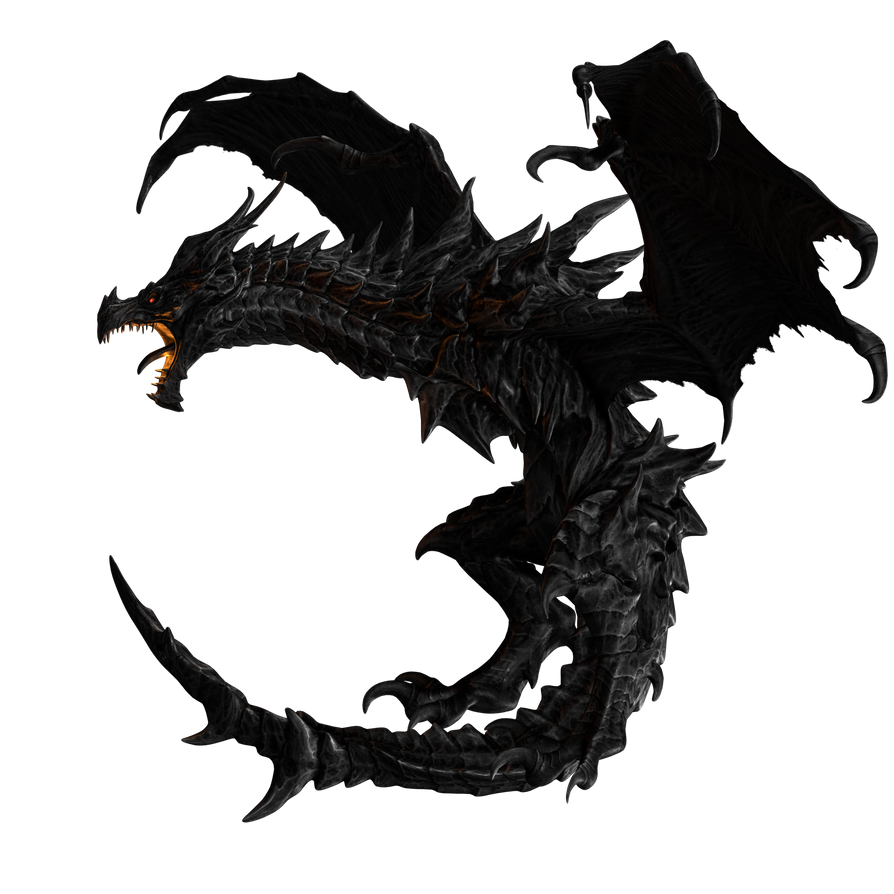
\includegraphics[width=5cm]{other/grim.png}};
    
    % Authors positioned around the outer circle
    \foreach \name/\angle in {Gaurang Pendharkar/0, Varun Ananth/60, I2 Leadership/120,
                              Carter Swartout/180, Arya Sanjay/240, Misha Nivota/300} {
        % Calculate rotation angle for names to be always upright
        \pgfmathparse{\angle<180 ? \angle-90 : \angle+90}
        \ifnum\angle=0
            \pgfmathsetmacro\rot{\angle+90}
        \else
            \pgfmathsetmacro\rot{\pgfmathresult} % Default condition for others
        \fi
        
        % Author names
        \node[rotate=\rot, anchor=mid, font=\bfseries\Large] at (\angle:\Radius) {\name};
        
    }
\end{tikzpicture}\\
\texttt{v1.0} %%% VERSION NUMBER
\newpage

\begingroup
\centering
\section*{The I2 Grimoire}
We are Interactive Intelligence, an organization of interdisciplinary thinkers that seek to probe intelligence through the intersection of AI, neuroscience, and related fields. This book serves as a launchpad for the basic theory that underlies major AI systems and covers five large (intersecting) spheres: Machine Learning, Deep Learning, Computer Vision, Reinforcement Learning, and Language Modeling. While by no means a thorough overview of any one of these fields, this book serves as a starting point that will paint a large picture in your mind about the five aforementioned topics. This book is written in layman's english, and introduces some complex (but core) math while explaining as much intuition behind it as possible. Regardless of your background, there is something interesting you will learn in these pages. Feel free to explore sections that interest you, backtracking if you encounter unfamiliar concepts. \break

This book is a culmination of many months of work by very talented students from the University of Washington. It was entirely created by I2 members, and we hope that you enjoy what we have written in these pages and leave better equipped to navigate this world we share with AI algorithms.

\subsection*{Additional Information}
This book was written to pair with the Interactive Intelligence intro to NeuroAI course, which lives here: \href{https://course.uw-i2.org/}{Interactive Intelligence Intro to NeuroAI Course Website}. There are questions associated with some sections, which serve as optional exercises for you to test your understanding. If you have questions or comments on the information in this book, please contact \href{mailto:varunananth1@gmail.com}{\texttt{varunananth1@gmail.com}} \\
\vspace{2cm}

\includegraphics[scale=0.3]{other/i2-brain.png}
\endgroup

\newpage
\tableofcontents
\newpage

\section*{MACHINE LEARNING}
\addcontentsline{toc}{section}{\protect\numberline{}MACHINE LEARNING}
\section{Introduction to Machine Learning}
    \large Machine Learning (ML) is a powerful subset of artificial intelligence (AI) that empowers computers to learn from data and make predictions or decisions without the need for explicit programming. Rather than following static, rule-based instructions, machine learning models identify patterns, structures, and relationships within data. These models generalize from known data to make predictions about new, unseen data, much like how humans learn from past experiences.
    
    Consider the task of recognizing handwritten digits, like those in postal addresses or bank checks. We can train a machine learning model using a dataset of labeled images, where each image corresponds to a digit from 0 to 9. The model learns to recognize the unique patterns of each digit by analyzing features such as curves, edges, and line intersections. Over time, the model refines its ability to correctly identify digits it has never encountered before, thus demonstrating its ability to generalize from the data it was trained on.
\subsection{Data Splitting: Train and Test Sets}
\large \textbf{Train/Test Split} refers to this method of dividing the dataset, typically using an 80-20 or 70-30 ratio. For example, in an 80-20 split, 80\% of the data is used for training, and the remaining 20\% is held back for testing


The reason we need a test set is to prevent \textbf{overfitting}, a common problem where a model becomes too tailored to the training data, performing well on it but poorly on new data. By evaluating on the test set, we can gauge whether the model has generalized well beyond the data it was trained on.

In practice, the following steps are often taken when working with train/test splits:
\begin{itemize}
    \item \textbf{Step 1: Data Splitting.} Split the data into training and test sets before training the model. This prevents any information from the test set from leaking into the model.
    \item \textbf{Step 2: Model Training.} Use the training set to build the machine learning model by adjusting weights, minimizing errors, or finding patterns.
    \item \textbf{Step 3: Model Evaluation.} Once the model is trained, evaluate it on the test set. Common evaluation metrics include accuracy, precision, recall, and mean squared error, depending on the type of model.
\end{itemize}

In some cases, a third subset called a \textbf{validation set} is also used. The validation set helps tune hyperparameters and prevent overfitting before final testing on the test set.

This train/test split method is fundamental to machine learning as it ensures that models can be assessed on their ability to generalize, avoiding bias toward the data they were trained on.
\subsection{Regression and Classification Tasks}
    \large Machine learning generally tackles two major types of problems: regression and classification.
    
    \textbf{Classification} is the task of categorizing a set of items into predefined classes. For example, classifying an image as either a “cat” or a “dog.” The output is typically a discrete label, such as “yes” or “no,” or in this case, “cat” or “pig.”
    
    On the other hand, \textbf{regression} is about predicting a continuous value. For instance, predicting a person’s weight based on their height is a regression task, where height is the input feature and weight is the predicted continuous value. In multiple regression, multiple features (like height, age, etc.) are used to predict an output, such as house prices or stock market trends.

\section{Linear Regression: Regression}
\subsection{Fundamentals of Linear Regression}
    \large In machine learning, linear regression is one of the most fundamental algorithms. It tries to model the relationship between input features and the target output by fitting a straight line to the data points. The general form of a linear regression model is:
        $$\hat{y} = b + w_1x_1 + w_2x_2 + ... + w_nx_n$$
    Where:
    \begin{itemize}
        \item \( \hat{y} \) is the predicted output,
        \item \( x_1, x_2, ..., x_n \) are the input features,
        \item \( w_1, w_2, ..., w_n \) are the weights (coefficients) assigned to each feature,
        \item \( b \) is the intercept.
    \end{itemize}
    The goal of linear regression is to find the values of \( w \) and \( b \) that minimize the difference between the predicted values and the actual target values in the training data. This is often done by minimizing the Sum of Squared Errors (SSE).
\subsection{Understanding Sum of Squared Errors (SSE)}
    \large The \textbf{Sum of Squared Errors (SSE)} is a commonly used metric in regression analysis to quantify how well a model fits the observed data. It measures the total difference (or error) between the actual values (from the dataset) and the predicted values (generated by the model). Specifically, SSE sums the squared differences between each actual value and its corresponding predicted value. By squaring these differences, the metric ensures that all deviations are counted positively (i.e., large errors in either direction, above or below, contribute significantly to the total error).

    The formula for SSE is:
    \[
        \mathrm{SSE} = \sum_{i=1}^{m} (y_i - \hat{y}_i)^2
    \]
    
    Where:
    \begin{itemize}
        \item \( y_i \) represents the \textbf{actual value} for data point \( i \),
        \item \( \hat{y}_i \) represents the \textbf{predicted value} from the model for the same data point,
        \item \( m \) is the \textbf{number of data points} in the dataset.
    \end{itemize}

    The concept of squaring the errors is essential because it penalizes larger deviations more than smaller ones. In other words, if a prediction is far off from the actual value, its contribution to the SSE will be disproportionately larger, making it easier to identify large errors.

    \begin{figure}[H]
        \centering
        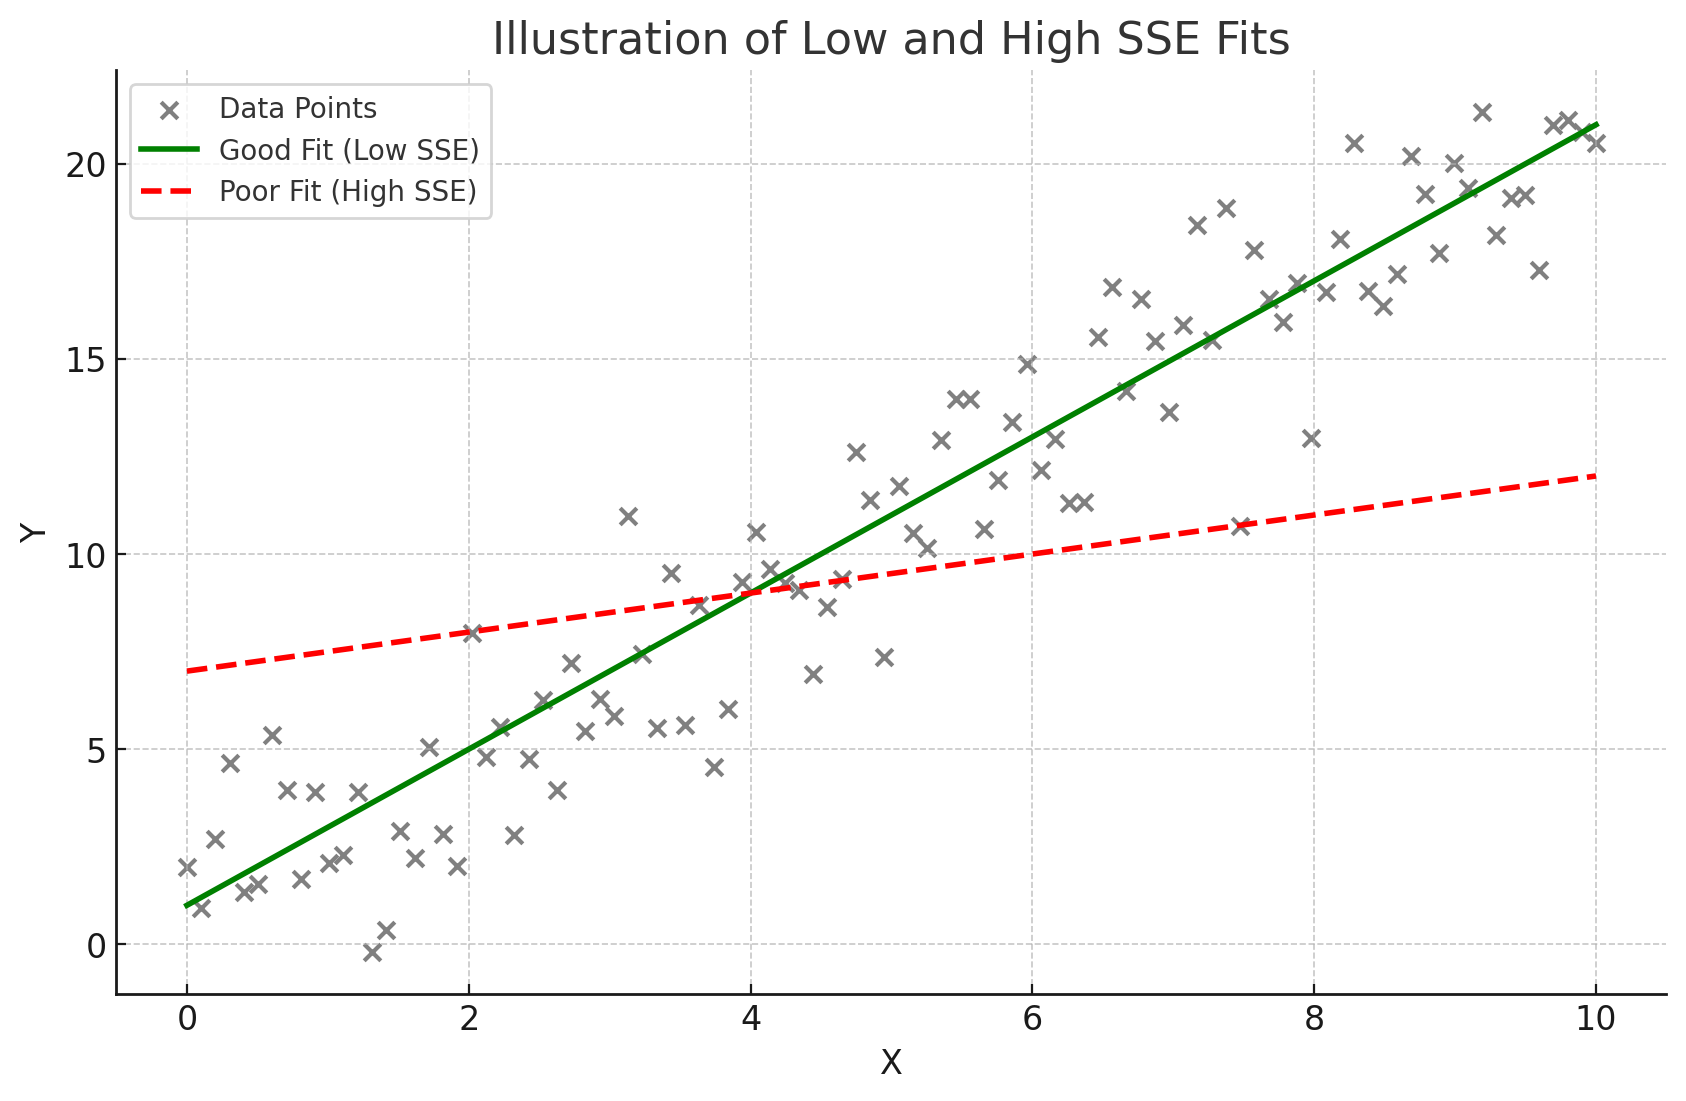
\includegraphics[width=0.45\linewidth]{ml/seefits.png}
        \caption{An illustration of two lines of fit that would produce a low and high SSE respectively. The line that fits the data better has a low SSE}
        \label{fig:seefits}
    \end{figure}

    \textbf{The goal in regression} is to minimize SSE, because a lower SSE value indicates a better fit of the model to the data. A model with a small SSE suggests that its predictions are close to the actual observed values, indicating that the model is accurate and effectively capturing the patterns in the data.
\subsection{Minimizing SSE: Simple Case}
    \large \textbf{Least Squares Regression} is one of the most widely used methods in statistics for finding the best-fitting line through a set of data points. The term “least squares” refers to the fact that the method seeks to minimize the \textbf{sum of squared differences} (i.e., the SSE) between the observed values and the values predicted by the regression line. The result is a line (or, in higher dimensions, a hyperplane) that minimizes the overall prediction error across all data points.

    In simple linear regression, the model is expressed as:
    \begin{center}
        \( \hat{y} = w_0 + w_1x \)
    \end{center}
    Where:
    \begin{itemize}
        \item \( w_0 \) is the \textbf{intercept} of the line, representing the predicted value when the input \( x = 0 \),
        \item \( w_1 \) is the \textbf{slope} or weight, representing the change in the predicted value \( \hat{y} \) for a one-unit change in the input \( x \),
        \item \( x \) is the input (or feature) variable, and
        \item \( \hat{y} \) is the predicted value based on the input.
    \end{itemize}

    In the least squares method, the goal is to find the optimal values for \( w_0 \) and \( w_1 \) that minimize the SSE, ensuring that the line fits the data as closely as possible. The same concept can be extended to multiple regression, where we aim to minimize the SSE by adjusting multiple weights \( w_1, w_2, ..., w_n \).

    Mathematically, this optimization process requires taking the partial derivatives of SSE with respect to the weights (including the intercept) and setting them to zero. This gives us the \textbf{normal equations}:
    \begin{center}
        \( w_0 = \frac{\sum y - w_1\sum x}{n} \)
    \end{center}
    \begin{center}
        \( w_1 = \frac{\sum(x_i - \bar{x})(y_i - \bar{y})}{\sum(x_i - \bar{x})^2} \)
    \end{center}

    These equations provide the values of the intercept (\( w_0 \)) and the slope (\( w_1 \)) that minimize SSE. Once these values are calculated, the resulting regression line represents the best-fitting line for the data according to the least squares criterion.
\subsection{Minimizing SSE: General Case}
    \large What if you had a model with many more input features, like the one we showed at the beginning of the article?

    $$\hat{y} = b + w_1x_1 + w_2x_2 + ... + w_nx_n$$

    It becomes much easier to represent the solution for the weights in matrix form. However, we need to translate what we have here into matrix form first.
    
    We first define $\textbf{w}$ as a vector consisting of all the weights in our model:

    $$\textbf{w} = \begin{bmatrix}
            w_1\\
            w_2\\
            \vdots\\
            w_n\\
            \end{bmatrix}$$

    Our goal is to find $\hat{\textbf{w}}$, the weights for our model that minimize the SSE. Similarly, we define $\textbf{x}_i$ as a vector consisting of all the features \textit{of a single datapoint}:
    $$\textbf{x}_i = \begin{bmatrix}
            x_1\\
            x_2\\
            \vdots\\
            x_n\\
            \end{bmatrix}$$
    You can think of each $\textbf{x}_i$ as a point in n-dimensional space. We denote this mathematically as $\textbf{x}_i \in \mathbb{R}^n$. Using this, we can define $X$ as a matrix holding all of our $m$ datapoints:
    $$X = \begin{bmatrix}
            \textbf{x}_1^{\top}\\
            \textbf{x}_2^{\top}\\
            \vdots\\
            \textbf{x}_m^{\top}\\
            \end{bmatrix}$$
    We say that $X \in \mathbb{R}^{m \times n}$. Finally, we define $\textbf{y}$ as a vector holding all of our true labels $y$ from our training set.
    $$\textbf{y} = \begin{bmatrix}
            y_1\\
            y_2\\
            \vdots\\
            y_m\\
            \end{bmatrix}$$
    The amount of $y$ values is the same as the amount of $x$ points ($m$). Using these elements, we can actually very easily construct a closed-form solution to $\hat{\textbf{w}}$!

    $$\hat{\textbf{w}} = (X^{\top}X)^{-1}X^{\top}\textbf{y}$$

    How to derive this is a tad beyond the scope of this article, especially if you are unfamiliar with matrix calculus. However, the proof is provided below for thoroughness. For a quick refresher on matrix algebra, see \href{https://www.youtube.com/playlist?list=PLZHQObOWTQDNU6R1_67000Dx_ZCJB-3pi}{Essence of Linear Algebra Series by 3Blue1Brown}. For a quick refresher on matrix calculus, see \href{https://www.youtube.com/watch?v=tIkzL4jlt8g}{Matrix Calculus for Machine Learning by StatQuest}.
    \begin{align*}
        \hat{\textbf{w}} &= \argmin_w \sum_{i=1}^n (y_i - \hat{y}_i)^2 && \text{Find $\textbf{w}$ that minimizes the SSE. This is $\hat{\textbf{w}}$.}\\
        &= \argmin_w \sum_{i=1}^n (y_i - (\textbf{x}_i^{\top}\textbf{w} + b))^2 && \text{Plug in $\hat{y}_i = \textbf{x}_i^{\top}\textbf{w} + b$.}\\
        &= \argmin_w \sum_{i=1}^n (y_i - (\textbf{x}_i^{\top}\textbf{w}))^2 && \text{\parbox{0.5\textwidth}{Disregard $b$, since an intercept can be represented by appending a 1 to $\textbf{x}$.}}\\
        0 &= \frac{\partial}{\partial w} \sum_{i=1}^n (y_i - (\textbf{x}_i^{\top}\hat{\textbf{w}}))^2 && \text{\parbox{0.5\textwidth}{Find $\hat{\textbf{w}}$ by taking the partial derivative of the argmin term and setting it equal to 0.}}\\
        &= \sum_{i=1}^n \frac{\partial}{\partial w} (y_i - (\textbf{x}_i^{\top}\hat{\textbf{w}}))^2 && \text{Property of derivatives.}\\
        &= \sum_{i=1}^n 2(y_i - \textbf{x}_i^{\top}\hat{\textbf{w}})(-\textbf{x}_i) && \text{Derive.}\\
        &= \sum_{i=1}^n (y_i - \textbf{x}_i^{\top}\hat{\textbf{w}})(
        \textbf{x}_i) && \text{Divide by -2}\\
        &= \sum_{i=1}^n (
        \textbf{x}_i)(y_i - \textbf{x}_i^{\top}\hat{\textbf{w}}) && \text{The term $y_i - \textbf{x}_i^{\top}\hat{\textbf{w}}$ is a scalar. $c\textbf{x} = \textbf{x}c$}\\
        &= \sum_{i=1}^n (\textbf{x}_iy_i - \textbf{x}_i\textbf{x}_i^{\top}\hat{\textbf{w}}) && \text{Distribute}\\
        &= \sum_{i=1}^n \textbf{x}_iy_i - \sum_{i=1}^n \textbf{x}_i\textbf{x}_i^{\top}\hat{\textbf{w}} && \text{Distribute}\\
        (\sum_{i=1}^n \textbf{x}_i\textbf{x}_i^{\top})\hat{\textbf{w}} &= \sum_{i=1}^n \textbf{x}_iy_i && \text{Move second term to LHS.}\\
        (X^{\top}X)\hat{\textbf{w}} &= X^{\top}\textbf{y} && \text{\parbox{0.5\textwidth}{Convert from vector summation form to matrix form}}\\\\
        (X^{\top}X)^{-1}(X^{\top}X)\hat{\textbf{w}} &= (X^{\top}X)^{-1}X^{\top}\textbf{y} && \text{Left multiply by $(X^{\top}X)^{-1}$}\\
        \hat{\textbf{w}} &= (X^{\top}X)^{-1}X^{\top}\textbf{y} && \text{Cancel}\\
    \end{align*}

    This is pretty amazing. If you were to create just $X$ and $\textbf{y}$ for any regression dataset, you can find $\hat{\textbf{w}}$. It doesn't matter how many features you have, this will work. We also know \textit{for a fact} that these weights in $\hat{\textbf{w}}$ are the weights that will minimize the SSE the most due to a property called \textbf{convexity}. We will come back to what this is later. In addition to linear regression, we have two other very common types of regression called Ridge and LASSO.

\subsection{Ridge and LASSO Regressions}
    \large We must first quickly introduce a concept called \textbf{regularization}. Quite often, you will find that the weights estimated by $\hat{\textbf{w}}$ do minimize the SSE for training data, but can perform poorly on real-world data post model deployment. This is because the weights found are \textit{too well tuned} to the training data, and cannot generalize with the same performance to unseen data. What can also happen is that some weights will become very large, since the feature they are associated with is important for predicting $y_i$. Let's say we are training a regression model to predict house prices based on house features. One feature could indicate if a house is a lakefront property. Since our training data is primarily from Florida, the indication of a lakefront property means that the property has a very high value. So, the model basically \textit{just} uses this one feature to predict housing price. All other features have their associated weights very low, meaning they barely influence the model's output. The model works just fine for houses in Florida. However, when we go to predict the prices of houses in Wyoming, we see that none of them are lakefront properties and therefore this feature that the model placed so much importance on has become useless. The model ``put all its eggs in one basket'' and now has poor performance on real data despite performing wonderfully on the training set! We will explore this concept further when talking about the \textbf{bias-variance tradeoff}, but for now just understand that the weights you find with ordinary linear regression tend to not generalize well.

    \begin{figure}[H]
        \centering
        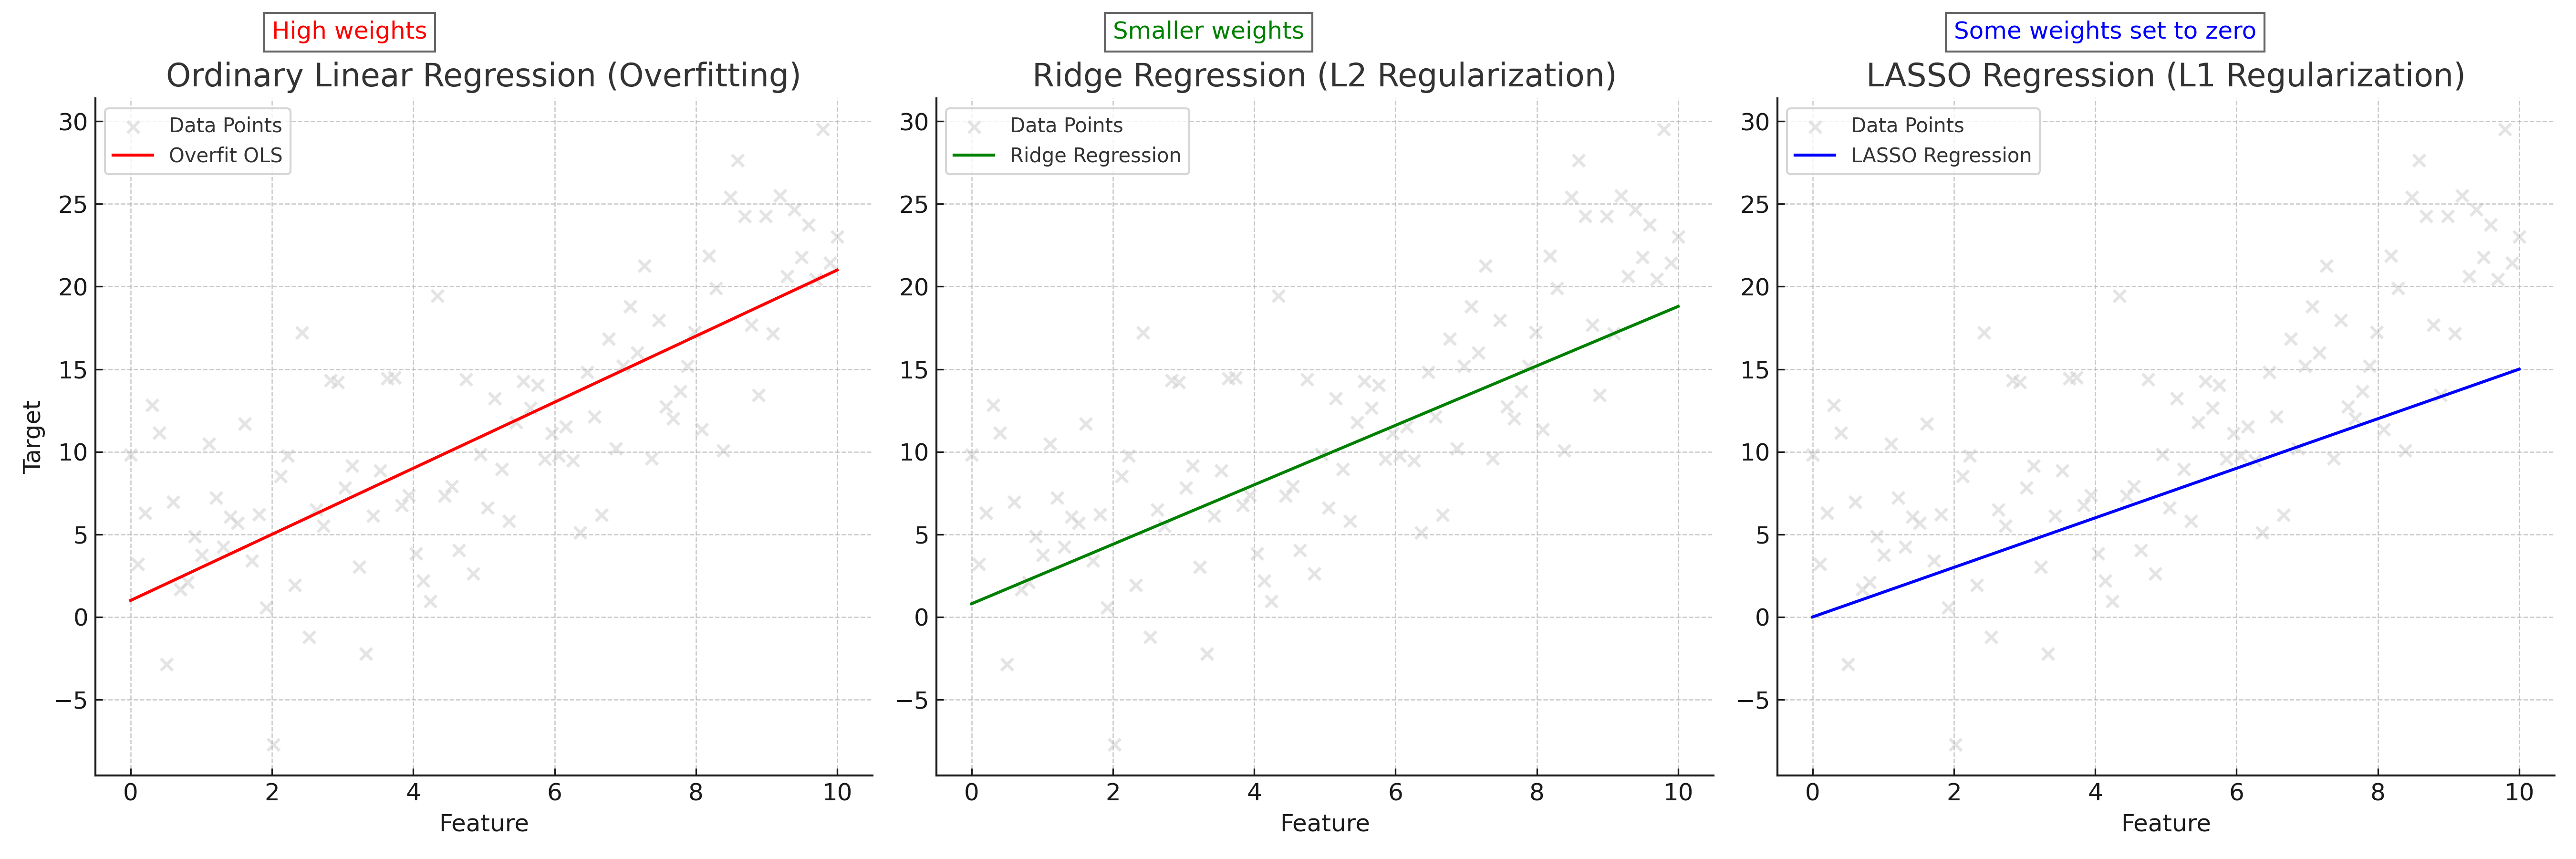
\includegraphics[width=0.85\linewidth]{ml/regression_comparison.png}
        \label{fig:regression_comparison}
    \end{figure}
    
    What can we do in this case? Well, we can penalize weights becoming too high by modifying our SSE optimization objective to include a term that increases as the weights do. This will encourage the model to find a solution for $\hat{\textbf{w}}$ while keeping the weights more balanced. What this term is determines which linear regression variant we get. If we use the L2-norm, we get \textbf{Ridge regression}. If we use the L1-norm, we get \textbf{LASSO} regression. If we use both, we get \textbf{ElasticNet}. This last model is beyond the scope of this article, but we will explore how the first two behave.

    But first, what are the L2 and L1 norms? These norms are mathematical functions that map from vector space to scalar space ($\mathbb{R}^n \rightarrow \mathbb{R}$). They are defined as such:

    \begin{align*}
      \|\textbf{x}\|_2 &= \sqrt{\sum_{i=1}^n x_i^2} \\
      \|\textbf{x}\|_1 &= \sum_{i=1}^n \vert x_i \vert
    \end{align*}

    So the L2 norm is the square root of the sum of squared elements from the vector, and the L1 norm is the sum of the absolute value of elements from the vector. These are our regularizers. If we calculate these norms on $\hat{\textbf{w}}$, you can see that the result gets larger if the elements of $\hat{\textbf{w}}$ are large/unbalanced (something we don't want). We want to find a solution that attempts to minimize $||\hat{\textbf{w}}||_2$ or $||\hat{\textbf{w}}||_1$ along with the original SSE objective. We therefore write our two new optimization objectives down:

    \begin{align*}
      \text{Ridge SSE} &= \sum_{i=1}^{m} (y_i - \hat{y}_i)^2 + \lambda\|\hat{\textbf{w}}\|_2 \\
      \text{LASSO SSE} &= \sum_{i=1}^{m} (y_i - \hat{y}_i)^2 + \lambda\|\hat{\textbf{w}}\|_1
    \end{align*}

    The $\lambda$ term allows us to control how much regularization we want. A small number makes the mode kind of ``care'' about keeping its weights down. A large value forces the model to keep its weights down at the expense of weights that actually fit the data. Finding the right value for $\lambda$ is a balancing act.

    As for how to actually find $\hat{\textbf{w}}$ for these new optimization objectives, that is a little tricky. Ridge regression has a closed-form solution that can be derived similar to ordinary linear regression. It also looks quite similar:

    $$\hat{\textbf{w}} = (X^{\top}X + \lambda I)^{-1}X^{\top}\textbf{y}$$

    $I$ is the identity matrix, a $\mathbb{R}^{n \times n}$ matrix in this case with ones down the diagonal and zeroes everywhere else. How this comes about is hidden in the algebra and calculus of the derivation. That derivation is much beyond the scope of this article, but not impossible to understand if you grasp the ordinary linear regression closed form solution derivation. For LASSO, you have to use more complex techniques like variations of \textbf{gradient descent}. We will cover this topic in later units.

    What is the difference between these two linear regression variants? If you use Ridge regression, your final $\hat{\textbf{w}}$ value will have weights that are low and spread out across all features. If you use LASSO regression, you will get a ``sparse'' $\hat{\textbf{w}}$, meaning that unimportant features will have their weights set to 0 and the important ones will have nonzero values. This is due to how the norms manifest on the ``loss landscape''. As shown in Figure \ref{fig:l1_l2}, the solution (minima) to the Ridge SSE or LASSO SSE must sit on the intersection of the a contour (oval) and the shape created by the norm. For L1, this norm has peaks at the axes, causing solutions to have zero values for $w_1$ but nonzero values for $w_2$. The L2 norm is less harsh, with a lower but nonzero value for $w_1$. Cranking up $\lambda$ will exaggerate these effects, with incredibly high values for $\lambda$ in LASSO regression resulting in only one or two features having non-zero weights.

    \begin{figure}[H]
        \centering
        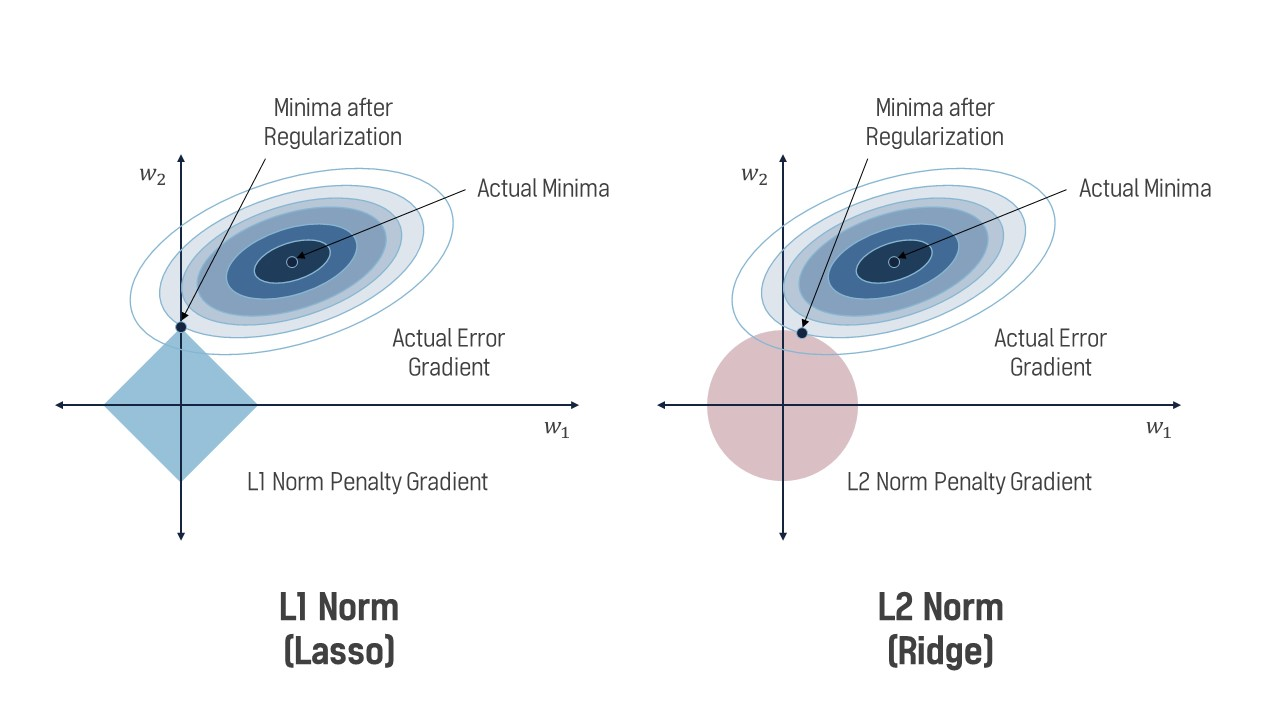
\includegraphics[width=0.9\linewidth]{ml/l1_l2.jpg}
        \caption{Showing how the L1 and L2 norms influence $\hat{\textbf{w}}$ through the nature of their manifestations on the loss landscape as a hyperdiamond and hypersphere respectively}
        \label{fig:l1_l2}
    \end{figure}

    Both of these regression variants have use cases where they shine, so no one is ``better'' than the other. Ridge regression should be used when you want to ensure all features influence the final output, and you should use LASSO when you want to perform intelligent ``feature pruning'' and only use relevant features for the final output (perhaps due to computational constraints).

\begin{questionbox}
\textbf{Synthesis Questions:}
\begin{enumerate}
    \item What is SSE? Why do we want to minimize it?
    \item What do the following symbols represent, and what are their shapes? (Assume $n$ is the dimensionality of the data and $m$ is the number of datapoints):
    \begin{itemize}
        \item $\textbf{w}$
        \item $\hat{\textbf{w}}$
        \item $X$
        \item $\textbf{y}$
    \end{itemize}
    \item Rewrite the euclidean distance formula $d(x,y) = \sqrt{\sum_{i=1}^n (x_i-y_i)^2}$ using the L2-norm $||\textbf{x}||$ given two vectors $\textbf{x}$ and $\textbf{y}$. Do you notice any relationship between the L2-norm and euclidean distance?
    \item In your own words, what are the differences between Ordinary, Ridge, and LASSO regressions?
    \item \textbf{Bonus:} Solve for $\hat{\textbf{w}}$ in the Ridge regression setting. Here is the equation:
      \[\argmin_{\hat{\mathbf{w}}} \sum_{i=1}^n (y_i - \hat{y}_i)^2 + \lambda||\hat{\textbf{w}}||_2^2.\]
      Your answer should be the closed form solution for Ridge regression and the proof should be similar to the one given for ordinary linear regression.
\end{enumerate}
\end{questionbox}

\section{Logistic Regression: Classification}
\subsection{Fundamentals of Logistic Regression}
    \large Logistic regression, despite its name, is a classification algorithm used to predict a binary outcome—often represented as a “yes/no” or “1/0.” Unlike linear regression, which predicts continuous values, logistic regression is designed to output the probability that a given input belongs to a certain class. For instance, it can help us predict if an email is spam or not based on various features.

    The fundamental idea behind logistic regression is to use a \textbf{sigmoid function} to transform the output of a linear equation (a combination of input variables) into a probability between 0 and 1. The probability tells us how likely the input belongs to one of two possible classes, usually denoted as 1 (positive class) or 0 (negative class). The sigmoid function is defined as:

    \begin{center}
        \( P(y=1 \mid x) = \frac{1}{1 + e^{-(b + w^{\top}x)}} \)
    \end{center}
    
    Where:
    \begin{itemize}
        \item \( w \) is the \textbf{weight vector}, which defines the importance of each feature in the input.
        \item \( b \) is the \textbf{bias term}, which adjusts the overall output of the function.
        \item \( e \) is Euler’s number, and the exponent ensures that the output is squeezed between 0 and 1.
    \end{itemize}

\subsection{The Sigmoid Function and Its Role}
    \begin{figure}[H]
        \centering
        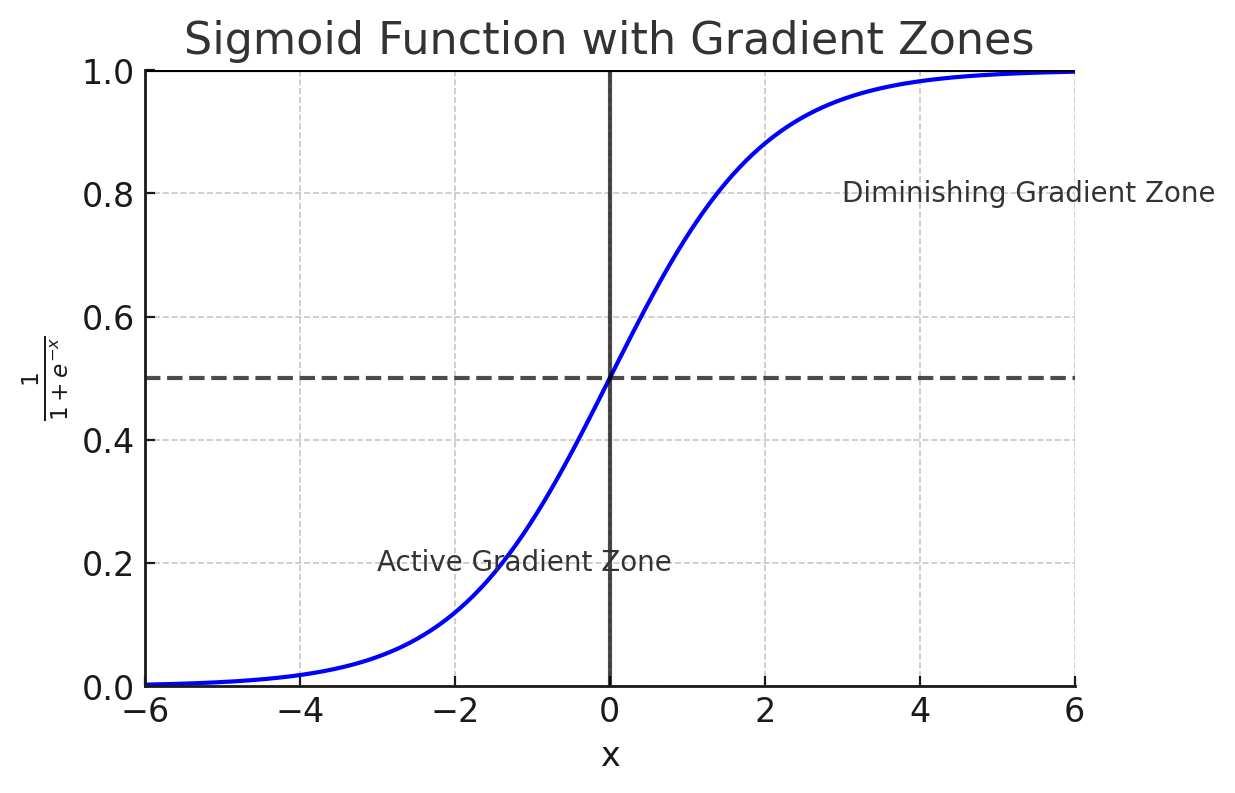
\includegraphics[width=0.45\linewidth]{ml/sigmoid_function.png}
        \caption{A graph showing the sigmoid function.}
        \label{fig:sigmoid_function}
    \end{figure}
    
    \large The sigmoid function plays a crucial role in logistic regression because it takes any input from the linear equation and converts it into a value between 0 and 1. This value can be interpreted as a probability, helping us decide which class the input most likely belongs to. Here's how it works:
    
    \begin{itemize}
        \item If the result of the linear equation (\( b + w^{\top}x \)) is a large positive number, the sigmoid function outputs a value close to 1, indicating that the input most likely belongs to class 1.
        \item If the result is a large negative number, the sigmoid function outputs a value close to 0, indicating class 0.
        \item If the result is near 0, the sigmoid outputs a value close to 0.5, meaning the input is equally likely to belong to either class.
    \end{itemize}
    
    This probability can then be used to classify the input: if the probability is greater than 0.5, we predict class 1, and if it is less than 0.5, we predict class 0.

\subsection{Training with the Log-Likelihood Loss}
    \large To make logistic regression work effectively, we need to find the best values for the weights \( w \) and bias \( b \). This is done by minimizing the \textbf{log-likelihood loss function}. This function measures how well the model’s predicted probabilities match the actual class labels. By adjusting the weights and bias to minimize this loss, we ensure that the model produces the most accurate predictions.

    During training, the model learns to minimize this loss by using optimization techniques like gradient descent. This ensures that the weights are fine-tuned to give the highest probability for the correct class as often as possible.

\subsection{Extensions to Multiclass Classification}
    \large While logistic regression is primarily used for binary classification, it can be extended to handle multiple classes through methods such as \textbf{one-vs-rest (OvR)}. In this approach, we train multiple logistic regression models, each one responsible for distinguishing whether an input belongs to one particular class or any of the others. The model with the highest probability ultimately decides the final class label.

\subsection{Why It's Called “Regression”}
    \large The term ``logistic regression'' comes from its similarity to \textbf{linear regression}. Both methods start by calculating a linear combination of the input features. However, while linear regression outputs continuous values, logistic regression uses the sigmoid function to turn these values into probabilities, which are used for classification tasks. This difference is crucial to understanding why logistic regression is a classification algorithm despite having ``regression'' in its name.

\begin{questionbox}
\textbf{Synthesis Questions:}
\begin{enumerate}
    \item How does the sigmoid function play a role in making Logistic Regression a classification algorithm?
    \item For the algorithm to say that the input is equally likely to be from either class, what must have $b + w^{\top}x$ have been?
\end{enumerate}
\end{questionbox}

\section{K-Means Clustering: Unsupervised Learning}
\subsection{Introduction to Unsupervised Learning}
    \large In contrast to supervised learning, which learns from labeled data, \textbf{unsupervised learning} operates on \textbf{unlabeled data} and aims to find hidden patterns or structures within it. One powerful method used in unsupervised learning is \textbf{k-means clustering}. This algorithm attempts to group data points into \( k \) clusters, where each cluster contains points that are similar to each other. Unlike supervised methods where there is a clear ``right answer'', the objective here is to let the algorithm uncover these clusters on its own.

\subsection{How K-Means Clustering Works}
    \large At its core, k-means clustering is about finding the best way to group data points. This process involves iteratively assigning data points to clusters and then recalculating the center of each cluster, known as the \textbf{centroid}. The idea is to minimize the distance between data points and their corresponding centroids, so points within a cluster are more similar to each other than to points in other clusters.

    The process of k-means clustering can be broken down into the following steps:
    \begin{itemize}
        \item \textbf{Step 1: Initialization.} The algorithm begins by randomly selecting \( k \) initial cluster centroids from the dataset. These centroids act as the starting points for the clusters.
        
        \item \textbf{Step 2: Assignment.} Each data point is assigned to the nearest centroid based on a distance metric, typically Euclidean distance. This forms \( k \) clusters of data points, with each point belonging to the cluster whose centroid is closest.
        
        \item \textbf{Step 3: Update.} Once the points are assigned to clusters, the centroids of the clusters are recalculated. The new centroid is the mean of all the data points in the cluster.
        
        \item \textbf{Step 4: Repeat.} Steps 2 and 3 are repeated until the centroids no longer move significantly, or the cluster assignments do not change. This indicates that the algorithm has converged.
    \end{itemize}

    The goal of this process is to minimize the sum of squared distances between each data point and its cluster’s centroid. This ensures that points in the same cluster are as close to each other as possible.

\subsection{Minimizing Within-Cluster Distance}
    \large In k-means clustering, the objective is to reduce the \textbf{within-cluster variance}, or in simpler terms, the total distance between the data points and the centroid of their assigned cluster. The function to minimize is called the \textbf{sum of squared errors} (SSE), which measures how far the data points are from their respective cluster centroids:
    \[
    \mathrm{SSE} = \sum_{j=1}^{k} \sum_{x_i \in C_j} \|x_i - \mu_j\|^2
    \]
    Where:
    \begin{itemize}
        \item \( x_i \) represents a data point,
        \item \( \mu_j \) is the centroid of cluster \( j \),
        \item \( C_j \) represents the set of points assigned to cluster \( j \),
        \item \( \|\cdot\|^2 \) is the squared Euclidean distance.
    \end{itemize}
    
    By minimizing the SSE, k-means clustering ensures that data points within the same cluster are tightly packed around their centroid, making the clustering meaningful.

\subsection{Choosing the Number of Clusters}
    \large A critical decision in k-means clustering is determining the value of \( k \), or how many clusters the data should be divided into. Often, this is not known in advance, so techniques such as the \textbf{elbow method} are used. In the elbow method, the SSE is calculated for various values of \( k \), and the results are plotted. The ``elbow'' point on the plot represents the optimal number of clusters—beyond this point, increasing \( k \) provides diminishing returns in terms of reducing SSE.

    \begin{figure}[H]
        \centering
        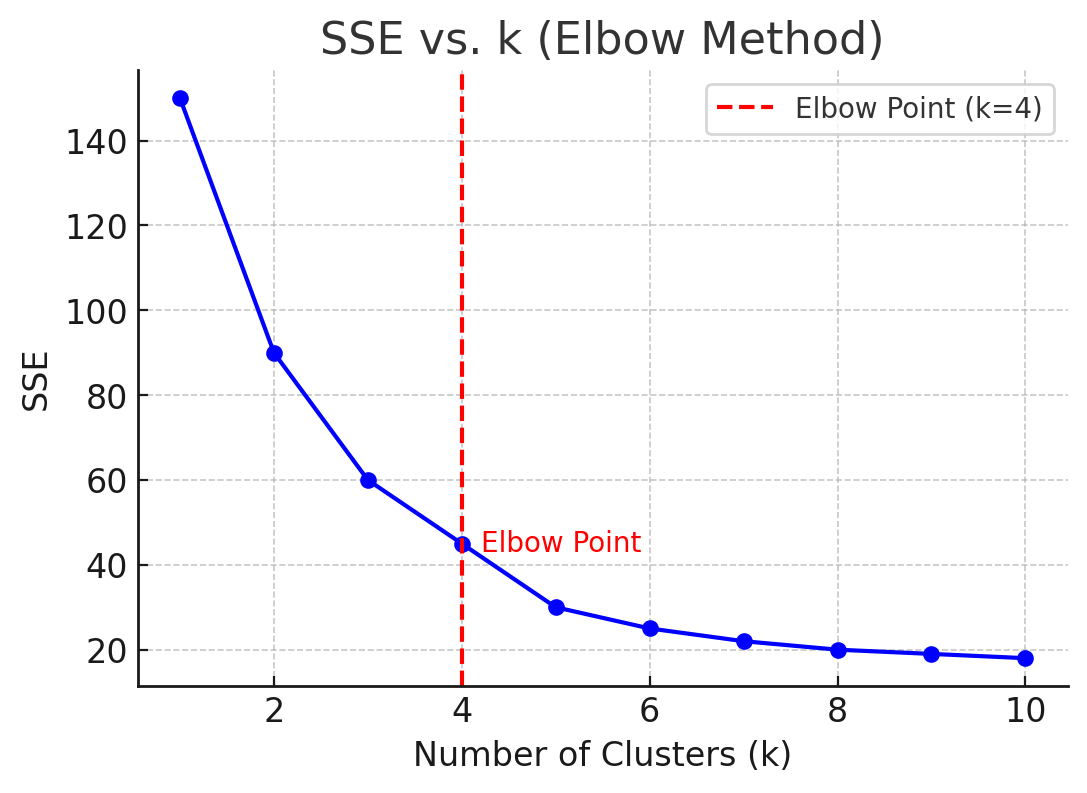
\includegraphics[width=0.45\linewidth]{ml/SSEkElbowmethod.png}
        \caption{An example of a graph showing SSE vs. $k$, and the elbow that can be used to pick the optimal $k$.}
        \label{fig:SSEkElbowmethod}
    \end{figure}

    Another method to determine \( k \) is by using the \textbf{silhouette score}, which evaluates how similar a data point is to its assigned cluster compared to other clusters. Higher silhouette scores indicate better-defined clusters.

\subsection{Limitations of K-Means Clustering}
    \large While k-means is an effective clustering algorithm, it comes with several limitations:
    
    \begin{itemize}
        \item \textbf{Sensitivity to Initialization.} The algorithm is highly sensitive to the initial placement of the centroids. Poor initial choices can result in suboptimal clusters or even cause the algorithm to converge to a local minimum. To address this, a more refined initialization method, \textbf{K-Means++}, is often used to improve the initial centroids.
        
        \item \textbf{Fixed Number of Clusters.} K-means requires that \( k \) be defined ahead of time, which might not always be clear from the dataset. This adds complexity to its usage.
        
        \item \textbf{Sensitivity to Outliers.} K-means clustering can be significantly impacted by outliers. Since the algorithm seeks to minimize distances, outliers (data points far from the rest of the data) can disproportionately affect the cluster centroids.
    \end{itemize}
    
    Despite these limitations, k-means remains a widely used and powerful clustering technique for discovering patterns in data, particularly when the data is well-structured and the number of clusters is approximately known.

\begin{questionbox}
\textbf{Synthesis Questions:}
\begin{enumerate}
    \item Define ``Unsupervised Learning'' and how it is different than ``Supervised Learning''.
    \item What is a centroid? How is it calculated?
    \item If the calculated centroids do not move very much after a few iterations, what does this indicate?
    \item If you have $n$ points to cluster, what value of $k$ will give the lowest SSE no matter how the points are formed? (\textbf{Hint:} It's kind of a cheap, degenerate case!)
    \item Why do you think k-means clustering is sensitive to centroid initialization?
\end{enumerate}
\end{questionbox}

\section{K-Means vs. K-Medians Clustering}
\subsection{Introduction to K-Medians Clustering}
    \large While \textbf{k-means} is a widely used method for clustering, an alternative approach is \textbf{k-medians clustering}, which offers a different way of calculating cluster centers. Instead of using the mean of the data points to define the cluster center as k-means does, k-medians calculates the center as the \textbf{median} of the data points in the cluster. This key difference makes k-medians more robust, particularly in the presence of \textbf{outliers}, as the median is less sensitive to extreme values.
    
    In k-medians, the objective is to minimize the sum of \textbf{absolute differences} between data points and the cluster center, rather than the sum of squared distances. This approach results in cluster centroids that are less influenced by anomalous data points, providing a more stable representation of the typical cluster member in datasets with noisy or skewed distributions.

\subsection{K-Medians Use Cases}
    \large \textbf{K-medians} clustering is especially useful in situations where the data contains significant \textbf{outliers} or when using non-Euclidean distance metrics. Unlike k-means, which can be overly influenced by extreme values due to its reliance on the mean, k-medians offers a more \textbf{robust} solution by focusing on the median. For example, if a dataset contains several unusually large or small values that could distort the cluster centroid under k-means, k-medians will provide a more accurate and representative clustering result.

    K-medians is typically used when minimizing the \textbf{sum of absolute differences} between points is more meaningful than minimizing squared differences, such as in scenarios where data points vary widely in scale or when outliers are frequent. While k-medians may be less common than k-means in practice, it proves highly effective when the assumptions behind k-means (such as normal distribution of data or minimal outliers) do not hold.

\subsection{Key Differences Between K-Means and K-Medians}
    \large The fundamental difference between \textbf{k-means} and \textbf{k-medians} lies in how they compute the cluster centroids and the distance metrics they use. K-means calculates the centroid as the \textbf{mean}, minimizing the sum of squared Euclidean distances. In contrast, k-medians uses the \textbf{median}, minimizing the sum of absolute distances (often referred to as Manhattan distance).

    Here are key distinctions between the two methods:
    
    \begin{itemize}
        \item \textbf{K-Means:} More sensitive to outliers because the mean is influenced by extreme values. It is best suited for datasets where the distance between points is naturally measured using Euclidean distances, and when the data does not contain many outliers.
        
        \item \textbf{K-Medians:} More robust to outliers, as the median remains stable even in the presence of extreme values. It is better suited for datasets with skewed distributions or where minimizing absolute differences is a priority.
    \end{itemize}

    \begin{figure}[H]
        \centering
        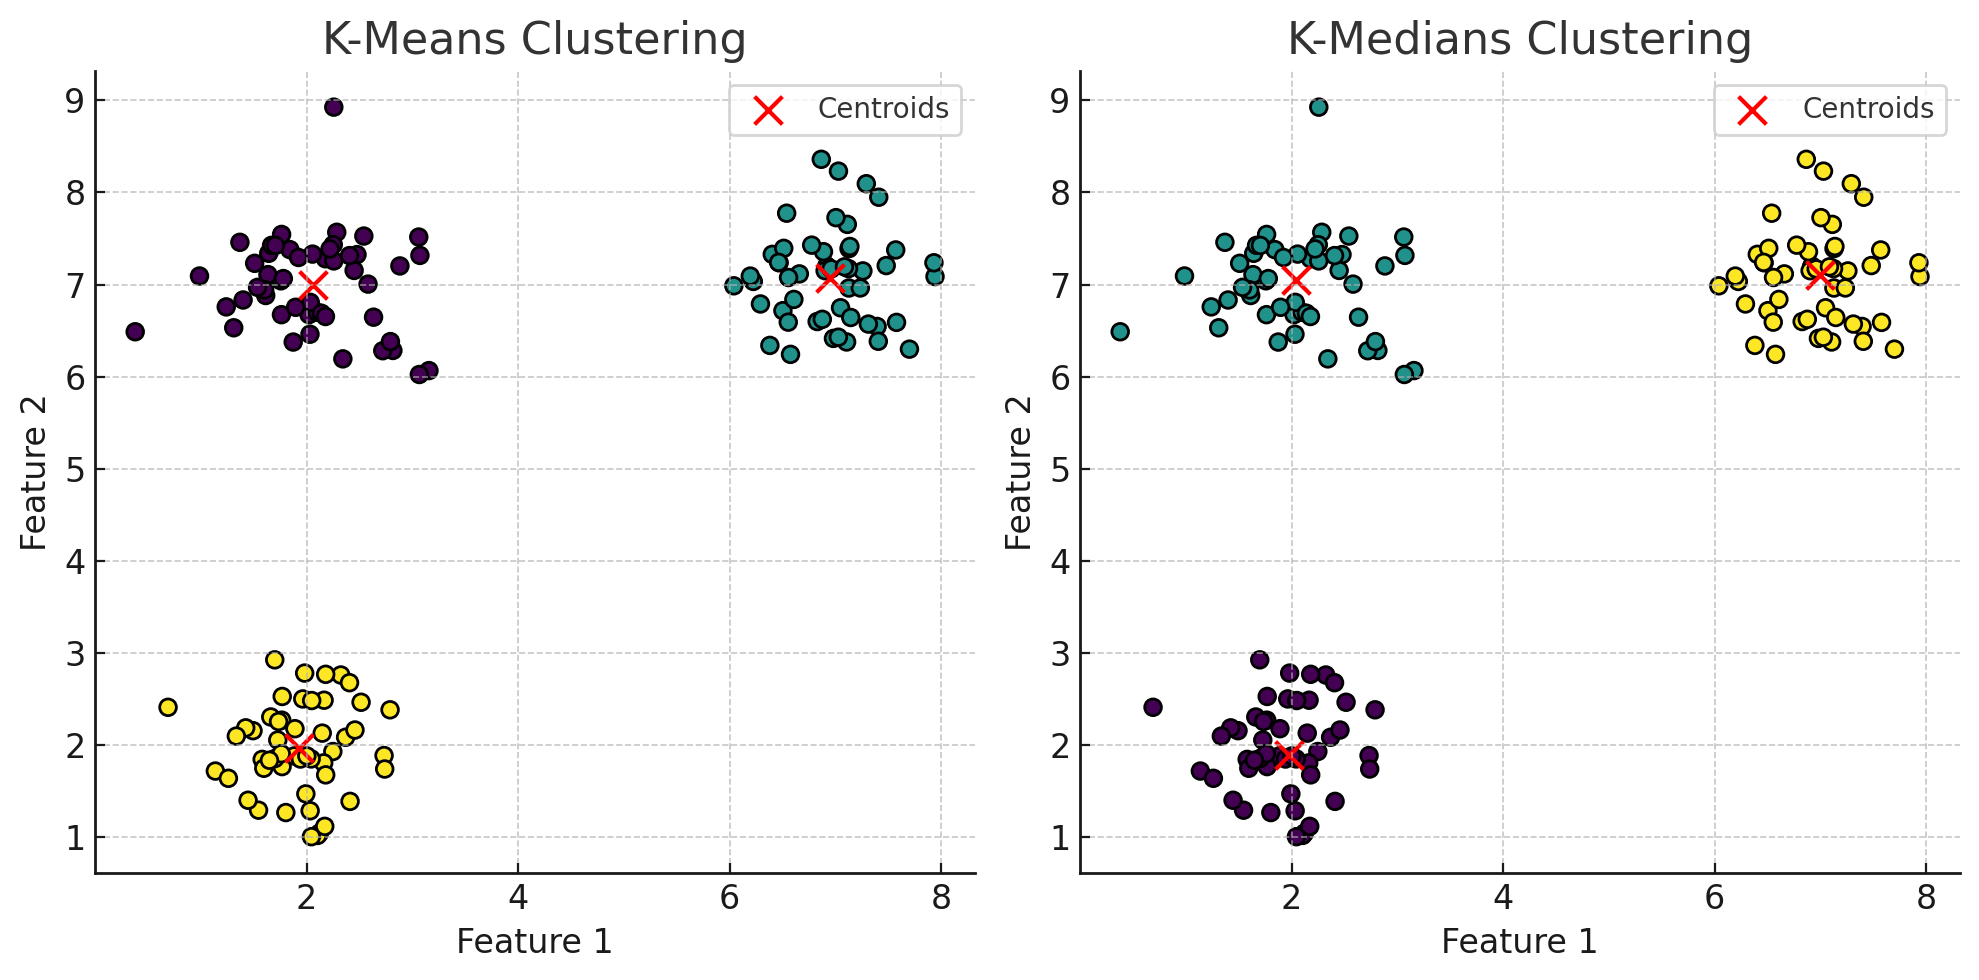
\includegraphics[width=0.45\linewidth]{ml/K-clustering.png}
        \caption{ An image comparing and contrasted the clusters created from k-means and k-medians methods.}
        \label{fig:K-clustering}
    \end{figure}
    
    The choice between the two methods depends heavily on the nature of the dataset. K-means is computationally more efficient but may produce distorted clusters in datasets with many outliers, whereas k-medians offers a more resilient solution for datasets with irregularities or noise.

\begin{questionbox}
\textbf{Synthesis Questions:}
\begin{enumerate}
    \item Give a concrete, real-world example of a situation where \textit{k-means} clustering is a better choice than \textit{k-medians} clustering
    \item Give a concrete, real-world example of a situation where \textit{k-medians} clustering is a better choice than \textit{k-means} clustering
    \item Give a concrete, real-world example of a situation where \textit{neither} of these algorithms will work well
\end{enumerate}
\end{questionbox}

\section{Other ML Concepts}
\subsection{Bias-Variance Tradeoff}
    \large This is a concept that doesn't really fit anywhere else, but is incredibly important to talk about. The bias-variance tradeoff heavily rates to over and underfitting. \textbf{Overfitting} is when you have a model that fits the data it is trained on \textit{too} well. This could come about by, for example, trying to fit a very high-order polynomial curve to data that is linearly correlated. Instead of creating a line of best fit through the data, a sufficiently complex polynomial could just weave through every point in the graph. This would result in 0 SSE, but terrible performance on real-world data after the model is deployed. This is because real data is noisy, and a sufficiently complex model will fit to that noise because doing that technically minimizes SSE. \textbf{Underfitting} is the exact opposite problem. Say you had some synthetic data that took the shape of a parabola, but tried to fit a straight line to it. No matter how many training examples you provide, your model is not complex enough (you can also say it is not \textit{expressive} enough) to fit to the curve well.

    An example of a very basic, not-so-expressive linear model:

    $$y = w_1x_1 + b$$

    An example of a very expressive 5th-degree polynomial model:

    $$y = w_1x_1 + w_2x_1^2 + w_3x_1^3 + w_4x_1^4 + w_5x_1^5 + b$$

    A rarer, but still useful sinusoidal model:

    $$y = w_1\textrm{sin}(w_2x_1 - w_3) + b$$

    When people talk about the bias-variance tradeoff, they are essentially referring to over and under fitting, but are being a little more specific. \textbf{Bias} refers to how close the model line is to the ``true'' underlying curve. You can generate synthetic data for a line by generating points from some $y = mx +b$, but then adding a noise term $\epsilon \sim N(0, 1)$ to each point. If your underlying model fits to the generating $y = mx+b$ but ignores the noise introduced with $\epsilon$, then it has \textit{low bias}. \textbf{Variance} is a bit more complicated, but it essentially concerns the robustness of the model. If you were to add or remove a few points from a dataset, then a model with the appropriate level of expressivity should not change its learned coefficients by much. For example, if you had data correlating age with height, you shouldn't expect removing one or two points to affect the underlying correlation. A overly expressive model would, however, completely refit to swerve through all the points in a new way which drastically changes the coefficients. Variance measures how inconsistent the model is across different training subsets. When fitting ML models, you want a model that minimizes both bias \textit{and} variance. To do this, you must pick a ML model that has enough expressive power to capture underlying trends, but is not so expressive that it suffers from high variance errors. 

    \begin{figure}[H]
        \centering
        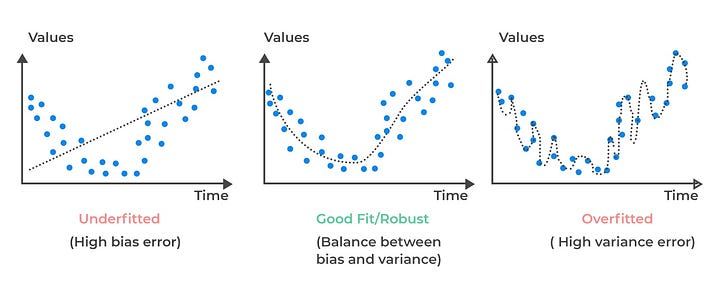
\includegraphics[width=0.8\linewidth]{ml/biasvariance.jpg}
        \caption{An illustration visualizing different balances between bias and variance for model fitting.}
        \label{fig:biasvariance}
    \end{figure}

\subsection{Convexity}
    \large Convexity is important for ML models as well. So far, the linear models we have shown you are all \textbf{convex}. What this means is that we can guarantee we are able to converge upon an optimal set of weights if we train enough. You can think of optimizing a linear model like rolling down a valley. The lower you are on this valley, the lower the SSE. You take steps by fitting the model to training examples. Once you reach the bottom of this valley, you are satisfied as you cannot get any lower. Moving in any direction either increases your SSE or keeps it the same. \textit{If you are sure that the function you are optimizing is convex, then you can rest assured that you have found an optimal set of weights}. However, if the function you are optimizing on is non-convex, there is a chance that a lower valley exists somewhere on this SSE landscape, but you can never be 100\% certain!

    \begin{figure}[H]
        \centering
        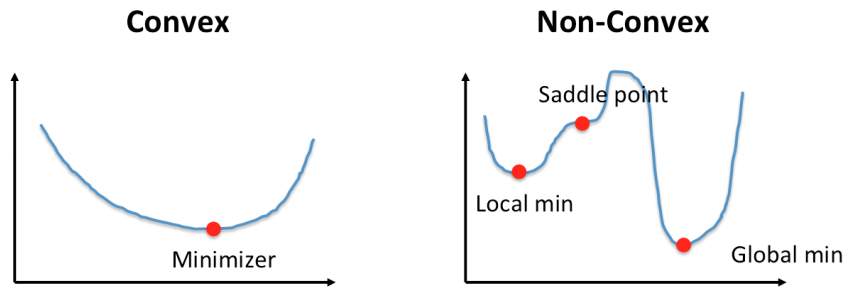
\includegraphics[width=0.8\linewidth]{ml/convexity.png}
        \caption{An illustration visualizing a convex function and a non-convex function. Also shown is the problem that comes with optimizing non-convex functions: getting stuck at a local minima.}
        \label{fig:convexity}
    \end{figure}
    
    Figure \ref{fig:convexity} illustrates this point. For the non-convex function, once you have reached a minimum, you don't know if it is a local minimum or a global minimum. However, in a convex function, you can be certain you have found a global minimum. Knowing that you are working with a convex optimization problem (i.e. a linear model) gives you the peace of mind in knowing that with enough training you will find weights that fit the data as well as possible for the model's complexity class.

\begin{questionbox}
\textbf{Synthesis Questions:}
\begin{enumerate}
    \item What does ``expressivity''  of a function mean?
    \item How do over and underfitting relate to bias and variance?
    \item If a model gives low bias and variance while fitting to a dataset, is it a good choice?
    \item Why is knowing that your optimization problem is convex useful/good?
    \item \textbf{Bonus:} Are either k-means or k-medians convex optimization problems? Give reasoning (does not need to be in proof form)
\end{enumerate}
\end{questionbox}

\section{When to Use Machine Learning Algorithms}
    \large Machine learning models are widely used in applications like image recognition, natural language processing, and predictive analytics. However, selecting the right algorithm for a task is essential. Simple models like linear regression may suffice for tasks with linear relationships, while more complex tasks (like image classification) often require more advanced models, such as neural networks.
    
    Furthermore, unsupervised learning methods like k-means clustering are valuable when you want to find hidden patterns in the data without labeled outcomes.

\section{Conclusion (ML)}
    \large This section covered the fundamental concepts of machine learning, with a focus on supervised learning (linear regression) and unsupervised learning (k-means clustering). We also introduced important concepts like regularization (L1 and L2), the bias-variance tradeoff, and convexity. Additionally, we discussed the differences between k-means and k-medians clustering and clarified why logistic regression is a classification algorithm. Understanding these basics is crucial as machine learning continues to influence more of our lives. These concepts are also the most applicable in day-to-day ML, the backbone of modern systems. More often than not, Occam's Razor holds true: Don't use more than necessary and overcomplicate things.


\section*{DEEP LEARNING}
\addcontentsline{toc}{section}{\protect\numberline{}DEEP LEARNING}
\section{Introduction to Neural Networks}
\subsection{Fundamental Structure}
\begin{flushleft}
    \large {To understand deep learning (DL) on a deeper level, we must first look closer at neural networks. They are ubiquitous in the space of DL and are the backbone or an integral part of most modern DL model architectures. As such, understanding what they are and where their ``power'' comes from is very important for both reasoning about the capabilities of DL systems and designing your own. \break
    
    Neural networks are learning algorithms loosely modeled after the brain. We will expand on this connection further in the future, but for now here are the basics: \textbf{Neurons} in the brain have lots of connections to other neurons, and can pass information between each other using electrical potentials shot down a long section of the cell called an \textbf{axon}. We \textit{heavily} abstract this complex biological process by representing it as a directed graph. We represent the neurons as nodes, and the axons as edges. \break
    
    The figure below shows how a graph like this might appear.}
    \begin{figure}[H]
        \centering
        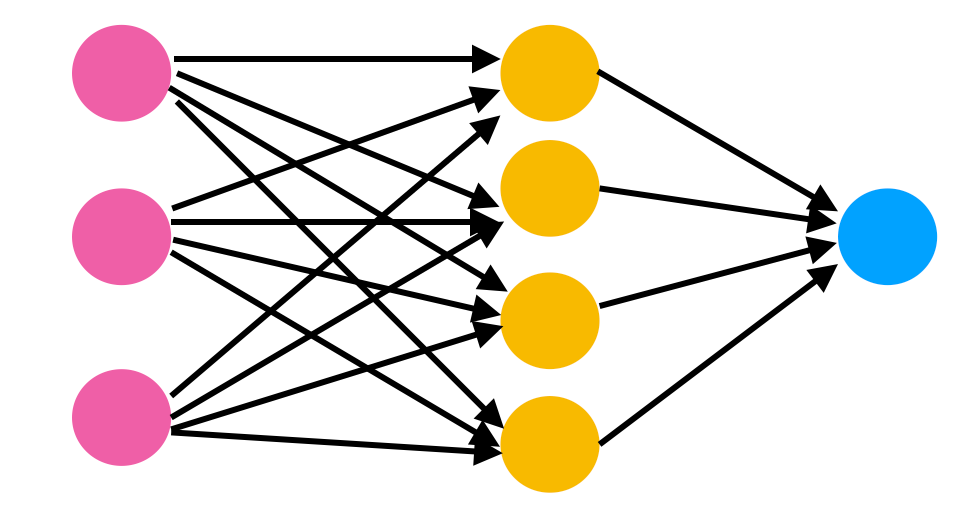
\includegraphics[width=0.5\linewidth]{dl/neuralnetwork.png}
        \caption{A visualization of neural networks}
        \label{fig:neuralnetwork}
    \end{figure}
\end{flushleft}

    \begin{flushleft}
    \large {As you can see in Figure 1 above, there are different levels or layers of neurons (pink, then yellow, and finally blue). That is a key characteristic of deep learning, a learning algorithm that uses \textbf{hierarchical layers to process information}. \break
    
    The primary layer of neurons is called the \textbf{input layer} - this is the layer where our input is read in as a vector. So if, for example, our input was an image (which is common as deep learning algorithms are often used for image classification), the image would be reconfigured into a large single-column vector, where each entry would represent a pixel in the image. The image would be, technically, entered into the model as one long vector of pixels, and this vector would be entered into the input layer of the model.}
    \end{flushleft}

\begin{figure}[H]
    \centering
    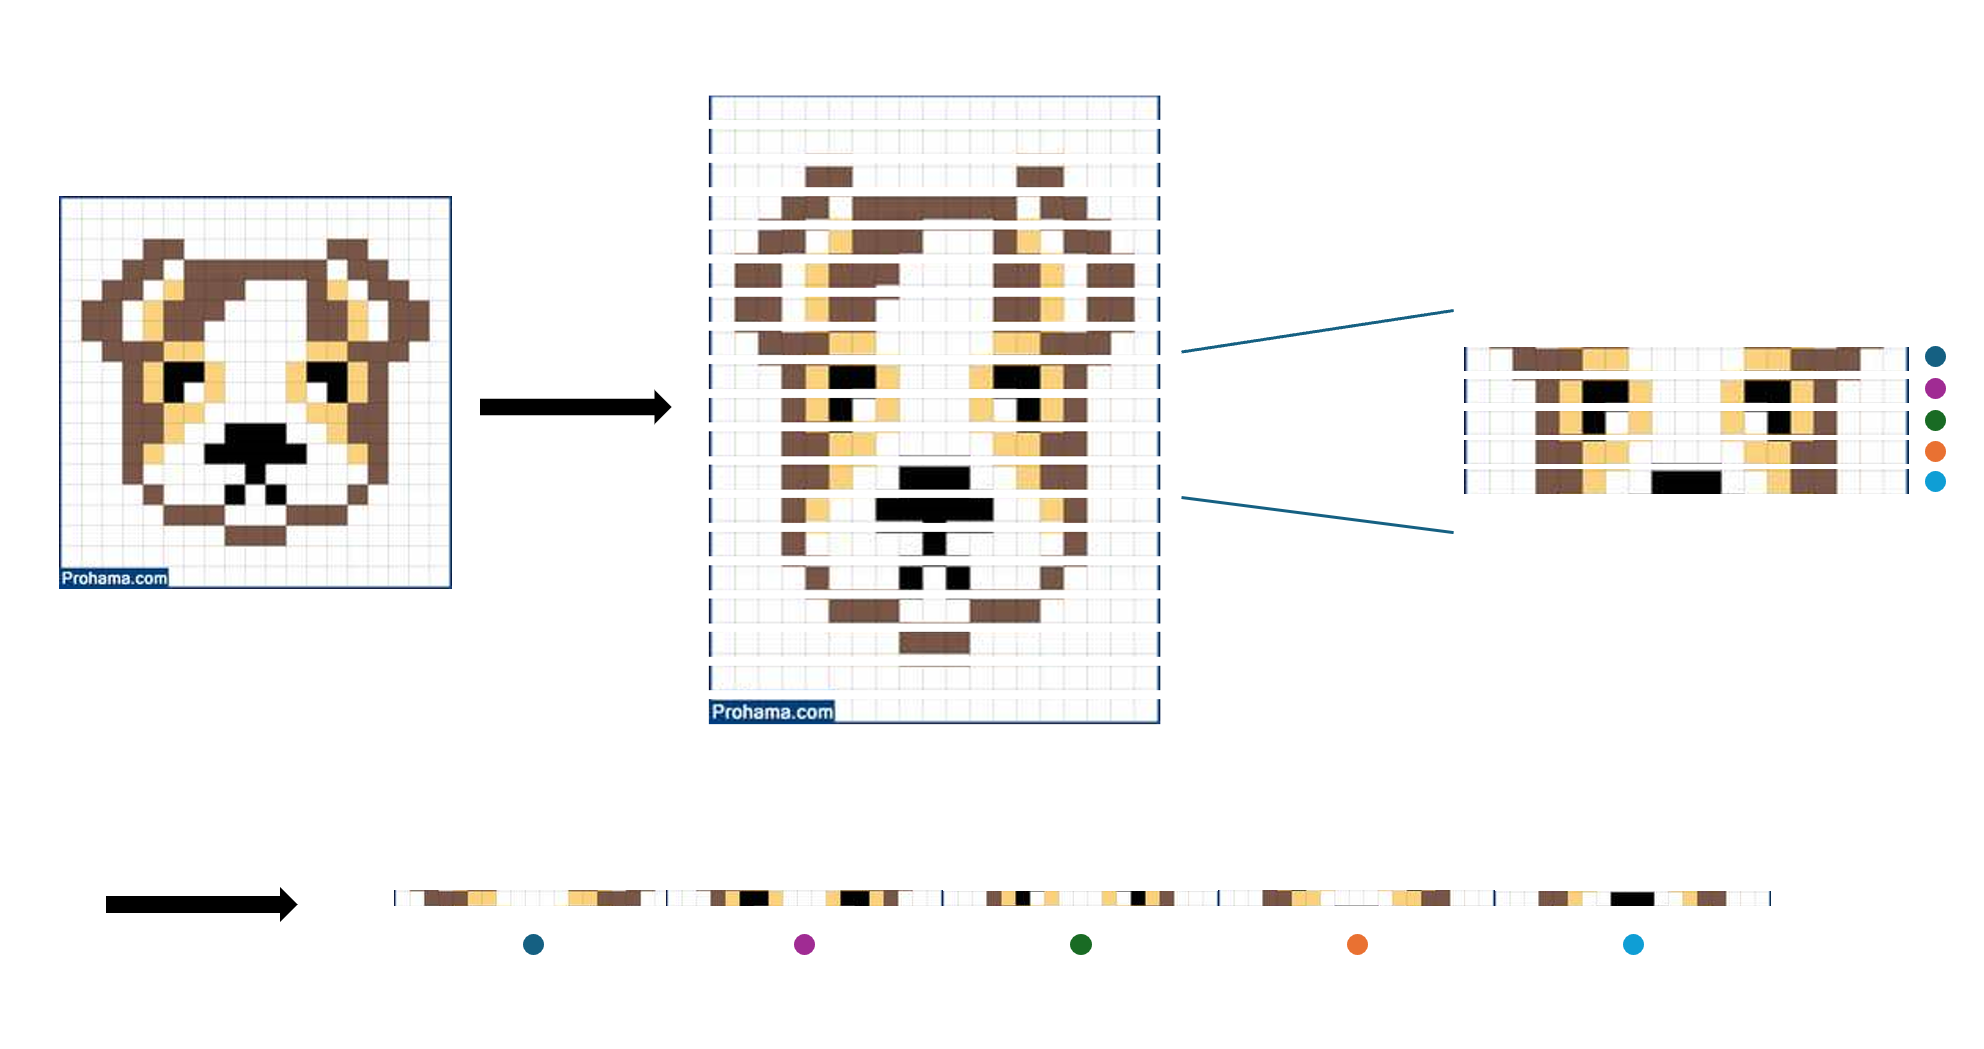
\includegraphics[width=1\linewidth]{dl/img-vector.png}
    \caption{Visualization of how images are converted into vectors}
    \label{fig:img-vector}
\end{figure}

\begin{flushleft}
    \large {Next are the \textbf{hidden layers}, which are yellow in the first image. There are usually multiple hidden layers in deep learning models, depending on how much processing the model must do before it can make a conclusion. The hidden layers are called ``hidden'' because we often don't understand what happens in here. Trying to interpret the vectors that exist in these layers usually results in nonsense. The field of explainable AI (XAI) has done lots of work here and there do exist tools to probe the hidden layers to understand what the model is ``thinking'' (I use the term thinking \textit{very} loosely here). However, without these tools, the middle of the network is considered a ``black box'' - a term you may have come across before. \break
    
    Finally, the \textbf{output layer}. The neural network calculates a probability for each possible outcome (for example, the input being an image of a dog) and fills out the output layer with values (blue in Figure 1). The output layer shows the algorithm's conclusions for the probabilities of each possible outcome and using these probabilities, the computer chooses an outcome. For classification neural networks, all the probabilities in the outcome layer will always add up to 1. Since there is one probability calculated for each outcome, the number of nodes in the output layer will be the number of possible outcomes. \break
    
    A small aside: Image inputs are the most common introduction to neural networks, because the ``Hello World'' project of deep learning, or the most introductory deep learning project, concerns image classification. It is important to note, however, that we could instead input ``features'' of some object we wish to classify or regress on. For example, we could provide the neural network with a vector consisting of the first index being the number of legs of an animal, the second index the height, the third a boolean indicating if it is a carnivore, etc. So, why don't we? \break
    
    A large reason neural networks are so useful is that they don't require too much ``feature engineering'' to get good results. Before the proliferation of the neural network, people would write complex algorithms to extract some features from an image. Where and how large the eyes of an animal are, an estimated number of legs, its edge contours, and many more complex features. They would then feed these vectors into a more traditional classification algorithm like a decision tree. \textbf{Neural networks are powerful enough that we can just cut up the raw image and throw it in. No complex engineering required!} This is why images are used in beginner projects: to demonstrate the power of these networks. However, this comes at the cost of efficiency. Neural networks often require orders of magnitude more data to train on, and also a lot more compute. The reasons for this will be explained in later sections.}
\end{flushleft}
\subsection{Flow of Information}
\begin{flushleft}
    \large Now that you understand the different layers of a neural network, let's see how the values in the input layer travel through the edges to get to the output layer. For ease of understanding, we are using a very simplified and weak version of a neural network, which we will improve in later sections. \break
    
    \textbf{Weights:} Zoom in one of the neurons in the input layer, and see how it connects to the next hidden layer. You will see one arrow pointing to each of the yellow neurons. Each of these arrows has a number attached to it. We call these numbers ``weights'' because they determine how much information from the previous node enters the next node. If you have a node with value $a$ connected to node $z$ with weight $w$, Node $z$ takes on the value of $a$ times $w$. If $w$ is very large or small, then this will heavily influence the value in $z$. If $w$ is closer to 0, then $z$ will not be influenced much by the value in $a$. You will also notice that one yellow neuron has multiple arrows going into it. This means multiple different neurons in the previous layer are sending their information over to this one. you just sum up the contributions. Nothing fancy there! \break
    
    \textbf{Biases:} Each neuron has a ``bias'' term that is added to its value. It can be positive or negative and make the neuron more ``sensitive'' to input. For example, a bias of +5 means that even if the values coming in from the previous layer to this neuron are generally negative, it is counteracted with a positive bias. Vice versa for negative biases. \break
    
    Let's write this all out: \break
    
    Have the three pink neurons be $a_1$, $a_2$, $a_3$. Only consider the top yellow neuron, and call it $z$. The arrow connecting $a_x$ to $z$ is called $w_x$. The bias for the neuron $z$ is $b$. 

    \begin{figure}[H]
        \centering
        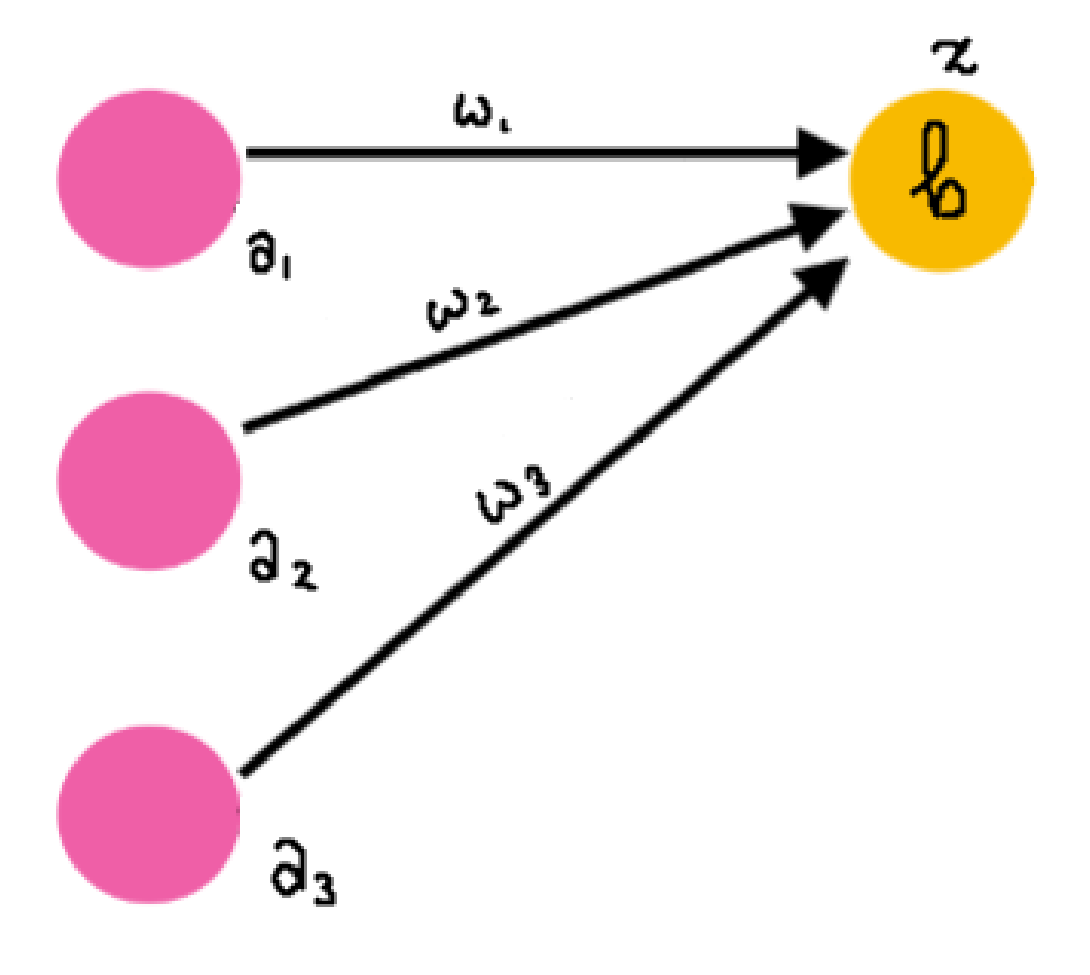
\includegraphics[width=0.5\linewidth]{dl/connectivity_basic.png}
        \caption{An illustration of weights and biases connecting the first layer of our neural network to the first neuron of the second (hidden) layer.}
        \label{fig:connectivity_basic}
    \end{figure}

    $$z = (w_1a_1 + w_2a_2 + w_3a_3) + b$$

    That is how information is propagated! This process is repeated for every neuron in the hidden layers, all the way out to the output layer. However, this is not done sequentially as shown above, but through the use of \textbf{matrices}.

    The \textbf{dot product} of two vectors of the same dimension $\textbf{a}$, $\textbf{b}$ is written as $\textbf{a} \cdot \textbf{b}$, and when expanded becomes:

    $$\sum_{i=1}^n a_ib_i$$

    Where $\textbf{a}$, $\textbf{b}$ $\in \mathbb{R}^n$. This is just saying that the vectors both have $n$ elements in them. We can rewrite the equation for $z$ as:

    $$z = \textbf{w}\cdot\textbf{a} + b$$

    We can add further subscripts to allow us to consider the whole hidden layer instead of one yellow neuron. Have the four yellow neurons be $z_1$, $z_2$, $z_3$, $z_4$. $\textbf{w}_x$ would then be a vector of the weights connecting the previous layer to $z_x$. We also add a subscript to the bias term to indicate which neuron in the hidden layer it belongs to. We now have, for the entire hidden layer:

    $$z_1 = \textbf{w}_1\cdot\textbf{a} + b_1$$
    $$z_2 = \textbf{w}_2\cdot\textbf{a} + b_2$$
    $$z_3 = \textbf{w}_3\cdot\textbf{a} + b_3$$
    $$z_4 = \textbf{w}_4\cdot\textbf{a} + b_4$$

    Using the properties of matrix multiplication (see \href{https://www.mathsisfun.com/algebra/matrix-multiplying.html}{here} if you need a refresher), we can simplify this further! We can define a \textbf{weight matrix} $W$ as a 4 $\times$ 3 matrix (4 rows, 3 columns):

    $$W = \begin{bmatrix}
            \textbf{w}_1\\
            \textbf{w}_2\\
            \textbf{w}_3\\
            \textbf{w}_4\\
            \end{bmatrix} = \begin{bmatrix}
                            w^1_1 & w^1_2 & w^1_3 \\
                            w^2_1 & w^2_2 & w^2_3 \\
                            w^3_1 & w^3_2 & w^3_3 \\
                            w^4_1 & w^4_2 & w^4_3 \\
                            \end{bmatrix}$$

    Making $\textbf{z}$ a vector holding all $z_x$ values and $\textbf{b}$ a vector holding all $b_x$ values, we can write:

    $$\textbf{z} = W\textbf{a} + \textbf{b}$$

    With the dimensions being: $\textbf{z} \in \mathbb{R}^{4 \times 1}$, $W \in \mathbb{R}^{4 \times 3}$, $\textbf{a} \in \mathbb{R}^{3 \times 1}$, and $\textbf{b} \in \mathbb{R}^{4 \times 1}$. Based on the architecture of your neural network, these numbers will change in expected ways.
\end{flushleft}

\subsection{The Perceptron and XOR}
\begin{flushleft}
    \large We just wrote out the equations that define how information flows between two layers in a neural network. Well, if we stop here and don't add any more layers, we come up with what is a \textbf{perceptron}. Understanding the limitations of two linear layers is crucial for appreciating the power of many nonlinear layers. Let us create a perceptron that accepts 2 inputs and outputs one.

    $$\textbf{z} = W\textbf{a} + \textbf{b}$$

    With the dimensions being: $\textbf{z} \in \mathbb{R}^{1 \times 1}$, $W \in \mathbb{R}^{1 \times 2}$, $\textbf{a} \in \mathbb{R}^{2 \times 1}$, and $\textbf{b} \in \mathbb{R}^{1 \times 1}$. Since the dimensions are so small, we can just do away with the compact matrix form:

    $$z = w_1a_1 + w_2a_2 + b$$

    $a_1$ and $a_2$ become $x$ and $y$ since we are in the Cartesian plane.

    $$z = w_1x + w_2y + b$$

    Subtract $b$:

    $$z - b = w_1x + w_2y$$

    Since $z$ and $b$ are constant, we have essentially written the standard form of a line! $w_1$, $w_2$, and $b$ define the line. Solving for $z$ tells you where the point $(x, y)$ lies in relation to the line. If $z$ is positive, the point lies above the line. 0 for on the line, and negative for below. \textbf{Therefore, the classification boundary a perceptron draws is linear.}

    What is this all for? Let's consider a famous problem: The XOR Problem. We construct a ``dataset'' from the definition of the XOR ($\oplus$) boolean function. The truth table for it can be seen below:

    $$\begin{array}{|c|c|c|}
    \hline
    X & Y & X \oplus Y \\
    \hline
    0 & 0 & 0 \\
    0 & 1 & 1 \\
    1 & 0 & 1 \\
    1 & 1 & 0 \\
    \hline
    \end{array}$$

    We can consider $X$ and $Y$ as Cartesian coordinates and $X \oplus Y$ as the ``class'' of the point. If this is plotted, you will quickly notice that \textit{there is no way to draw a line that cleanly separates the classes.} In other words, the XOR classification problem is \textbf{not linearly separable}.

    \begin{figure}[H]
        \centering
        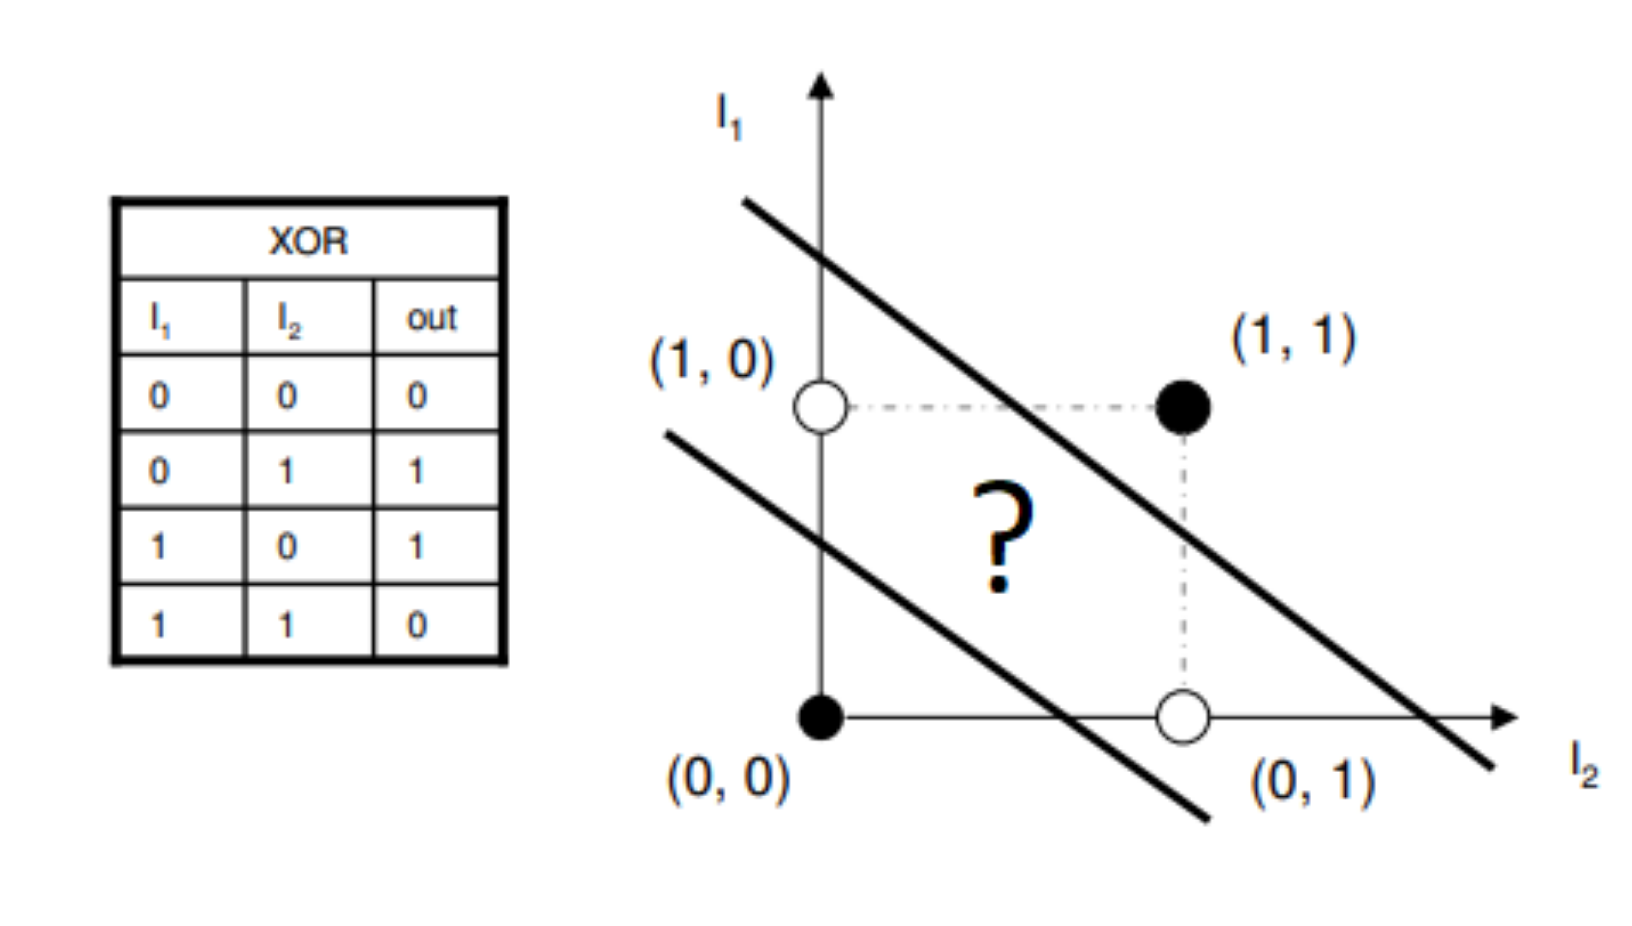
\includegraphics[width=0.5\linewidth]{dl/xor.png}
        \caption{Illustration of the XOR function, and how you cannot draw a single line that separates the classes (white and black dots).}
        \label{fig:xor}
    \end{figure}
    
    XOR is a simple boolean operation, as we move to complex problems like animal classification and speech recognition, how can perceptrons hope to solve them, even if we blow up the number of weights and nodes? You may say that we can add more layers, which can be represented as:

    $$\textbf{z}^1 = W^1\textbf{a} + \textbf{b}^1$$
    $$\textbf{z}^2 = W^2\textbf{z}^1 + \textbf{b}^2$$
    $$\textbf{z}^3 = W^3\textbf{z}^2 + \textbf{b}^3$$

    With superscripts just denoting what layer we are processing. Collapsing this set of equations through substitution:

    $$\textbf{z}^3 = W^3(W^2(W^1\textbf{a} + \textbf{b}^1) + \textbf{b}^2) + \textbf{b}^3$$

    Distribute:

    $$\textbf{z}^3 = W^3W^2W^1\textbf{a} + W^3W^2\textbf{b}^1 + W^3\textbf{b}^2 + \textbf{b}^3$$

    Here comes the issue with more layers. The term $W^3W^2W^1\textbf{a}$ can simply be collapsed into a single transformation $W\textbf{a}$! The decision boundary is still linear, and can therefore never ``solve'' a problem that is not linearly separable. The terms $ W^3W^2\textbf{b}^1 + W^3\textbf{b}^2 + \textbf{b}^3$ do not change this fact. Applying multiple linear transformations to a vector is the same as applying the product of those transformations all at once. The associative property of matrix multiplication totally allows this, since

    $$(AB)C = A(BC)$$

    Here is another way of looking at the above equation. See how the matrices can collapse into one?

    $$\textbf{z}^3 = (((W^3W^2)W^1)\textbf{a}) + W^3W^2\textbf{b}^1 + W^3\textbf{b}^2 + \textbf{b}^3$$
    
    Therefore we are back at square one as we were with two layers, just with more bias terms... So how do we make it so that we can draw more than just lines in our spaces to solve the XOR problem? The answer lies with nonlinearities (shocker!).
\end{flushleft}

\begin{questionbox}
\textbf{Synthesis Questions:}
\begin{enumerate}
    \item Define the following words:
    \begin{itemize}
        \item Neuron
        \item Layer
        \item Hidden Layer
        \item Weight
        \item Bias
    \end{itemize}
    \item If you have a neural network with an input dimension of 3, a hidden dimension of 4, and an output dimension of 1, then what would:
    \begin{itemize}
        \item The dimension of $W$ between the input and hidden layers be?
        \item The dimension of $W$ between the hidden and output layer be?
        \item The dimension of $\textbf{b}$ for the hidden layer?
    \end{itemize}
    \item Explain in your own words why a linear classifier (like a perceptron) cannot be used to solve the XOR problem
\end{enumerate}
\end{questionbox}

\section{Non-Linearity and Activation Functions}
\subsection{Introducing Nonlinearities}
\begin{flushleft}
    \large Let's take a step up from the XOR problem and look at something arguably more complex: Image classification. Image classification, especially with categories as specific as `dog' or `cat', is very challenging. It requires a level of detail and processing that many machine learning algorithms cannot achieve, especially linear algorithms, where a change in the input is directly proportional to the corresponding change in output. So, to tackle complex tasks such as image classification, neural networks, and deep learning models need to employ \textbf{non-linearity}. In non-linear models, changes in input can cause varying levels of change in corresponding output. Going back to our dog example, if we change the size of a dog's ear, we want that to have little impact on the model's conclusion. But if we change how the dog's fur appears, that should have a much larger impact. Non-linearity can help us achieve this. To introduce non-linearity to neural networks, models implement \textbf{activation functions}. \break
    
    Activation functions are applied after computing the raw values to populate the nodes of a neural network layer. These raw outputs are called \textbf{logits}. Recall Figure \ref{fig:neuralnetwork}. In the below equation, the values in the vector $\textbf{z}$ would be the logits of the hidden layer:

    $$\textbf{z} = W\textbf{a} + \textbf{b}$$

    This is NOT immediately what is passed to the final layer. Instead, we first apply a non-linear function to the logits. We can refer to this function as $\phi(\cdot)$, and we will give specific examples of this function later. Therefore, a multi-layer neural network (or in other words, a non-linear multi-layer perceptron) can be written out as follows:

    $$\textbf{z}^1 = \phi(W^1\textbf{a} + \textbf{b}^1)$$
    $$\textbf{z}^2 = \phi(W^2\textbf{z}^1 + \textbf{b}^2)$$
    $$\textbf{z}^3 = \phi(W^3\textbf{z}^2 + \textbf{b}^3)$$

    Now let's collapse this equation, and see if we run into the same problem we had with a multi-layer linear perceptron:

    $$\textbf{z}^3 = \phi(W^3\phi(W^2(\phi(W^1\textbf{a} + \textbf{b}^1) + \textbf{b}^2) + \textbf{b}^3)$$

    The matrices can no longer be collapsed into just one, meaning that we can \textit{draw more complex boundaries between classes, or find more complex patterns within regression tasks.} Using activation functions to allow for non-linearity gives deep learning and neural network models the strength to find solutions for complex tasks. A fundamental concept in the theory of neural networks, called the \textbf{Universal Approximation Theorem}, states that a neural network with at least one hidden layer with a finite number of neurons can approximate any continuous function to any level of accuracy with the use of certain activation functions. So, using non-linearity, neural networks can predict almost anything and do so accurately. Of course, we would also need enough data and compute to train this arbitrarily large model. \break
\end{flushleft}
\subsection{Common Activation Functions}

\begin{flushleft}
\begin{figure}[H]
    \centering
    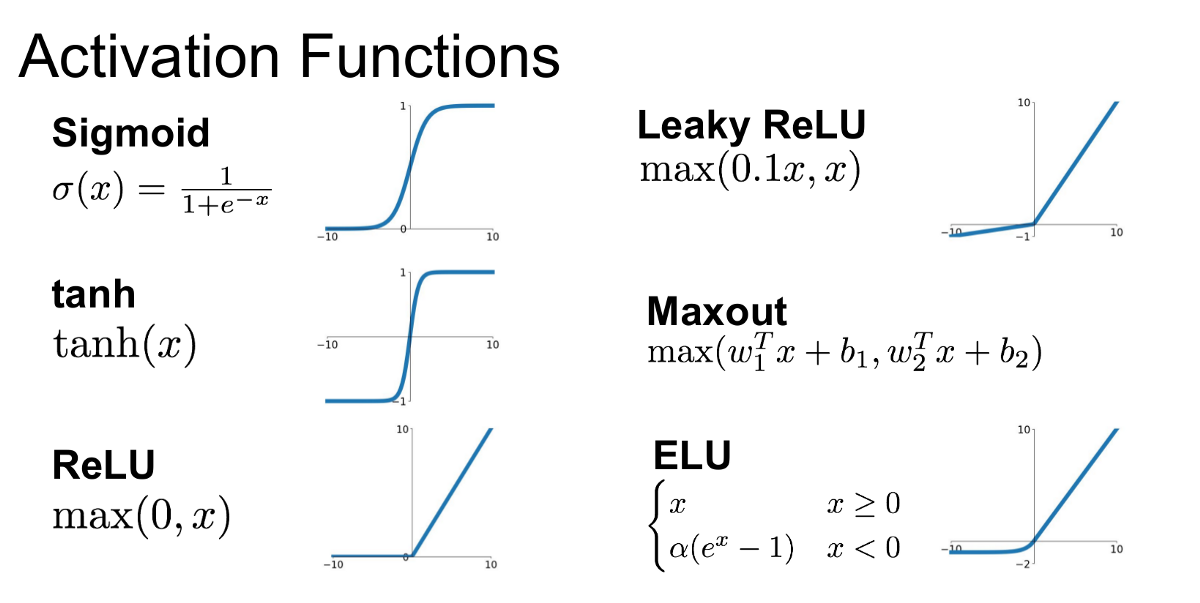
\includegraphics[width=0.75\linewidth]{dl/activationfuncs.png}
    \caption{Plots of various activation functions}
    \label{fig:activationfuncs}
\end{figure}
    \large One commonly used activation function is the \textbf{sigmoid function}. This function squashes inputs into the range between 0 and 1. It is useful in binary classification tasks but can cause issues like vanishing gradients in deeper networks (more on this later). The formula, where $x$ is a given neuron's output is:
    \begin{center}$\sigma(x) = \frac{1}{1+e^{-x}}$\end{center}
    The hyperbolic tangent activation function, or \textbf{tanh}, squashes inputs between -1 and 1. It is zero-centered, which makes it easier for optimization compared to the sigmoid function. The tanh formula is:
    \begin{center}$tanh(x) = \frac{e^x-e^{-x}}{e^x+e^{-x}}$\end{center}
    Another activation function, \textbf{Rectified Linear Unit or ReLU}, outputs the input if it's positive, and zero otherwise. It is computationally efficient and helps alleviate the vanishing gradient problem by allowing gradients to flow when the input is positive. ReLU is written as:
    \begin{center}$ReLU(x) = MAX(0,x)$\end{center}
    There is also another form of the ReLU activation function called \textbf{Leaky ReLU} that allows a small, non-zero gradient when the input is negative, helping prevent the issue of "dead neurons" (neurons that never activate). Leaky ReLU looks like:
    \begin{center}\[f(x)= 
        \begin{cases}
            x,& \text{if } x > 0\\
            0.01x,              & \text{if } x \leq 0
        \end{cases}
    \]\end{center}
\end{flushleft}

\begin{questionbox}
    \textbf{Synthesis Questions:}
    \begin{enumerate}
        \item Define the following words:
        \begin{itemize}
            \item Activation function
            \item Logits
        \end{itemize}
        \item Why are activation functions important for increasing the power of a neural network?
        \item In your own words, what is the Universal Approximation Theorem?
    \end{enumerate}
\end{questionbox}

\section{Backpropagation}
\subsection{Loss Functions}
\begin{flushleft}
    \large How does a neural network `learn' using training (a.k.a labeled) data? It uses a process called \textbf{backpropagation}. This process adjusts the weights assigned to connections between neurons and the biases assigned to nodes to improve the algorithm's accuracy. Imagine for a moment, that we are working with deep neural network classifying images as dog or cat. In this case, we will want to assign a higher weight to the feature `long tongue' because that is an important feature in determining whether something is a dog or a cat. To implement this functionality, the model will have a hidden neuron that ``lights up'' (has a high value) when the input animal image has a long tongue. This will significantly sway the model's decision-making process, increasing the probability of the image being a dog. In comparison, a neuron relating to the feature `fur color' might want to have a smaller weight connecting it to the next layer, because cats and dogs have similar fur colors and this feature isn't as important in differentiating between cats and dogs. The backpropagation process will slowly adjust these weights to be this way, leading to an excellent classifier. \break
    
    So how does backpropagation determine which weights and biases to manipulate? To understand that, we have to discuss \textbf{loss functions}. A loss function is used to measure how far off the network's predictions are from the actual target values. It provides a numeric value that represents the error in the prediction. Generally, higher loss means the model did not perform well, and vice versa. The goal of backpropagation is to reduce this loss by adjusting the weights in the network. A common example of a loss function is \textbf{Mean Squared Error (MSE)}, which is often used for regression tasks. The formula for MSE is:
    
    $$L = \frac{1}{N} \sum^{N}_{i=1} (y_i - \hat{y}_i)^2$$
    
    where $L$ is the loss, or the model's error, $y_i$ is the target-value (also known as the correct answer or label) for the specific input, $\hat{y}_i$ is the value the model predicted/guessed, and $N$ is the number of training examples shown to the model. You may notice that this version of the MSE loss function works only with scalar outputs from a neural network. There are versions of MSE that can handle multiclass output. However, it is generally accepted that if you have a multiclass classification problem, a better loss function to use is \textbf{Cross-Entropy Loss} (or log loss). This loss function measures the difference between two probability distributions. The formula for Cross-Entropy Loss is: 
    
    $$ L = -\frac{1}{N}\sum^{N}_{i=1} \sum^{K}_{k=1} y_{ik} \cdot log(\hat{y}_{ik})$$
    
    where $K$ is one of the outcomes or classes, $y_i$ is the actual probability of the given input belonging in class $K$, and $\hat{y}_i$ is the probability the model has assigned to class $K$ for the given input. \break
    
    Calculating these loss metrics is the final step of what is called the \textbf{forward pass}. This is what we have studied so far. After this begins the \textbf{backward pass} or \textbf{backpropagation}. 
\end{flushleft}

\subsection{Derivatives and Gradients}
\begin{flushleft}
    \large Before we delve into the semi-convoluted math behind backpropagation, we should revisit some concepts from calculus. Take a look at the equation and associated graph below:

    $$f(x, y) = z = x^2 + y^2$$

    \begin{figure}[H]
        \centering
        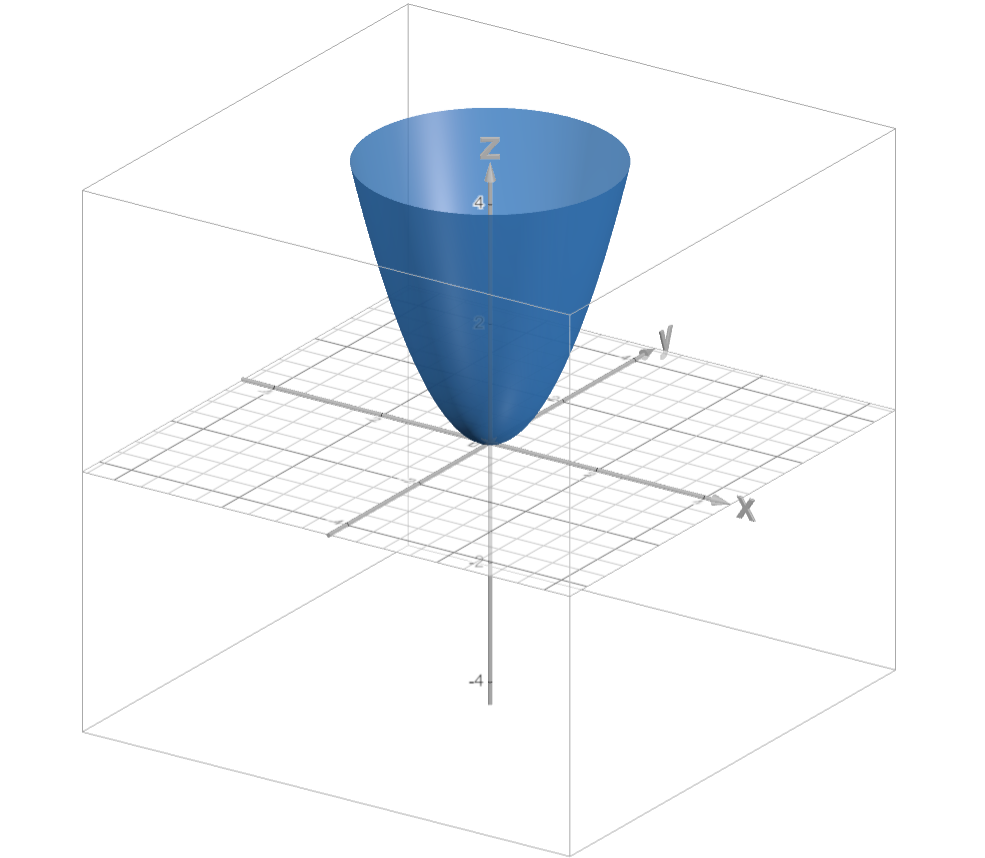
\includegraphics[width=0.5\linewidth]{dl/x2y2.png}
        \caption{Illustration of the function $f(x, y) = x^2 + y^2$}
        \label{fig:x2y2}
    \end{figure}

    The \textbf{gradient} of a multivariate function (denoted in this case as $\nabla f(x,y)$ or $\nabla z$) points you in the \textit{direction of steepest ascent} of a function given a point. To calculate the gradient of a function, you simply take the partial derivative of the function with respect to each variable and represent the derivatives as directions of a vector. Here is an example using $f(x,y) = z = x^2 + y^2$:

    $$\nabla z = \begin{bmatrix}
            \frac{\partial z}{\partial x}\\
            \frac{\partial z}{\partial y}\\
            \end{bmatrix}$$

    Solve for $\frac{\partial z}{\partial x}$:

    $$\frac{\partial}{\partial x}z = \frac{\partial}{\partial x}(x^2 + y^2)$$
    $$\frac{\partial z}{\partial x} = 2x$$

    Solve for $\frac{\partial z}{\partial y}$:
    
    $$\frac{\partial}{\partial y}z = \frac{\partial}{\partial y}(x^2 + y^2)$$
    $$\frac{\partial z}{\partial y} = yx$$

    $$\nabla z = \begin{bmatrix}
            2x\\
            2y\\
            \end{bmatrix}$$

    We now have a way to, given any point on the function, determine which direction to move to increase $z$ the most. If we plug in $(1,1)$, we get 
    
    $$\begin{bmatrix}
            2\\
            2\\
    \end{bmatrix}$$

    If we plot this as a vector on our previous graph:

    \begin{figure}[H]
        \centering
        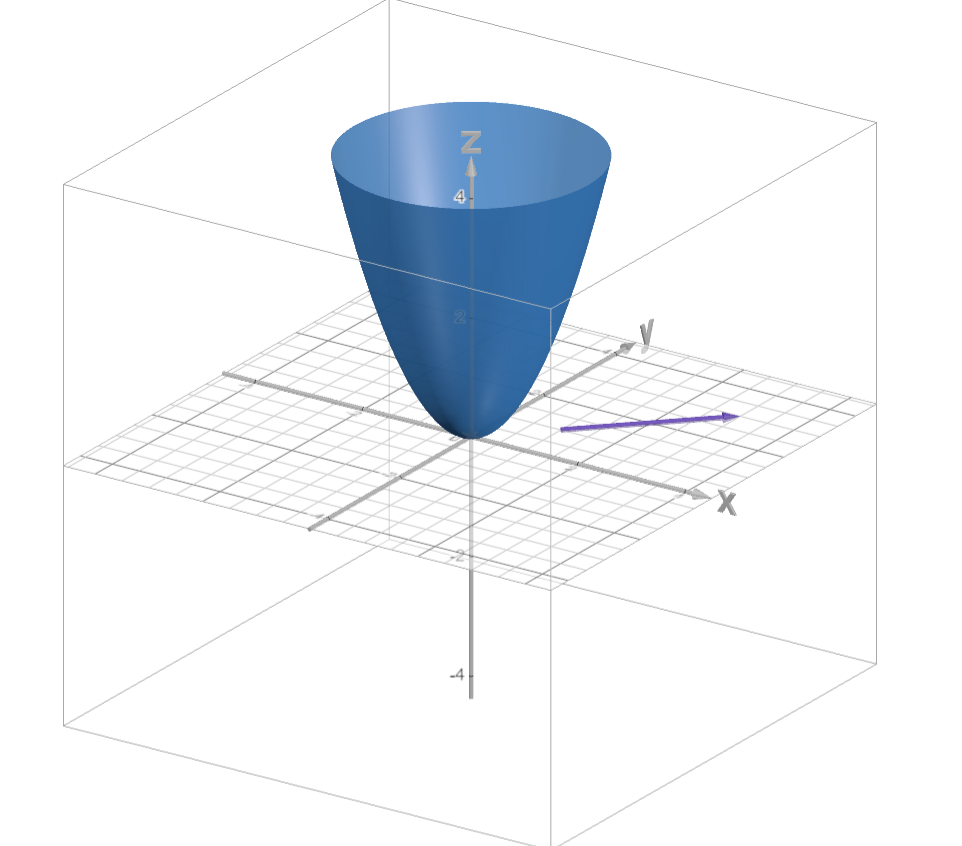
\includegraphics[width=0.45\linewidth]{dl/x2y2line.png}
        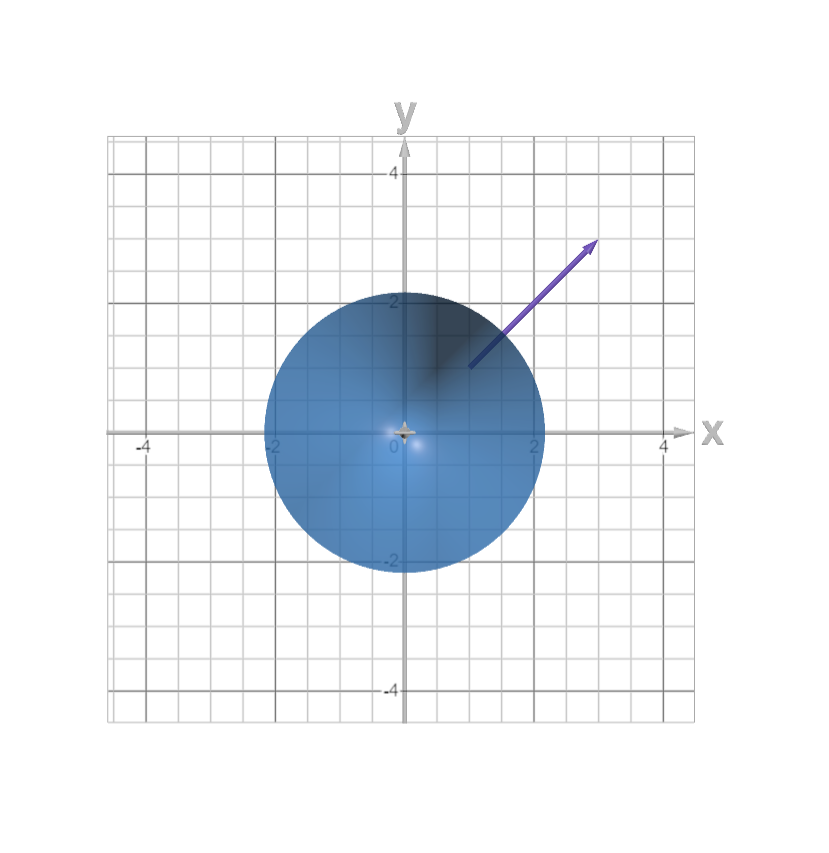
\includegraphics[width=0.45\linewidth]{dl/x2y2lineabove.png}
        \caption{Illustration of the function $f(x, y) = x^2 + y^2$, with a vector showing the direction of steepest ascent from point $(1,1)$}
        \label{fig:x2y2_2}
    \end{figure}

    So how does this relate to neural networks? Well, we can simply think of a neural network as a large multivariate function, with the variables in question being the weights. Think about it: we have a loss function that we want to reduce. We can imagine this as $z$ in the previous example. We want to find out how to change the weights to \textit{reduce} the loss function the quickest (direction of steepest descent). So, we just flip the idea of a gradient on its head. If we can find $\nabla_W L$ (the gradient of $L$ with respect to all weights), we can adjust the weights to minimize the loss!

    $$W_{new} \leftarrow W_{old} - \nabla_W L$$

    Calculating this by hand is near impossible, and nobody expects you to. There are tricks we can use to calculate gradients in chunks rather than taking 100's of derivatives.
\end{flushleft}

\subsection{Gradient Flow}
\begin{flushleft}
    \large The model first calculates the derivative of the loss with respect to $\hat{y}_i$, since $\hat{y}_i$ is the output of the model. For ease of understanding, we will use MSE loss:

    $$L = \frac{1}{N} \sum^{N}_{i=1} (y_i - \hat{y}_i)^2$$
    $$\frac{\partial}{\partial \hat{y}} L = \frac{\partial}{\partial \hat{y}}  \frac{1}{N} \sum^{N}_{i=1} (y_i - \hat{y}_i)^2$$
    $$\frac{\partial L}{\partial \hat{y}} =  \frac{1}{N} \sum^{N}_{i=1} -2(y_i - \hat{y}_i)$$

    This value is directly calculable, and it is propagated backward, starting ``gradient flow''. \break

    Lets say $\hat{y_i} = \sigma(z)$. Recall that $\sigma(\cdot)$ represents the \textbf{sigmoid} activation function. This therefore represents the activation function applied to the logits of the output neuron. \break
    
    Also define $z = f(w_1, w_2, ... w_n) = \sum_{i=1}^n a_iw_i + b$. Recall that $a_i$ is the output of neuron $i$ from the previous layer. This therefore represents the calculation of the output neuron's logits using the outputs from the neurons of the previous layer. \break
    
    % This is all visually represented in the image below:

    % \begin{figure}[H]
    %     \centering
    %     \includegraphics[width=0.5\linewidth]{}
    %     \caption{\todo{Create this image}}
    %     \label{fig:backpropviz}
    % \end{figure}

    How can we calculate $\nabla_W L = \biggl[ \frac{\partial L}{\partial w_1}, \frac{\partial L}{\partial w_2},...,  \frac{\partial L}{\partial w_n}\biggr]$? Using the chain rule, we can rewrite any $\frac{\partial L}{\partial w_x}$ as:

    $$\frac{\partial L}{\partial w_x} = \frac{\partial L}{\partial \hat{y}}\cdot\frac{\partial \hat{y}}{\partial z}\cdot\frac{\partial z}{\partial w_x}$$
    
    where $\frac{\partial L}{\partial w_x}$ is the gradient of the loss with respect to an arbitrary weight $w_x$, $\frac{\partial L}{\partial\hat{y}}$ is the gradient of the loss with respect to the predicted output, $\frac{\partial\hat{y}}{\partial z}$ is the gradient of the output with respect to the weighted sum $z$, and $\frac{\partial z}{\partial w}$ is the gradient of the weighted sum with respect to the weight $w$. \break

    We already have $\frac{\partial L}{\partial\hat{y}}$ as shown above. $\frac{\partial \hat{y}}{\partial z}$ is calculated as such:

    $$\hat{y_i} = \sigma(z)$$
    $$\frac{\partial}{\partial z}\hat{y_i} = \frac{\partial}{\partial z} \sigma(z)$$
    $$\frac{\partial \hat{y_i}}{\partial z} = \sigma'(z)$$

    $\sigma'(z)$ is just the derivative of the sigmoid. This is easy to compute. Calculating $\frac{\partial z}{\partial w_x}$ is a little harder, as we have considered $w_x$ as an arbitrary weight. Let us calculate the partial derivative with respect to just $w_1$. Calculating the other $w$ follows easily. \break

    $$f(w_1, w_2,...,w_n) = z = \sum_{i=1}^n a_iw_i + b$$
    $$\frac{\partial}{\partial w_1}z = \frac{\partial}{\partial w_1}\sum_{i=1}^n a_iw_i + b$$
    $$\frac{\partial z}{\partial w_1} = a_1$$

    It follows that $\frac{\partial z}{\partial w_2} = a_2$, $\frac{\partial z}{\partial w_3} = a_3$, and so forth. Therefore we can say that $\frac{\partial z}{\partial w_x} = a_x$. We can plug all these results into our chain rule:

    $$\frac{\partial L}{\partial w_x} = \frac{\partial L}{\partial \hat{y}}\cdot\frac{\partial \hat{y}}{\partial z}\cdot\frac{\partial z}{\partial w_x}$$
    $$\frac{\partial L}{\partial w_x} =  (\frac{1}{N}\sum^{N}_{i=1} -2(y_i - \hat{y}_i)) \cdot (\sigma'(z)) \cdot (a_x)$$

    For deeper neural networks with many layers, this computational graph becomes much more complex. However, the idea stays the same: Find the gradients of the loss with respect to the weights of each layer. Do this by passing gradients backward through the network. Calculating the gradient with respect to the biases is done the same, and even simpler! Performing gradient descent is then as simple as the equation from before, with a small constant added to ensure these changes are incremental and not massive:

    $$W_{new} \leftarrow W_{old} - \lambda\nabla_W L$$

    This constant $\lambda$ is called the \textbf{learning rate}, and we will discuss its significance later. Congratulations, you know understand basic gradient descent!
\end{flushleft}

\subsection{Optimizers and Learning Rates}
\begin{flushleft}
    \large While gradient descent is a common optimizer and is easy to follow mathematically, it is unfortunately very expensive computationally and can be slow. \textbf{Stochastic Gradient Descent (SGD)} is a similar, more efficient, optimizer. SGD speeds up this process by updating weights after computing the gradient on a small, random batch of data, rather than the entire dataset. Another popular optimizer is \textbf{Adam}. Adam combines the benefits of both SGD and another optimization technique called \textbf{Momentum}, which helps the optimizer move faster by incorporating information from past gradients. Adam also adapts the learning rate for each weight based on how the gradients change, making it efficient for handling noisy gradients and sparse data. Many people use Adam because it performs well across a wide range of tasks. It is essential to understand that Adam fine-tunes the learning process dynamically, making it more flexible than standard SGD. A deep dive into how each of these optimizers work is a bit beyond the scope of this article, but is interesting and I suggest you do some independent research! \break
    
    A common thread between all of these optimizers is that they share one parameter in common: the \textbf{learning rate}. This is a scaling factor applied to the calculated gradient before it is used to adjust the weights. The size of this scaling determines how big of a ``step'' the weights take while traversing the ``loss landscape''. Optimizer classes in most deep learning libraries (e.g. PyTorch, Tensorflow) have defaults that work well for each of the different optimizers. Starting here is usually a good idea, because a learning rate that is too small will take way too long to converge, while a large learning rate may not converge at all! For an illustration of this, see Figure \ref{fig:lr}.

    \begin{figure}[H]
        \centering
        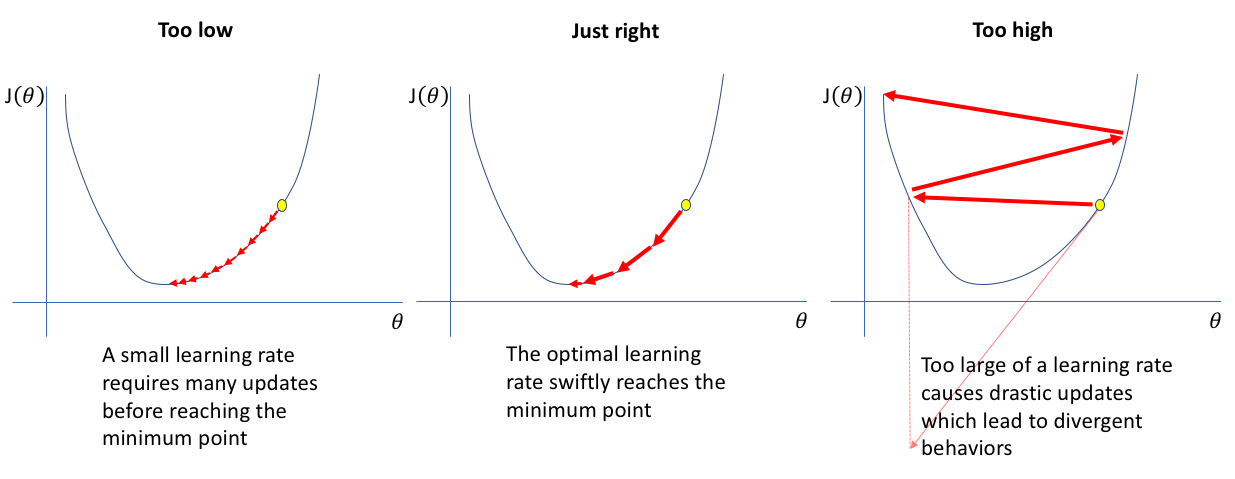
\includegraphics[width=1\linewidth]{dl/lr.png}
        \caption{A demonstration of how different learning rates affect convergence of a loss function (in this graphic represented as $J(\theta).$}
        \label{fig:lr}
    \end{figure}
\end{flushleft}

\begin{questionbox}
    \textbf{Synthesis Questions:}
    \begin{enumerate}
        \item Define what the purpose of a loss function is
        \item What are the different use cases for Mean Squared Error vs. Cross Entropy Loss?
        \item What is the difference between a derivative and a gradient?
        \item Find the gradient for this function at $(3, 2, 1)$:
        $$f(x,y,z) = \frac{2}{3}x^2 + y^2 - 2y + z^4 - \frac{4}{3}z^3$$
        \item Find the derivative of the sigmoid ($\sigma$) function and plot it. Why might this activation function prevent gradients from flowing back through the network during the backward pass?
        \item Why might the ``steps'' taken by SGD not be as directly in the most optimal direction compared to GD?
    \end{enumerate}
\end{questionbox}

\section{Regularization}
\begin{flushleft}
    \large We will now cover an incredibly important topic for deep learning: \textbf{regularization}. In ML, regularization often is applied in the form of adding a norm to the loss function, encouraging weights to reach smooth (L2) or sparse (L1) optima. Regularization also exists in deep learning to prevent overfitting, but comes about in more interesting and varied ways. We will quickly cover two common ones in shallow detail.
\end{flushleft}

\subsection{Dropout}
\begin{flushleft}
    \large \textbf{Dropout:} During each forward pass, a certain fraction of neurons are temporarily dropped from the neural network. The connections they have to other neurons are totally ignored and they are not used in the forward nor the backward pass for that specific training example. In other words, dropped neurons have no direct bearing on the output and their associated weights will not change from that training example. This only occurs at train time. At test time, all neurons are allowed to be used by the network all the time. See Figure \ref{fig:dropout} for a visual representation of this process.

    \begin{figure}[H]
        \centering
        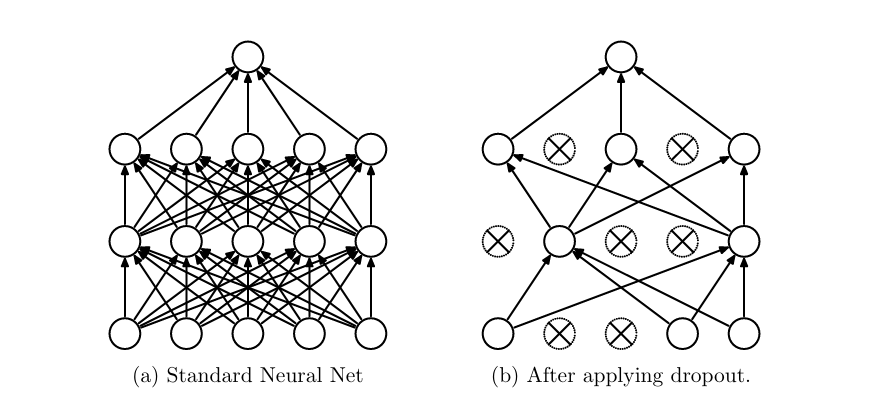
\includegraphics[width=1\linewidth]{dl/dropout.png}
        \caption{Visualizing dropout in a fully connected neural network}
        \label{fig:dropout}
    \end{figure}

    Why would we do this? Well, if a network is allowed to use all of its neurons all of the time, there is no guarantee that the network will \textit{effectively} use all the neurons. Perhaps due to a strange initial weight configuration, the random seed, or some other factor, the network will only use a very small subset of its available power. Many neurons will end up going essentially unused and their weights meaningless, despite the resources being allotted to train them. This consolidation of computation into a small portion of the network leads to much lower robustness. \break
    
    Here is an analogy: a 10-armed robot is trained to pick up an apple from a desk. The robot uses one of its arms at random, and only trains with that arm. Then during test time, we bind the arm the robot used the most. Since the robot has not learned how to use any of its other arms, it fails at a task it should very easily be able to do. Dropout is like forcing the robot to pretend it has lost a few arms each training example. It is then forced to use all of its arms, and gets good at picking up the apple with any of them. This robot is now much more robust when deployed into the real world, as small perturbations do not totally handicap it. \break

    One small detail is that once training time is over, all neurons have their weights scaled by 1 minus the dropout rate. Therefore, the expected distribution of values flowing from one layer to the next stays the same as it was during training time.
\end{flushleft}

\subsection{Batch Normalization}
\begin{flushleft}
    \large \textbf{Batchnorm:} Batchnorm, or batch normalization, is a very common technique used to regularize neural networks and improve training efficiency. Batchnorm can be thought of as an extra layer in a neural network with a few additional parameters. Essentially, before information flows from one layer to the next, the data is \textbf{normalized} across examples in the batch. Let's break this down. \break
    
    What is a \textbf{batch}? It is common to not just pass one example through a neural network at a time, but many. Groups of 64, 1024, 4096, etc. training examples are used at once before a backward pass is performed. Then what is \textbf{normalization}? Within this aforementioned batch, examples are mean-shifted by a mean $\mu$ and then divided by a standard deviation $\sigma$. This is normalization and it keeps the data centered around $(0,0)$ and evenly varied. In addition, these $\mu$ and $\sigma$ parameters are slightly adjusted for each new batch by taking a moving average through each previous batch. There are also additional ``scale and shift'' parameters represented by $\gamma$ and $\beta$ respectively. As the network sees more and more examples, the $\beta$ and $\gamma$ parameters are also slowly adjusted to find a scale and shift transformation to the normalized data that improves performance. This is shown in the following series of equations, where $x_i$ is a datapoint and $m$ is the number of datapoints in a batch. \break

    Estimating $\mu$ and $\sigma$ for a batch:
    $$\mu_{batch} = \frac{1}{m}\sum_{i=1}^m x_i$$
    $$\sigma_{batch} = \sqrt{\frac{1}{m}\sum_{i=1}^m (x_i - \mu_{batch})}$$
    Updating the moving average:
    $$\mu = \alpha \mu + (1-\alpha)\mu_{batch}$$
    $$\sigma = \alpha \sigma + (1-\alpha)\sigma_{batch}$$
    Normalize $x_i$ to $\Tilde{x}_i$ using the moving average:
    $$\Tilde{x}_i = \frac{x_i - \mu}{\sigma}$$
    Scale and shift before sending values to next layer:
    $$x_i^{output} = \gamma\Tilde{x}_i + \beta$$
    
    Mean-centered and evenly varied data allows gradient descent to descend the weights smoothly down to a optimal minimum. If two features input into a neural network were on wildly different scales (e.g. House price vs. number of bedrooms), then optimization becomes clunky. Making a large shift in weights is necessary to process highly varied housing prices, but this same shift negatively affects how the network processes the more tame ``number of bedrooms'' feature since more precise changes are needed. Normalization plus scale and shift removes this problem, and thus batchnorm helps greatly with a network's convergence.
\end{flushleft}

\begin{questionbox}
    \textbf{Synthesis Questions:}
    \begin{enumerate}
        \item In your own words, why does Dropout work?
        \item Why do you think a moving average of $\mu$ and $\sigma$ are useful for a network with batch normalization layers if there are many batches to process?
        \item Think of, or find online, a method of regularization within neural networks not discussed here. Write two to three sentences on how it works.
    \end{enumerate}
\end{questionbox}

\section{When to Use Deep Learning/Neural Networks}
\begin{flushleft}
    \large While we have shown the great power and ability of neural networks and deep learning, with all this power comes great cost. Neural networks are power-hungry, taking up significant computation power for all the processing they have to do. They are a powerful tool and should be used with caution and respect. As our i2 president once said, \textbf{don't use a bomb to cut a sandwich}. It is important to know when to use them. Deep learning models are useful for image, audio, and video classification or, in other cases, where non-linearity is necessary. Neural networks also require considerable amounts of data for a decent accuracy. Only use them when you have enough labeled data to properly train them on. In summary, while neural networks offer unmatched capabilities for complex tasks like image and audio classification, they are not always the most efficient tool. Sometimes a simpler model will get the job done while using half the resources. The key is understanding when their power is necessary and when a more lightweight solution will suffice. Always choose the right tool for the job.
\end{flushleft}

\section{Conclusion (DL)}
\begin{flushleft}
    \large This section covered the fundamental concepts of deep learning, with a heavy focus on neural networks. We also introduced important concepts like non-linearity and backpropagation. We closed with an overview of regularization techniques used in deep learning today. There is much more to deep learning we could not cover in this article. Neural networks especially are heavily used in many fields; either in larger deep learning architectures or as function approximators for some other goal. Understanding how they work and how to train them is critical to evaluating these systems. \break
\end{flushleft}

\section*{COMPUTER VISION}
\addcontentsline{toc}{section}{\protect\numberline{}COMPUTER VISION}
\section{Introduction to Computer Vision}
\subsection{What is Computer Vision?}
\begin{flushleft}
    \large \textbf{Computer vision} is a field of machine learning that focuses on enabling computers and programs to \lq see' images. \lq Seeing', in this case, defines a computer's ability to recognize and understand objects in images, such as a program \lq seeing' a dog and labeling it as such. Computer vision is used in many ways, most commonly utilized for \textbf{object detection, image classification, and segmentation} (a process of breaking an image down to identify boundaries of objects and objects themselves).  We will primarily be covering where computer vision instersects with deep learning, but do note that computer vision as a field has existed well before deep learning and there are many aspects of the field that are more algorithm based than AI based.
\end{flushleft}

\section{Convolutional Neural Networks}
\begin{flushleft}
    \large Now what machine learning algorithm is used for computer vision? That would be \textbf{Convolutional Neural Networks} or \textbf{CNNs}. CNNs are designed to process images and can either be found as independent models or as parts of other neural networks. They can work as image pre-processors for other models, like multimodal language models. Similar to how neural networks were designed to mimic brain functionality, CNNs are designed to \textit{mimic a human's visual processing system} and the brain's visual cortex. 

    \subsection{Convolutional Layer}
        Convolutional neural networks are structured as a series of layers, similar to neural networks. The first layers are called the \textbf{convolutional layers}. Convolutional layers apply a mathematical calculation to a section of an image to extract information about the features in that image. Recall that a feature is an attribute of interest, such as an ear, number of legs, presence of color, etc. It does this using an object called a \textbf{kernel}. A kernel works like a sort of filter, amplifying the effect of some pixels and minimizing the effect of others to try and draw out a feature. For example, the kernel in the image below is attempting to extract an ``ear'' feature from a section of the input image. 
        \begin{figure}[H]
            \centering
            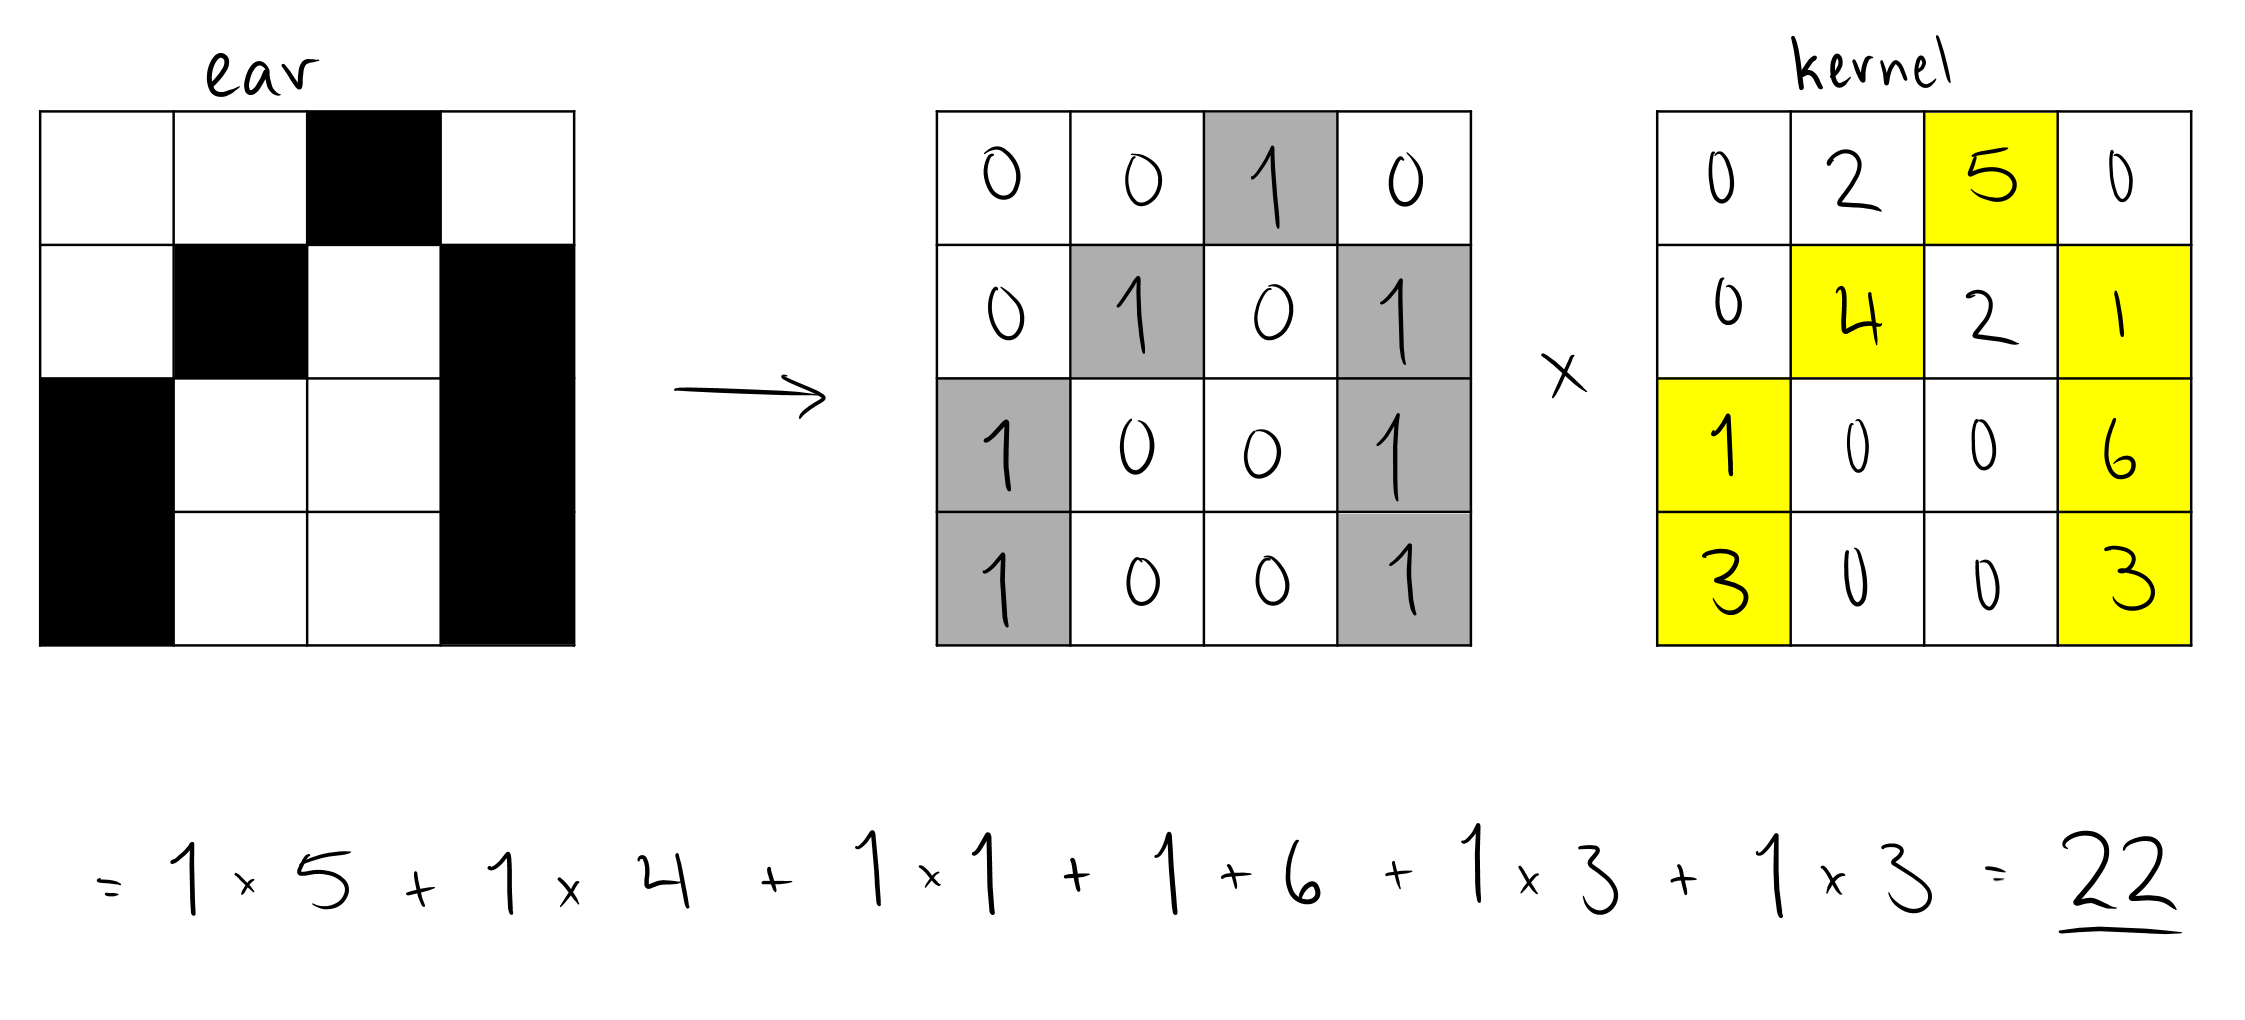
\includegraphics[width=1\linewidth]{cv/kernelextraction.png}
            \caption{Illustration of feature extraction using kernel}
            \label{fig:kernelextraction}
        \end{figure}

        The solution to the calculation is then placed back into a new, usually smaller, matrix that will ultimately become a representation of where the features we are searching for within the image exist. We call this a \textbf{feature map}. For example, if there is an ear in the top left of an image, then an ``ear'' kernel applied to that image will result in a feature map that has high values in the top left where the ear was. 

        \begin{figure}[H]
            \centering
            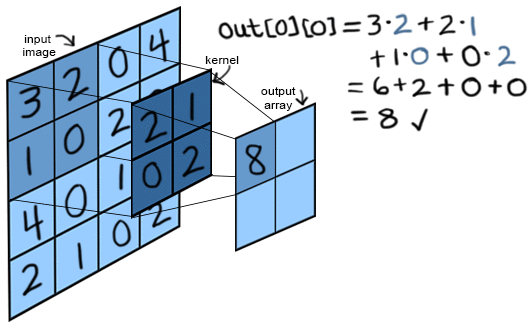
\includegraphics[width=0.75\linewidth]{cv/imagetokerneltosmallmatrix.png}
            \caption{Illustration of the work done in a convolutional layer}
            \label{fig:imagetokerneltosmallmatrix}
        \end{figure}

        The formula for the convolutional layer's calculation is a dot product calculation, where a filter (a.k.a kernel) $F$ is applied to an image in sections (the number of sections depends on the size of the image and the size of the filter) as seen below. We will use the image above for examples as we break down the equation.
        
        $$Z(i, j) = \sum^{k-1}_{m=0} \sum^{k-1}_{n=0} \sum^{C}_{c=1}  I(i+m, j+n, c) \cdot F(m, n, c) $$
        
        The variables $i$ and $j$ denote where in the image we are looking at the moment. If we input $(0,0)$, the top left of the filter would be placed at $(0,0)$. This is what is happening in the above figure. \break
        
        The size of the filter is an $k \times k$ matrix (a $2 
        \times 2$ matrix in the above figure). So when we place it on the image, we get an $k \times k$ ``focus zone'' where we are looking for a feature. \break
        
        $m$ and $n$ within the summations denote the coordinates of pixels in both the image $I$ and the filter. We iterate through them, multiplying the pixel value of a coordinate within the image by the value within the filter that ``overlaps'' it. You can see this being done in the above image, as we multiply the pair $3 \times 2$. The 3 comes from the image and the 2 comes from the overlapping spot in the filter. We repeat this for all pixels in the ``focus zone'', summing them all up.\break
        
        The coordinate $c$ designates the \textbf{channel} of the image and filter the calculation is currently focusing on. Colored images have 3 channels, one that stores the R (red) pixel value, one that stores the G (green) pixel value, and one that stores the B (blue) pixel value. We would apply a filter to each of these channels separately. This allows us to detect features through the dimension of color as well (e.g. ``red ear''). The filters applied to each channel can be the same, or different, depending on the architecture of the CNN. There are also other encodings for colored images, such as HSV or CMYK. Black and white images can be encoded in just one channel.\break
        
        Finally, $Z(i,j)$ returns the value  that we will store in the feature map described previously. \break

        Along with kernels, two other factors affect how the feature map $Z$ is created, \textbf{stride} and \textbf{padding}. Stride denotes how many pixels the filter is shifted by during the calculation. The kernel can be shifted by only 1 pixel meaning there will be overlap in the sections of the image the kernel is placed on. Or, with a stride that equals the width of the kernel, the sections that the kernel is applied to do not overlap. In the above image, the stride is 2. Observe more examples of strides that are depicted in Figures 3 and 4 below. 

        \begin{figure}[H]
            \centering
            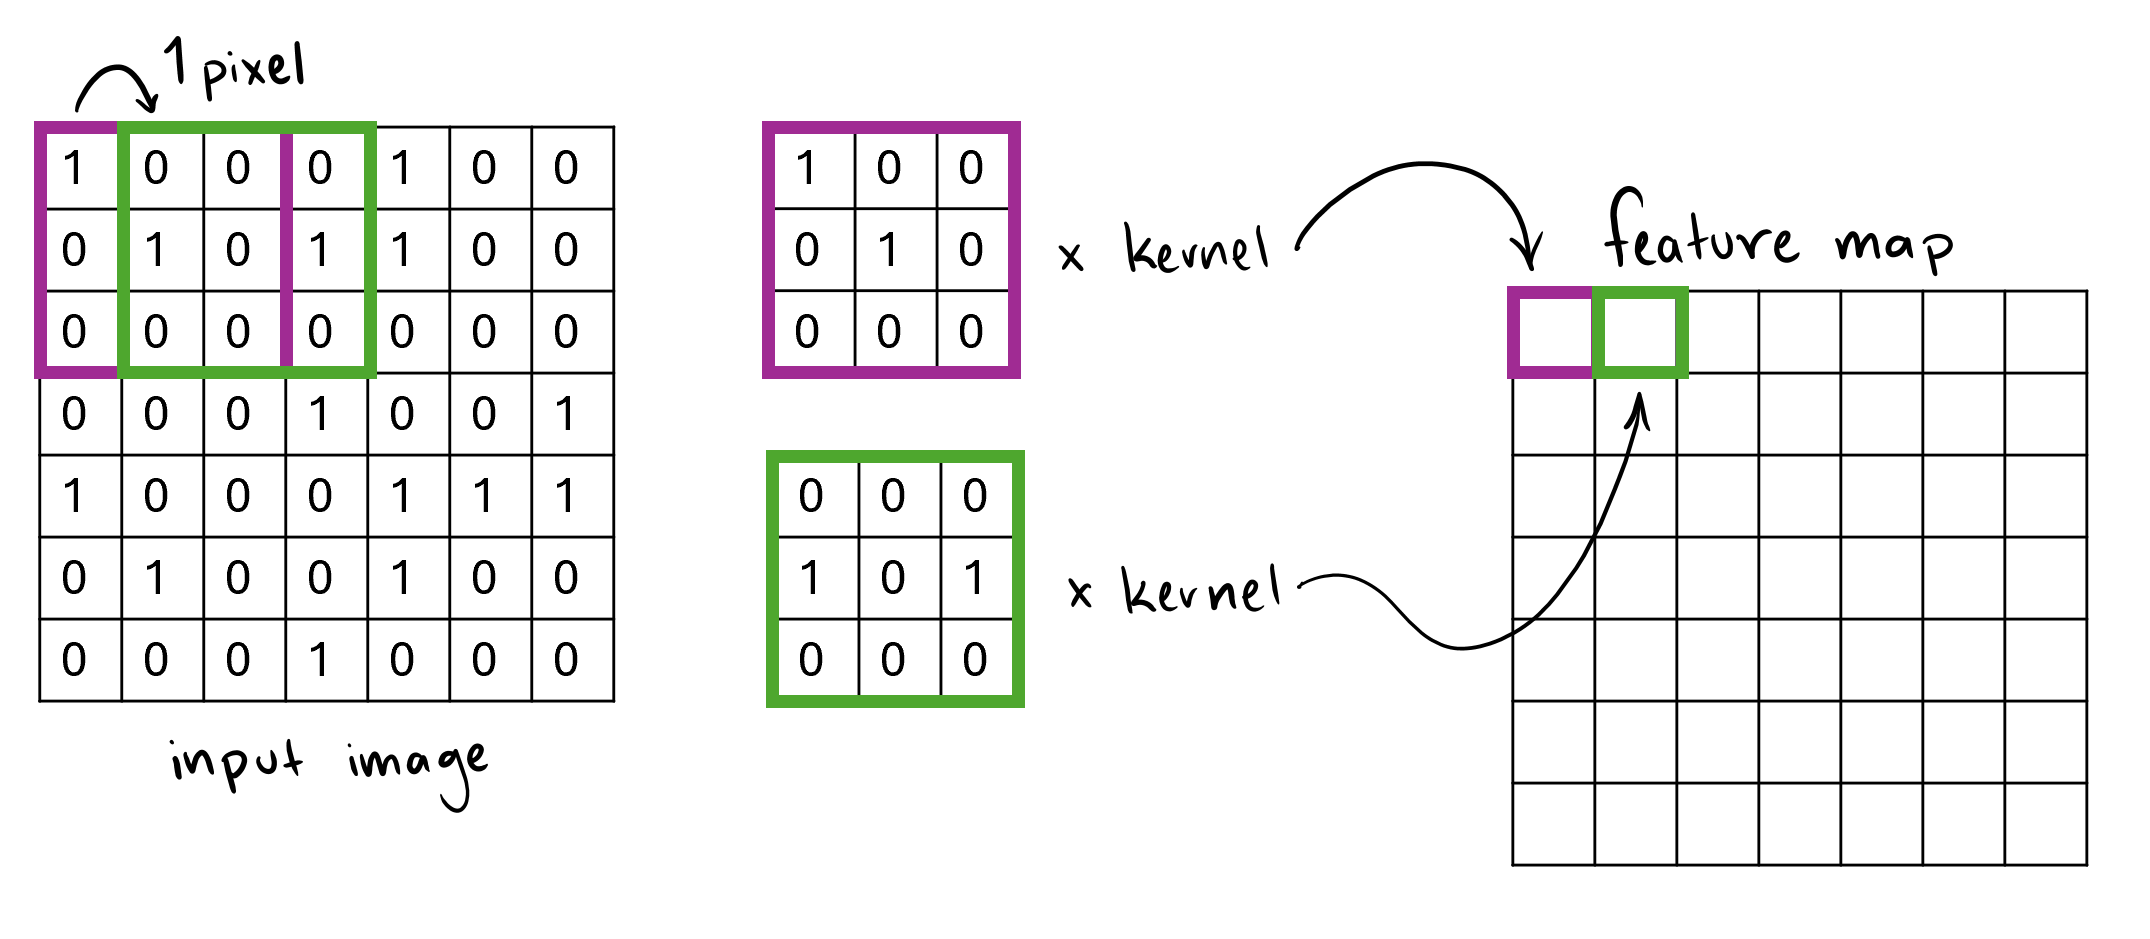
\includegraphics[width=1\linewidth]{cv/stridedepict.png}
            \caption{Illustration depicting a stride of 1 pixel}
            \label{fig:stridedepict}
        \end{figure}

        \begin{figure}[H]
            \centering
            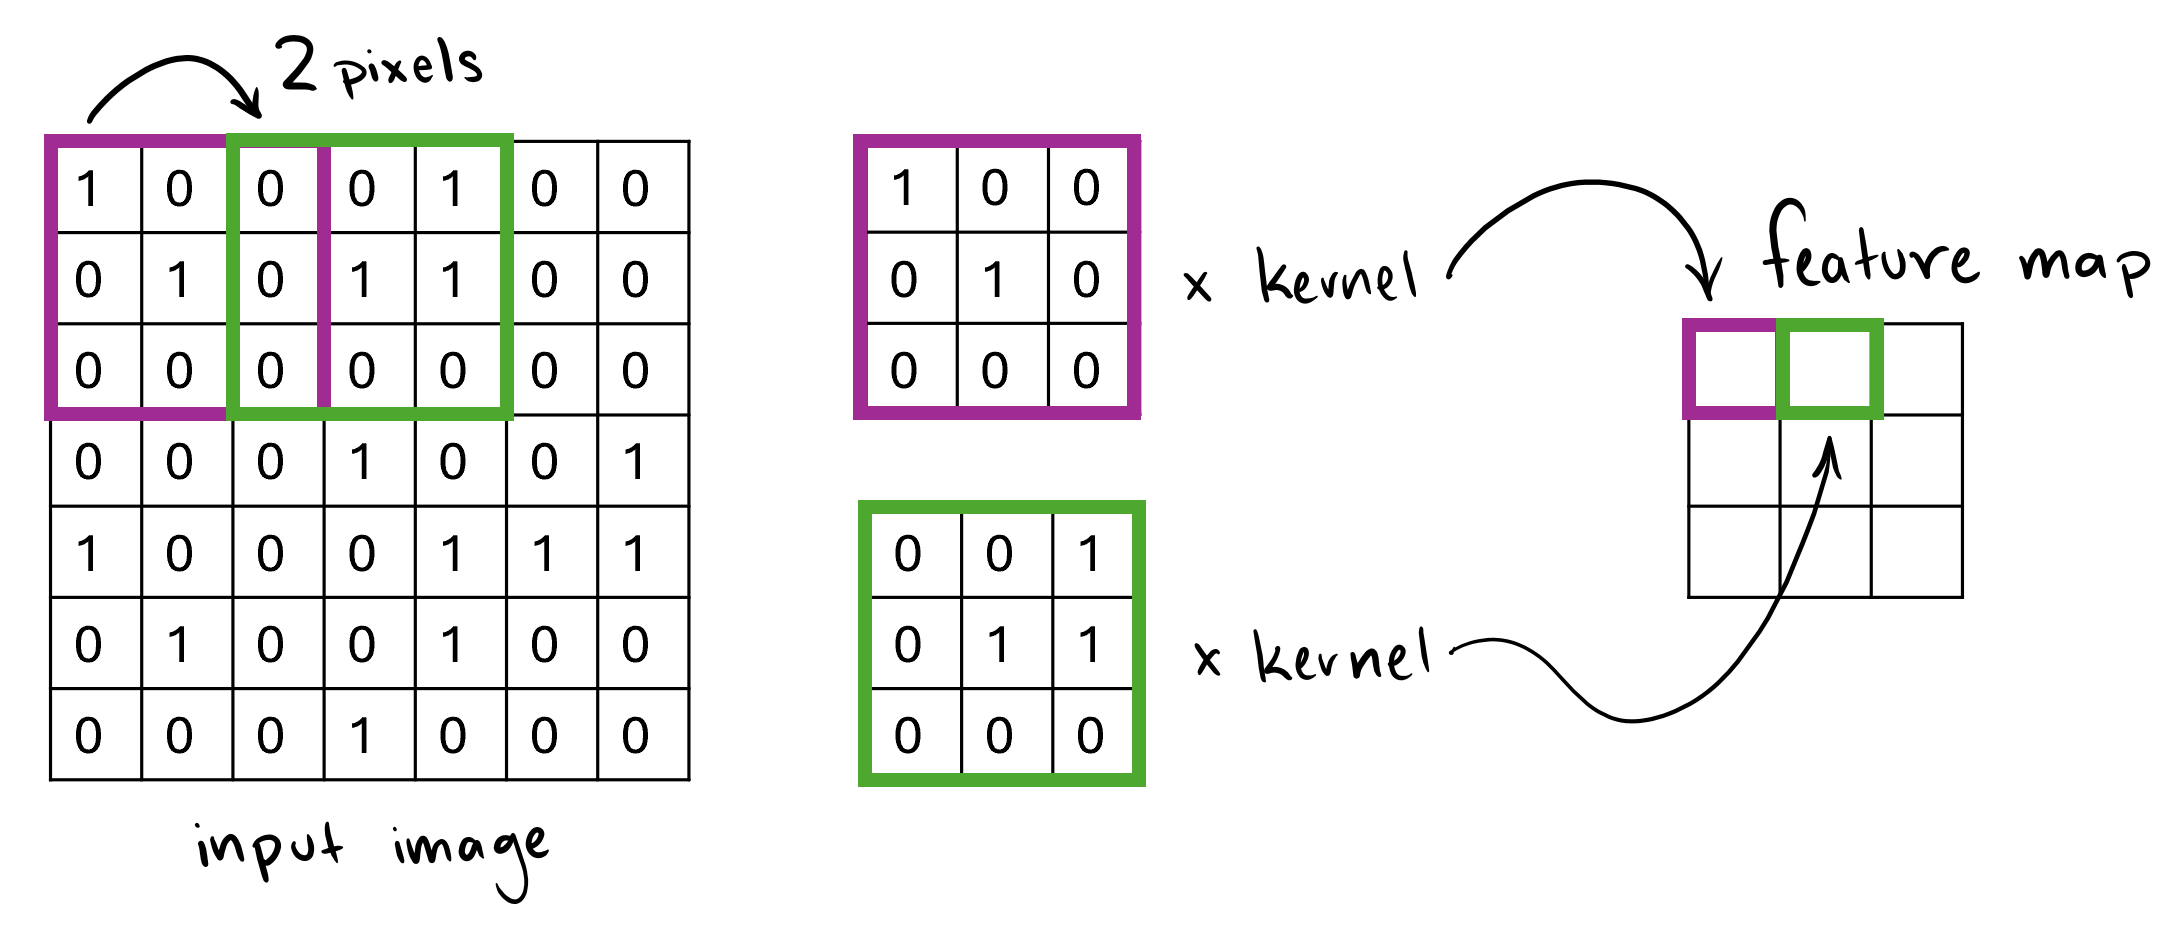
\includegraphics[width=1\linewidth]{cv/stride2eg.png}
            \caption{Illustration depicting a stride of 2 pixels}
            \label{fig:stride2eg}
        \end{figure}

        Padding, on the other hand, refers to extra pixels around the edges of a kernel. These extra pixels, usually having a value of 0, control the size of the outputted feature map. With padding, we can manipulate the size of the feature map in multiple ways, including leaving the feature map with the same dimensions as the input matrix, while still applying the kernel as a filter.

    \subsection{Nonlinearity in CNNs}
        CNNs, like all neural networks, employ \textbf{nonlinearity} to model the complex patterns in their data that cannot be captured by linear transformations alone. Nonlinearity is vital for neural networks - without it, all their calculations would be the equivalent of a single linear operation. Using non-linear functions break this linearity, enabling the model to approximate complex, non-linear decision boundaries, which is essential for tasks like image recognition, object detection, and natural language processing. In CNNs, this nonlinearity is employed after the application of the kernel and with \textbf{activation functions}. Using non-linearity after convolutional layers aids the network in learning hierarchical features of increasing complexity. Early layers learn simple features like edges and textures, while deeper layers combine these to detect more abstract features such as objects or shapes. \break

        CNNs commonly use the \textbf{Rectified Linear Unit or ReLU} activation function. ReLU, as seen in the formula below, is quick, efficient, and requires little computation power. 
        
        $$ReLU(x) = \mathrm{MAX}(0,x)$$
        
        ReLU leaves all positive values unchanged and changes all negative values to 0. This method prevents certain neurons from activating, making the model more efficient and less prone to overfitting. However, stopping neurons from activating also has disadvantages, such as certain features or neural connections `dying out'. This means some neurons will never learn and advance, since their gradients are reset to 0 using this activation function. \break

        In order to address these disadvantages, models sometimes use \textbf{LeakyReLU}. LeakyReLU uses the formula:

        \[f(x)= 
        \begin{cases}
            x,& \text{if } x > 0\\
            \alpha x, & \text{if } x \leq 0
        \end{cases}
        \]

        where $\alpha$ denotes a small positive constant, usually 0.01. In this activation function, negative values are suppressed instead of reset. So neurons will be able to activate, but their activation will be quieter and negative values will continue to have less effect on the final conclusion.

    \subsection{Pooling Layer}
        \large Now, after the convolutional layer, the features in the image are amplified and complex calculations have been used to manipulate the image to extract details from it. Once those calculations are complete, another layer manipulates the image further, summarizing all these little details brought out by the convolutional layer. This is called the \textbf{pooling layer}. The pooling layer simplifies the feature map outputted by the convolutional layer, while retaining the significant features. This reduces the amount of parameters that move on to the next layer and the amount of computation necessary, making the model more efficient. Any further operations done by the model will be done on the `pooled' matrix, with features summarized and simplified through the use of a 2-dimensional filter. For a feature map having dimensions $h \times w \times c$, the dimensions of the map after pooling would be 
        $$\biggl( \frac{h - f + 1}{s} \times \frac{w - f + 1}{s} \times c \biggr)$$
        Note that $f$ is the size of the filter used and $s$ denotes the length of the stride used. \newline

        A common technique used for the pooling layer is \textbf{max pooling}. This operation takes the maximum value in a given section of the feature map and selects that number to represent the section in the summarized map, as seen in the figure below. 

        \begin{figure}[H]
            \centering
            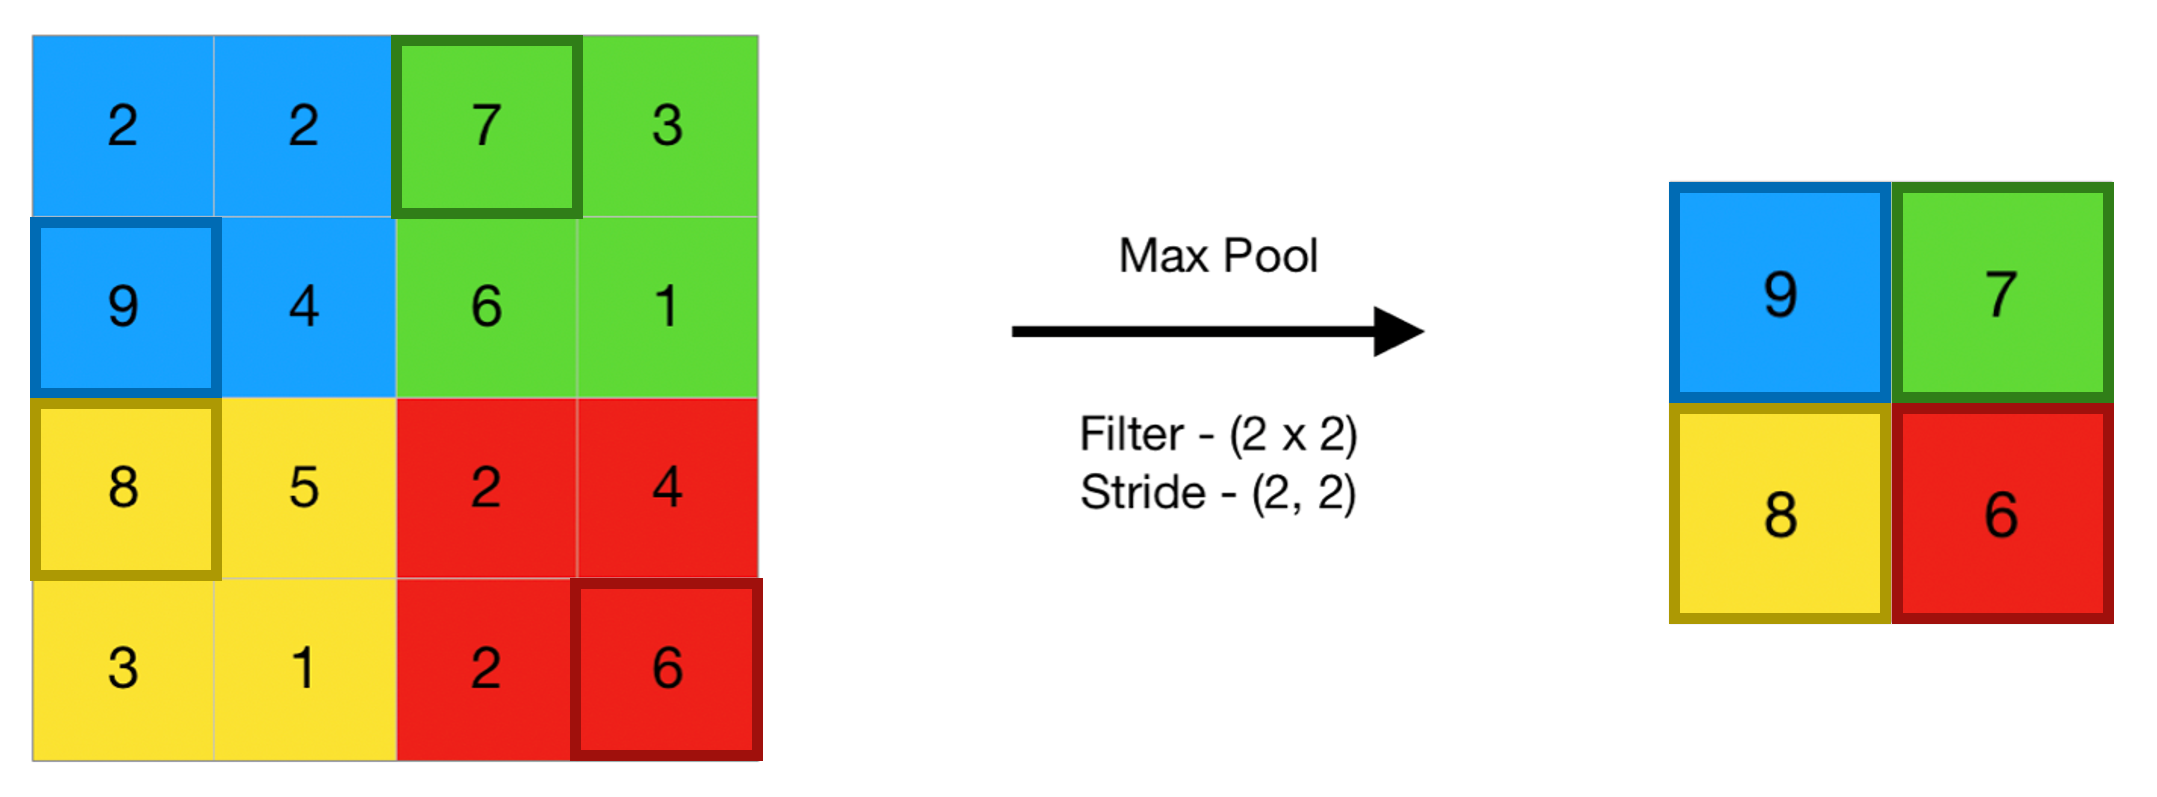
\includegraphics[width=0.75\linewidth]{cv/maxpooling.png}
            \caption{Illustration of the max pooling operation}
            \label{fig:maxpooling}
        \end{figure}

        If we take the section of the map that the max pooling operation is being done on as $Z(i, j)$, we get the following formula for the calculation on $Z(i, j)$. This calculation is done assuming a section size of $2 \times 2$.
        $$Z_{pool}(i, j) = \max \{Z(2i,2j), Z(2i+1,2j), Z(2i,2j+1), Z(2i+1,2j+1)\}$$ 

        \textbf{Average pooling}, another pooling operation, uses a similar methodology. Rather than taking the maximum value however, average pooling chooses the average value of the section rather than the maximum as representation in the pooling matrix. It's $Z_{pool}$ formula for a $2 \times 2$ section is as follows
        $$Z_{pool}(i, j) = \frac{1}{4} (Z(2i,2j) + Z(2i+1,2j) + Z(2i,2j+1) + Z(2i+1,2j+1))$$

        While pooling layers are extremely beneficial in making models more efficient, they have a few disadvantages. As you can see in both the max and average pooling operations, pooling causes significant information loss. Pooling layers minimize the data, meaning we lose information in the process. This loss can cause excess `smoothing' of the image, where finer details are lost.

        \subsection{Fully Connected Layer}
        The \textbf{dense} or \textbf{fully connected layer} is the last layer of a Convolutional Neural Network. Typically, CNNs employ several convolutional and pooling layers before the dense layer, to extract and identify all the necessary features before making a conclusion. Before the input from the last convolutional or pooling layer can be passed to the dense layer, it is flattened into a one-dimensional vector. These dense layers are just neural networks, and, in the cases where the CNN is integrated into another network, they are the neural network processing the features extracted by the CNN. The fully connected layers, or the model in the other case, perform regression or classification operations on the given input to draw a conclusion based on the data. For a single-dimensional input vector $\textbf{x}$, a weight matrix $\textbf{W}$, and a vector of bias terms of each neuron $\textbf{b}$, the formula for the vector of outputs $\textbf{z}$ would be
        $$\textbf{z} = \textbf{W} \cdot \textbf{x} + \textbf{b}$$

        The dense layer also typically uses an activation function when doing a multi-level classification operation. This activation function takes the logits from the previous layer and converts them into probabilities between 0 and 1. The \textbf{softmax activation function}, as seen below, is typically used for this specific operation. 
        
        $$\mathrm{Softmax}(z_i) = \frac{e^{z_i}}{\sum^{n}_{j=1} e^{z_j}}$$
        
        In the formula, $z_i$ denotes the raw logits calculated by the dense layers for class $i$. After applying the softmax operation to raw logits (can hold any numerical value), we get a ``probability distribution'' over all classes. We then select the one with the highest probability, and say that the image given to the CNN belongs to class $i$.

        \subsection{Loss Functions, Optimizers, and Regularization}
        Similarly to neural networks, CNNs also use loss functions, optimizers, and regularization to improve their accuracy. They use many of the same functions that we've covered already, such as \textbf{Cross-Entropy Loss} and \textbf{Mean Squared Error} for loss functions, \textbf{gradient descent} for optimization, and \textbf{dropout} for regularization. \break

        See the figure below for an overview of the entire architecture of a Convolutional Neural Network.  \break
        
        \begin{figure}[H]
            \centering
            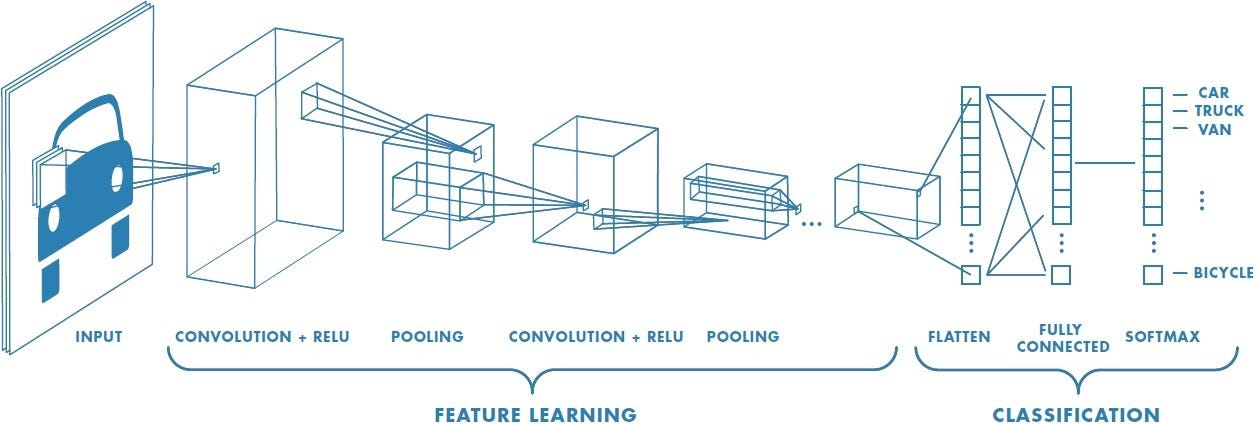
\includegraphics[width=1\linewidth]{cv/full_cnn.png}
            \caption{Illustration of complete architecture of CNN}
            \label{fig:full_cnn}
        \end{figure}
\end{flushleft}

\vspace{10px}
\begin{questionbox}
    \textbf{Synthesis Questions:}
    \begin{enumerate}    
        \item What region of the brain are CNNs (loosely) based off?
        \item Describe, in your own words, what is the purpose of a convolutional layer?
        \item What changes the size of the output feature map, padding or the values populating a kernel?
        \item What changes the values in the output feature map, padding or the values population a kernel?
        \item Why are there usually multiple convolutional and pooling layers in CNNs?
    \end{enumerate}
    \vspace{1px}
\end{questionbox}

\section{Self-Supervised Learning}
\begin{flushleft}
    \large \textbf{Self-supervised learning} or SSL, is a paradigm of machine learning that allows models to learn from useful representations of data. This means that models using SSL don't need large, extensively labeled datasets (datasets that are usually labeled manually), saving time and resources. By employing self-supervised learning, models are able to use unlabeled data to learn. The fundamental idea of self-supervised learning is for the model, when given unlabeled data, to generate labels for said data. These labels will be used as ground truths (like true labels) in further operations. In the first step, the model attempts to identify patterns in the data and then, based on these patterns. assigns labels to the data it feels confident about. Then the model continues its training, using its labels and continuing to learn with backpropagation as normal. The only difference in the training process is that every time the model makes a forward pass, it reassigns the labels to whatever data is it confident about. there are several methods SSL models employ to efficiently and reliably conduct this process.
\end{flushleft}
\subsection{Methods of SSL}
\begin{flushleft}
    \large The first method we will discuss is \textbf{Contrastive Learning}. This is one of the core techniques of self-supervised learning. Contrastive learning works to train the model to distinguish between similar and dissimilar points. Using this training, the model can determine which points should have the same label and which should have different labels. \newline  
    
    To implement contrastive learning, the model typically uses pairs or groups of data points. For example, in image data, the model might be given two views of the same image with slight transformations—like rotations, cropping, or color adjustments—as "positive" pairs. It then receives unrelated images as "negative" pairs. The model is trained to bring the positive pairs closer together in its internal representation space while pushing the negative pairs further apart. \newline 

    Another popular method is called \textbf{predictive tasks}. In this technique, the model is given a scenario in which it must predict the values of some features given the values of other features. For example, it may have to predict missing or hidden sections of images given the rest of the image. Techniques like \textbf{image inpainting} (predicting missing parts of an image) or \textbf{rotation prediction} (learning the correct orientation of rotated images) allow the model to learn contextual and spatial relationships within the image, strengthening its understanding of the data.

    In addition to image inpainting and rotation prediction, predictive tasks can also include techniques such as \textbf{context prediction}, where the model attempts to predict the surrounding context of a specific image region. In this scenario, a portion of the image is masked or hidden, and the model is tasked with inferring the values of the masked area based on the visible context. This process encourages the model to focus on local and global features, enhancing its understanding of how different elements interact within the image. Using predictive tasks, the model will learn more about the data and will be able to label it without supervision.
\end{flushleft}
\subsection{Importance of SSL}
\begin{flushleft}
    \large Self-supervised learning is critical in computer vision because it addresses the challenge of obtaining labeled datasets for image classification. Datasets for computer vision must be extensive and are typically manually labeled, making it much harder to generate the data needed for supervised learning in computer vision tasks. In many fields, such as medical imaging, autonomous driving, and wildlife monitoring, labeled data is scarce or difficult to acquire. Self-supervised learning addresses this issue directly by allowing models to learn directly from unstructured data without the need for extensive labeling. This approach not only reduces the reliance on human labor for labeling but also enhances the model's generalization capabilities across diverse tasks and datasets. Ultimately, self-supervised learning paves the way for more efficient and scalable computer vision solutions, enabling broader applications and improvements in areas like image classification, object detection, and scene analysis.
\end{flushleft}

\vspace{10px}
\begin{questionbox}
    \textbf{Synthesis Questions:}
    \begin{enumerate}    
        \item In your own words, how does self-supervised learning mitigate the shortcomings of supervised learning (think about the training process and data)?
        \item Can you think of any ways in which self-supervised learning is similar to human learning?
        \item What are some specific fields that would benefit from using self-supervised learning for computer vision?
    \end{enumerate}
    \vspace{1px}
\end{questionbox}

\section{Image Segmentation}
\begin{flushleft}
    \large Another method used in computer vision models is \textbf{image segmentation}. This approach focuses on identifying groups of pixels that belong together and works to separate individual objects in images. 
    \begin{figure}[H]
        \centering
        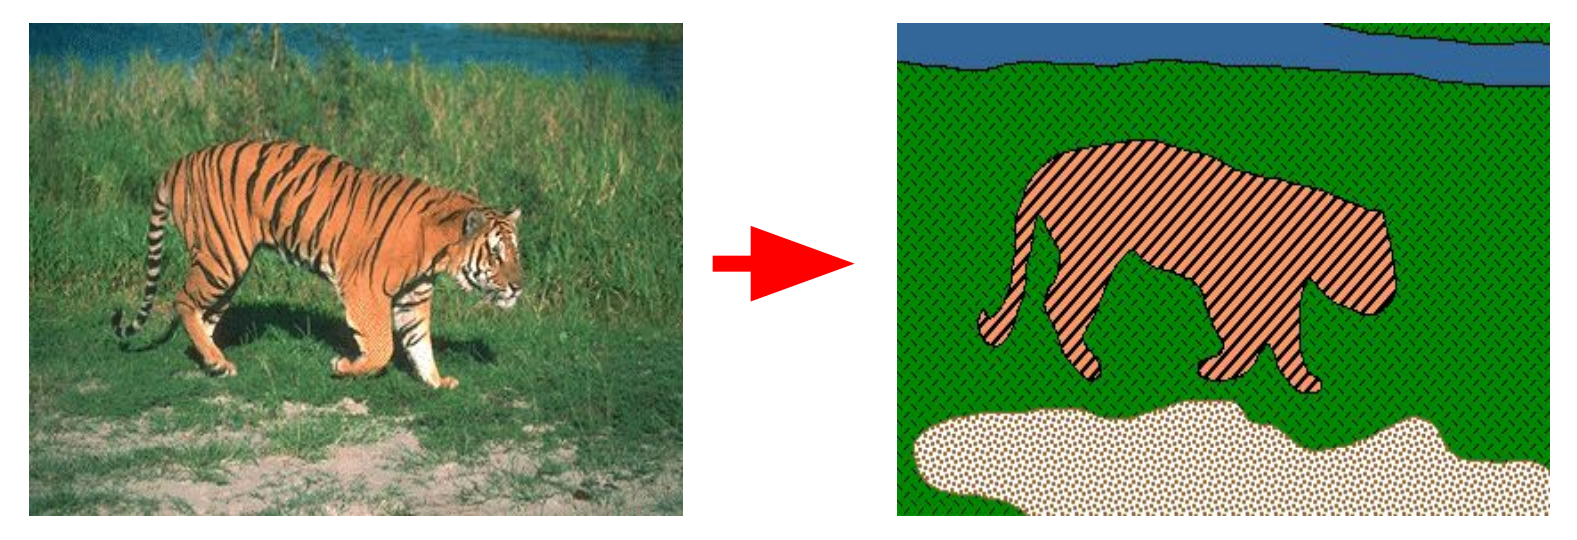
\includegraphics[width=0.75\linewidth]{cv/segmentation-tiger.png}
        \caption{Illustration of high-level image segmentation}
        \label{fig:segmentation-tiger}
    \end{figure}

    By combining individual pixels into groups, image segmentation allows for faster, more efficient image processing. It also allows for more advanced image processing with less computation. Image segmentation is widely utilized in various applications, such as medical imaging, where it assists in identifying tumors or anatomical structures, and in autonomous vehicles, where it helps recognize pedestrians, road signs, and other vehicles. By accurately separating objects from the background, image segmentation enhances the performance of machine learning algorithms and improves decision-making processes. 

    \subsection{Techniques of Segmentation}
    An important concept in image segmentation is \textbf{superpixels}. The term superpixels refers to smaller collections of pixels that are grouped together for a shared characteristic, such as color or texture. The model then is able to treat each superpixel as its own pixel, drastically reducing the amount of data taken in by the model. This reduction in the number of segments that need to be processed leads to more efficient algorithms. \newline

    Superpixels are grouped in several ways. Superpixels are designed to maintain the spatial distance and positioning of their pixels. Therefore spatial coherence is a key factor in the creation of superpixels, meaning that adjacent pixels are more likely to be included in the same superpixel. Additionally, superpixels can be formed through same-color grouping, where pixels with similar color values are clustered together, allowing for the identification of regions that share visual characteristics. Another approach is the grouping of pixels with the same texture, which focuses on the texture features of pixels, clustering them based on patterns and variations in surface properties. These different grouping methods enhance the ability of superpixels to capture meaningful segments of an image, facilitating more efficient and accurate image analysis. \newline

    Segmentation is also used to identify separate entities in images, entities that are larger than a few pixels. There are two main entity classes in segmentation, \textbf{things} and \textbf{stuffs}. Things are objects in images - people, structures, animals, etc. Things have characteristic shapes and have relatively little variance in size. Stuff, on the other hand, refers to classes with amorphic shapes, entities that are fluid and have no characteristic shapes. Sky, water, grass, and other backgrounds are typical examples of stuff. Stuff also doesn't have countable, individual instances, like things two. A blade of grass and a field of grass are both grass, but a bear and fives bears are not both a bear. There are some entities that, under certain image conditions, can be both things or stuff. For example, a large group of people can be interpreted as multiple ``persons” — each a distinctly shaped, countable thing — or a singular, amorphously shaped ``crowd”. \break

    The simplest method of entity segmentation is \textbf{semantic segmentation}. This method assigns a semantic class to each pixel, but does not identify classes or differentiate between thing and stuff classes. Semantic segmentation focuses on drawing boundaries between objects but does not assign labels to them or identify different instances of the same object. Other more complex methods of segmentation are \textbf{instance segmentation} and \textbf{panoptic segmentation}. To learn more about segmentation, see \href{https://tinyurl.com/7kz8dkhu}{IBM Image Segmentation}.
\end{flushleft}

\vspace{10px}
\begin{questionbox}
    \textbf{Synthesis Questions:}
    \begin{enumerate}    
        \item How do superpixels enhance the efficiency of image segmentation algorithms?
        \item In what scenarios might an entity be classified as both a ``thing" and ``stuff" in image segmentation? How might this dual classification impact the effectiveness of semantic segmentation methods?
    \end{enumerate}
    \vspace{1px}
\end{questionbox}

\section{When to Use Computer Vision}
\begin{flushleft}
    \large Computer vision is a field with a long history and many decades of research put into it. People have been working on these problems long before the recent waves of deep learning and machine learning. As such, it is worth digging deep into CV literature to find the best and most efficient model or architecture for your specific task. Some tools created with computer vision in mind (i.e. CNNs) can also be used in non-CV tasks if you want to leverage spatial information within your data.
\end{flushleft}

\section{Conclusion (CV)}
\begin{flushleft}
    \large 
    This section covered some of the fundamental concepts within computer vision. By leveraging techniques like Convolutional Neural Networks (CNNs) and self-supervised learning, we’ve learned how machines can mimic human vision, identifying objects, segmenting images, and even understanding complex scenes. This is no small feat; it means computers can learn to see and interpret visual information, making them more intuitive and responsive to our needs. This deep dive reveals just how crucial CV is for making sense of the visual world around us in the modern era. Computer vision serves as a bridge between the raw data captured by cameras and the meaningful insights we derive from those images. It plays a vital role in our increasingly digital lives, impacting everything from social media filters to advanced security systems.  \break
    
    Understanding these methods is key because they enable computers to perform tasks that once seemed out of reach, like accurately detecting tumors in medical imaging or helping autonomous vehicles navigate safely. For instance, in healthcare, CNNs can analyze scans and X-rays, significantly reducing the time it takes to identify critical conditions, ultimately leading to faster diagnoses and better patient outcomes. Similarly, in the realm of autonomous driving, computer vision allows vehicles to recognize pedestrians, road signs, and obstacles in real-time, enhancing safety and efficiency on the roads. These advancements not only improve operational capabilities but also build trust in technology that plays such a significant role in our lives.
\end{flushleft}


\section*{REINFORCEMENT LEARNING}
\addcontentsline{toc}{section}{\protect\numberline{}REINFORCEMENT LEARNING}
\section{What is Reinforcement Learning?}
\subsection{Problem Definition}
\begin{flushleft}
    \large Reinforcement Learning is a subfield of AI that concerns itself with optimizing behavior of \textbf{agents} in \textbf{environments} using \textbf{rewards}. It is focused on finding efficient ways to train an agent (think of Mario) to reach a goal (the flag) within an environment (World 1-1) by offering rewards (coins, distance to flag, etc.). The example of Mario is actually quite narrow, as it restricts RL to ``game-like'' situations only. Although many popular examples of RL are about solving/beating some puzzle/game, the true extent of the field is much richer. There are projects that heavily rely on concepts from RL that may not be obvious at first. For example, AlphaTensor is a model published by Google DeepMind that searches for ways to perform large matrix multiplications in fewer operations than the standard method that we see commonly used. A significant part of this algorithm is considered reinforcement learning. Also, many Large Language Models (LLMs) use reinforcement learning with human feedback (RLHF) for finishing touches in their training process. ChatGPT is one of these LLMS! Neither of these examples present as a game or puzzle, yet RL is used extensively within them. \break
    
    As mentioned before: many examples of RL \textit{are} within game-like environments, but it is important to understand that the ``agent'' and ``environment'' can be almost anything that you wish to define them as (there are a few restrictions). A more general definition of RL can perhaps be \textit{``using trial and error to learn a strategy that maximizes reward in a selected environment''}. The field of reinforcement learning pulls a lot from optimal control theory, machine learning, probability theory, and a little bit of psychology and neuroscience. Stepping through all of RL in an article is nearly impossible, there are whole books on $\frac{1}{100}$ of this content. As such, this article will introduce common symbols, provide some priming on large RL subcategories, and end with a couple algorithms and their strengths/weaknesses.
\end{flushleft}

\subsection{Common Symbols and Definitions}
\begin{flushleft}
    \large Here are some common symbols used in RL and their meanings. Analogies have been provided for ease of understanding.\break

    \textbf{State}: $s \in \mathcal{S}$
    \begin{itemize}
        \item Most commonly represented as a vector, a state is a snapshot of the world at some timestep $t$ (often denoted as $s_t$). A state records important information about the current frozen moment in time that often determines what will happen next. The way the vectors represent the state is a choice dependent on the problem.
        \item An example of a state from the game Pong would be a vector holding the y-positions of the paddles, the velocity of the paddles, the position of the ball, and the velocity of the ball. It could also contain the score. Note that just raw positions are not ``good enough'' to comprise a state, because it would be difficult to determine what could happen next from just positions (i.e. The ball is at (0,0). Is it moving left or right?)
    \end{itemize}

    \textbf{Action}: $a \in \mathcal{A}$
    \begin{itemize}
        \item An action is a choice that the agent (see below) makes within the environment that often influences the subsequent state. Actions are taken at a time $t$ and are denoted as $a_t$. Actions can be represented as scalars between a range (0-1), a one-hot encoded vector ([1,0,0,0]), or an unbounded vector ([0.5, -3, 2, 0.001]). The choice of how an action is represented depends on the problem.
        \item An example of an action from the game Pong would be a number between -1 and 1 determining the speed of vertical movement for the next timestep. Note that this implicitly encodes the ``do nothing action'' of 0 (standing still).
    \end{itemize}

    \textbf{Agent}:
    \begin{itemize}
        \item An agent is an actor that takes in the current state of the environment and acts optimally (or tries to) in order to maximize reward. 
        \item An example of an agent would be Mario, the character.
    \end{itemize}

    \textbf{Policy:} $\pi$
    \begin{itemize}
        \item A policy is a function that outputs action(s) given the state of the environment. Agents and policies are closely tied together because the \textit{job of an agent is to learn a good policy}. There are two main types of policies. \textbf{Deterministic policies} are represented as $\pi(s) \rightarrow a$, meaning that there is a mapping between each state of the world and the best action to take at that time. A \textbf{stochastic policy} can be defined as $\pi(a_t|s_t)$. This means that given a state at time $t$, a policy will give you a distribution over all possible actions, with probabilities corresponding to how good that action is at that timestep. The agent can then select an action based on these probabilities.
        \item An example of a policy would be \textit{how Mario behaves} based on his surroundings. Note the difference between this and the character Mario. It is similar to the difference between policy and agent.
    \end{itemize}

    \textbf{Environment}:
    \begin{itemize}
        \item A space, the world, that the agent can interact with and influence. Can be thought of as ``all possible states''. Also implicitly contains \textbf{transition dynamics}, or probability distributions of future states depending on the current state and action ($p(s_{t+1}|s_t,a_t)$)
        \item An example of an environment would be World 1-1 from Mario. Not just a snapshot of the world at a time $t$, but the idea of this ``level'' to beat. Transition dynamics for this environment would be the physics engine and enemy movement.
    \end{itemize}

    \textbf{Reward}: $r$
    \begin{itemize}
        \item Perhaps one of the most important terms. A reward is a scalar value given to the agent after it takes an action, determined through a \textbf{reward function} that considers the state-action pair at time $t$ and its ``optimality''. This is represented as $R(s_t, a_t) = r_t$. Generally, the higher $r$ is, the better the action $a_t$ the agent took based on state $s_t$. This reward value serves as a learning signal for the agent, and is used to update its parameters to improve performance on future actions.
        \item For example, if Mario is standing next to lava (state $s_t$) and he took the action ``go forward'', the reward $r_t$ as determined by $r(s_t, a_t)$ would be very low, perhaps even negative. Mario dies, and the agent tries again. Once this same lava pit is reached, Mario instead takes the ``jump'' action and lands on the other side of the lava pit safely. Since he moved closer to his goal, the reward function spits out a high reward. This reinforces the rule ``If next to lava, then jump''. \textit{Through this trial and error, the policy is slowly updated until Mario is able to maximize reward by beating the level!}
    \end{itemize}

    \textbf{Trajectory}: $\tau$
    \begin{itemize}
        \item A compact way to represent the path an agent took through the environment during one \textbf{episode} and the rewards it received for doing so. An episode begins with the very first state $s_0$ and continues until the agent dies, reaches its goal, or runs out of time. Trajectories are useful because they store enough information to ``replay'' the episode entirely. For an episode of length $T$, the trajectory would be $\tau = (s_0, a_0, r_0, s_1, a_1, r_1,...,s_T, a_T, r_T)$.
        \item A trajectory in Mario would record every frame of the game, every action taken at each timestep, and the rewards given to Mario. You can think of it as ``recording'' an agent's playthrough of World 1-1.
    \end{itemize}
    
\end{flushleft}

\subsection{Markov Decision Process}
\begin{flushleft}
    \large I mentioned earlier that there were a few restrictions to defining something as an RL problem. The \textbf{Markovian property} is one of them. The transitions within an environment from state to state must be a Markovian decision process (MDP). For a decision process to be Markovian, the transition from state $s_t$ to $s_{t+1}$ should be independent of the ``history'' of that state, i.e. states $s_0, s_1,...,s_{t-1}$. Why is this helpful? Well firstly, it makes it such that a policy can be learned \textit{much} easier since we have less unique state-action pairs to deal with. \break
    
    Think about it: If there were 100 states and 4 actions, a policy would only need to deal with $100 \times 4$ state-action pairs \textit{total} if the transition dynamics were Markovian. With today's compute, you can even create a table that maps each state to the optimal action for that state and do it with brute force search. However, if a state's history needs to be considered, then determining the proper action to take at $s_t$ would require considering the $100^t$ paths possible to reach $s_t$. With the decision process not being Markovian, Mario jumping up over a block and ending up past it, and Mario running under it but ending up at the \textit{same spot} would \textit{not} be the same state $s_t$! This combinatorial explosion makes things way harder. \break

    Another way to formalize this can be seen below:

    $$p(s_1, s_2, s_3,...,s_t) = p(s_1)p(s_2|s_1)p(s_3|s_2)...p(s_t|s_{t-1})$$

    The left-hand side of the equation is the probability of events $s_1$ AND $s_2$ AND $s_3$... happening. Now on the right hand side; Note how $p(s_3|s_2)$ (probability of $s_3$ happening given that $s_2$ has already happened) does not include $s_1$ anywhere, despite it being in the ``history'' of $s_2$. The movement between $s_2 \rightarrow s_3$ is independent of $s_1$. With an MDP, you can find the probability of a sequence of states quite easily with much less compute than if you had to consider the history of the state. This algorithm tries to get an RL agent to accomplish a task by learning from an expert doing the same task.  \break

    This is very important: how you define states is often what makes a problem behave as an MDP. Remember the example about Pong states earlier? If we were to capture \textit{only the positions} of the paddles/ball, then we would NOT have an MDP. This is because by looking at the ball at a position (e.g. (0,0) at $t=1$) we cannot tell if it is moving forward, backward, up, or down. We would need to look into its history to determine that. If the ball was at (-1,-1) at $t=0$, and now is at (0,0), we can assume that it has a velocity of [1,1] and will be at (1,1) at $t=2$. Since the transition from $s_1 \rightarrow s_2$ is dependent on $s_0$, this is not an MDP. However, if we include the velocity $[1,1]$, into the state along with the position, this problem goes away! We no longer need to look into a state's history to determine how it will transition. Everything is captured in this clever definition of a state.
    \end{flushleft}

\subsection{On vs. Off-Policy RL}
\begin{flushleft}
    \large A short but important note on the terms \textbf{on-policy} and \textbf{off-policy} RL. If you decide to pursue RL on a deeper level, the distinction will become more important as the math behind algorithms in each has different assumptions and conclusions. However, for simplicity, here are some basic definitions: \break

    \textbf{On-Policy}: On-policy reinforcement learning algorithms can only use information from the \textit{current trajectory} to update its policy. In other words, the agent tries to solve the problem (perhaps a few times), updates its policy based on the rewards received, and tries again. Once the policy is updated, the information (trajectories) gathered using the pre-update policy becomes ``useless''. Since the agent is following a fresh new policy, it is mathematically improper to draw examples from a different distribution to update itself. While algorithms that are on-policy tend to be more stable, they are much less \textbf{sample efficient} and have high variance. \break
    
    \textit{Quick Definition:} Sample efficiency is how well a model can use the information provided within datapoints to learn patterns. A sample efficient model would just need to see 10 examples to learn a pattern. A non-sample efficient model may need 1000's. Your brain is one of the most sample efficient models out there! \break

    \textbf{Off-Policy}: Off-policy algorithms are allowed to use information collected from ``older'' policies to update the current one. This makes them much more sample efficient, as you can use the same trajectory to optimize the policy many times as opposed to just once. Off-policy RL algorithms, while more sample efficient, tend to be less stable and require a few tricks to work properly.
\end{flushleft}

\begin{questionbox}
\textbf{Synthesis Questions:}
\begin{enumerate}
    \item Think of a video game, board game, or puzzle that you like. Then do the following:
    \begin{itemize}
        \item Define the environment, and agent. What is the positive reward that the agent should chase? Try to tie this to a mathematically calculable formula (i.e. $r = \frac{1}{d}$ where $d$ is the distance to the flagpole).
        \item Define as concretely as possible a representation of states and actions for this environment/agent. Can you show that the states you chose could form an MDP?
    \end{itemize}
    \item Do you think an on-policy or off-policy algorithm would suit your problem better (there is no right answer for this one, it is a hard question)?
\end{enumerate}
\end{questionbox}


\section{Imitation Learning}
\subsection{Basic Behavior Cloning}
\begin{flushleft}
    \large Taking a step back from the plethora of notation, we will approach RL somewhat naively through \textbf{behavior cloning}, one of the simplest forms of RL. Rewards are not even needed in this problem formulation, and it blurs the lines between supervised learning and reinforcement learning. \break

    In this problem formulation, we assume we have an expert from which we get many $(s^{*}, a^{*})$ pairs. The superscript stars denote that this information is ``optimal''. We assume that the expert has solved the problem perfectly. For example, we would allow a human with a remote control to operate a robotic arm and perform a task. The telemetry data would be recorded and this dataset is referred to as $\mathcal{D}$, from which we can sample $(s^{*}, a^{*})$ pairs. We can now write an optimization objective:

    $$\underset{\theta}{\textrm{argmax}}\biggl[\mathbb{E}_{(s^{*},a^{*}) \sim \mathcal{D}}[\mathrm{log}\pi_\theta(a^{*}|s^{*})]\biggr]$$

    This seems complicated so let's break it down:

    $$\downarrow$$
    $$\underset{\theta}{\textrm{argmax}}\biggl[ \cdot \biggr]$$

    Argmax with an underset $\theta$ means that we wish to find some $\theta$ that will result in the maximum possible value for the function that follows. For example:

    $$\underset{x}{\textrm{argmax}}\biggl[-x^2\biggr] = 0$$

    0 is the value of $x$ that maximizes $-x^2$, so $\underset{x}{\textrm{argmax}}$ = 0.
    
    $$\mathbb{E}_{(s^{*},a^{*}) \sim \mathcal{D}}[\cdot]$$
    $$\downarrow$$
    $$\underset{\theta}{\textrm{argmax}}\biggl[ \mathbb{E}_{(s^{*},a^{*}) \sim \mathcal{D}}[\cdot] \biggr]$$

   A subscript of an expectation can be somewhat ambiguous, and mean slightly different things depending on context. In this case, we are defining where $s^{*}$ and $a^{*}$ come from (the expert distribution $\mathcal{D}$). This becomes important because these two variables are part of the final term we introduce:

   $$\mathrm{log}\pi_\theta(a^{*}|s^{*})$$
   $$\downarrow$$
   $$\underset{\theta}{\textrm{argmax}}\biggl[\mathbb{E}_{(s^{*},a^{*}) \sim \mathcal{D}}[\mathrm{log}\pi_\theta(a^{*}|s^{*})]\biggr]$$

   $\pi_\theta$ is the policy, parameterized by $\theta$. What this means is that if this policy is represented by a neural network, \textit{then $\theta$ are the weights and biases}. $\mathrm{log}\pi_\theta(a^{*}|s^{*})$ is the ``log-probability'' of the model choosing $a^{*}$ given $s^{*}$. The highest this probability can be is 1. Note that the logarithm of 1 evaluates to 0. Anything below 1 will evaluate to be exponentially more negative/worse. So if we wish to find the weights and biases ($\theta$) that maximize $\mathrm{log}\pi_\theta(a^{*}|s^{*})$, we need to select weights and biases that assign a probability of 1 to $a^{*}$ given $s^{*}$ and 0 to all other actions. We know that $a^{*}$ and $s^{*}$ come from an expert distribution $\mathcal{D}$ thanks to the subscript. Therefore if we find $\theta$, we have a policy that will act optimally given the states it has seen! This notation may seem heavy, but it is a primer for more complex algorithms. \break

   How this is implemented in code is quite simple. We simply take every $(s^{*},a^{*}) \sim \mathcal{D}$ pair and label the $s^{*}$ as the data and the $a^{*}$ as the label. We then train a neural network on this data (input dimensionality is the dimensionality of $s$, output dimensionality is the dimensionality of $a$), and call it $\pi_\theta$. We now have a policy that can accept a state, and act accordingly. This all seems much too simple though. What is the drawback?
\end{flushleft}

\subsection{Problems with Behavior Cloning}
\begin{flushleft}
    \large There are two compounding problems with behavior cloning that make a basic implementation mostly unviable for complex situations. \break
    
    The first is that it has \textbf{quadratically compounding error}. There is a proof for this, but it is also intuitive. Say, due to physical forces or minor perturbations, that a robot cloning the behavior of a human gets 0.1cm off from where it should be after taking action $a_t^{*}$ at $s_t$ (optimal action at state $s_t)$. We are now in dangerous territory, as the state the robot is in currently is not found in any training example. As a result, the robot takes a sub-optimal action and ends up 1cm off track. It will be near impossible for the robot to complete its task after a few more missteps, and now it is grabbing your ear instead of the apple it was supposed to. Behavior cloning leads to \textit{very precarious paths to follow}. If the robot can stay perfectly on track and nothing new comes up, then it is able to complete the task perfectly. This is not really useful though. You may as well resort to optimal control theory for robotics, which give you much more guarantees and a little more flexibility. One way to mitigate this is to add lots of training examples, but to even begin to the solve the problem, you need an exorbitant amount of data. There are more intelligent ways to do this, like the DAgger algorithm discussed later. \break

    The second problem is called \textbf{mode averaging}. If we have two paths around an obstacle, for example a tree, we can go around it to the left or to the right. A human knows there is no inherent difference between these two paths, and takes each one with equal probability. However, training a model on this data does not mean the model will also go around the tree in these two ways. Instead it \textit{averages} the two behaviors and ends up going straight into the tree. It is clear that this is sub-optimal behavior, but it is an unavoidable consequence if you have a policy with one mode. For example, a Gaussian policy has only one peak, and will pick one ``best'' action, which will be in between the two peaks of the expert distribution, and this means crashing. One way to mitigate this is to choose a more expressive policy class. A mixture of Gaussians, for example, can have $\geq$ 1 peak. This prevents the mode averaging problem but increases the complexity of your model by a lot.

    \begin{figure}[H]
        \centering
        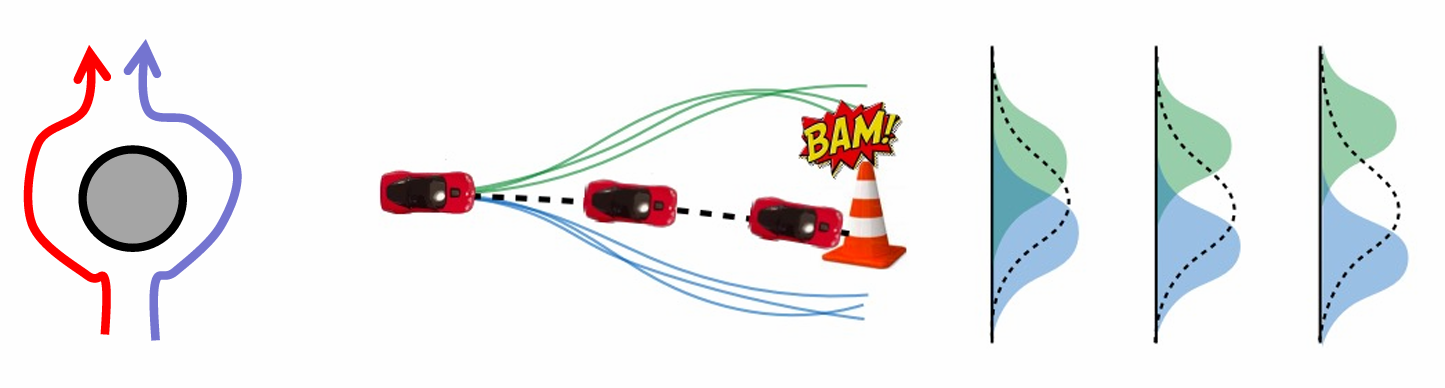
\includegraphics[width=0.9\linewidth]{rl/modeavg.png}
        \caption{An illustration demonstrating the issues that arise from mode-averaging within behavior cloning algorithms. The green and blue peaks represent choosing to go left or right around the obstacle, and the black dashed line represents what a simple policy will converge on.}
        \label{fig:modeavg}
    \end{figure}
\end{flushleft}

\section{Proofs for Problems with Behavior Cloning}
% \subsection{Quadratically Compounding Error}
% \begin{flushleft}
%     \large Below is a walkthrough demonstrating how basic behavior cloning has quadratically compounding error: \break

%     To analyze the effects of deviation from the expert, we create a cost function that gives us 1 when the agent deviates from the expert and 0 otherwise. This will let us quantify the number of deviations from the expert throughout an episode. $a^{*}$ represents the action the expert policy ($\pi_e$) would take at time $t$: $a^{*} = \pi_e(s_t)$.

%     $$c(s_t, a_t) = \begin{cases} 
%           0, & \textrm{if } a_t = a^{*} \\
%           1, & \textrm{otherwise} 
%        \end{cases}
%     $$

%     We also assume the ``worst case scenario'', meaning that once the agent takes a decision that takes it off of the path of the expert, we have no guarantees that it will ever find its way back on track and penalize it heavily. The earlier it goes off track, the higher the penalty. A mistake at time $t = 0$ will incur a penalty of 1 for each subsequent timestep until the episode ends. We say that an episode has length $H$. So:

%     \begin{itemize}
%         \item If $a_t \neq a^{*}$  when $t=0$ $\rightarrow$ Cost = $H$
%         \item If $a_t \neq a^{*}$  when $t=1$ $\rightarrow$ Cost = $H-1$
%         \item If $a_t \neq a^{*}$  when $t=2$ $\rightarrow$ Cost = $H-2$
%         \item ...
%         \item If $a_t \neq a^{*}$  when $t=H-1$ $\rightarrow$ Cost = $1$
%         \item If $a_t \neq a^{*}$  when $t=H$ $\rightarrow$ Cost = $0$
%     \end{itemize}

%     We can write this in summation form as:

%     $$\sum_{t=0}^H \biggl[ \sum^{H-t} c(s_t, a_t)\biggr]$$

%     Because we know that $\pi_\theta$ is somewhat imperfect, we assign a probability $\epsilon$ which represents the chance that the agent picks an action different from the expert:

%     $$p(\pi_\theta(s_t) \neq a^{*}) = \epsilon$$

%     We finally take the expected value of the cost throughout an episode and bound it. We assume that $s_t$ and $a_t$ come from $\pi_\theta$:

%     $$\mathrm{Expected\;Cost} = \mathbb{E}\sum_{t=0}^H \biggl[ \sum^{H-t} c(s_t, a_t)\biggr]$$

%     We can use Linearity of Expectation (LOE) to move the expectation inside the summations:

%     $$\mathrm{Expected\;Cost} = \sum_{t=0}^H \biggl[ \sum^{H-t} \mathbb{E}[c(s_t, a_t)]\biggr]$$

%     The expected value of an indicator variable (in this case $c(s_t,a_t)$) is equal to the probability of that event ocurring. We said earlier that the probability the agent chooses an action different from the expert is $\epsilon$:

%     $$\mathrm{Expected\;Cost} = \sum_{t=0}^H \sum^{H-t} \epsilon$$

%     We can now create a quadratic upper bound:

%     \begin{align*}
%         \mathrm{Expected\;Cost} &= \sum_{t=0}^H \sum^{H-t} \epsilon \\
%         &= H\epsilon + (H-1)\epsilon + (H-2)\epsilon +...+ \epsilon + 0\\
%         &\leq H\epsilon + H\epsilon + H\epsilon +...+ H\epsilon\\
%         \mathrm{Expected\;Cost} &\leq H^2\epsilon
%     \end{align*}

%     Now we can clearly see that the expected error over an episode with length $H$ can be quadratically compounding.
% \end{flushleft}

\subsection{Mode Averaging}
\begin{flushleft}
    \large Below is a walkthrough demonstrating how mode-averaging comes out as a problem in behavior cloning: \break

    Take our original behavior cloning objective

    $$\underset{\theta}{\textrm{argmax}}\biggl[\mathbb{E}_{(s^{*},a^{*}) \sim \mathcal{D}}[\mathrm{log}\pi_\theta(a^{*}|s^{*})]\biggr]$$

    We define $\pi_e$ as the expert policy. Under the expectation $\mathbb{E}_{(s^{*},a^{*}) \sim \mathcal{D}}$, $\mathrm{log}\pi_e(a^{*}|s^{*}) = 0$ is always true. This is because the expert policy will always assign $a^{*}$ (optimal action) a probability of 1 given a state $s^{*}$. $\pi_e(a^{*}|s^{*}) = 1$, $\mathrm{log}(1) = 0$, so  $\mathrm{log}\pi_e(a^{*}|s^{*}) = 0$. We can therefore insert into the equation:

    $$\underset{\theta}{\textrm{argmax}}\biggl[\mathbb{E}_{(s^{*},a^{*}) \sim \mathcal{D}}[\mathrm{log}\pi_\theta(a^{*}|s^{*}) - \mathrm{log}\pi_e(a^{*}|s^{*})]\biggr]$$

    Split the expectation into two nested expectations. $(s^{*},a^{*}) \sim \mathcal{D}$ can be rewritten as $s^{*} \sim p_{\pi_e}(\cdot)$ followed by $a^{*} \sim \pi_e(\cdot|s^{*})$. In english, this means we get a state $s^{*}$ by sampling from possible states the expert ($\pi_e$) has explored and then sample the action $a^{*}$ from the policy $\pi_e$ given that it considers $s^{*}$. The end result is the same, as we have the variables $s^{*}$ and $a^{*}$ to use, and they come from the expert.

    $$\underset{\theta}{\textrm{argmax}}\biggl[\mathbb{E}_{s^{*} \sim p_{\pi_e}(\cdot)}[\mathbb{E}_{a^{*} \sim \pi_e(\cdot|s^{*})}[\mathrm{log}\pi_\theta(a^{*}|s^{*}) - \mathrm{log}\pi_e(a^{*}|s^{*})]]\biggr]$$

    Invert the whole expression from an argmax to an argmin by multiplying by -1, which carries through all the expectations because $a\mathbb{E}[X] = \mathbb{E}[aX]$.

    $$\underset{\theta}{\textrm{argmin}}\biggl[\mathbb{E}_{s^{*} \sim p_{\pi_e}(\cdot)}[\mathbb{E}_{a^{*} \sim \pi_e(\cdot|s^{*})}[\mathrm{log}\pi_e(a^{*}|s^{*}) - \mathrm{log}\pi_\theta(a^{*}|s^{*})]]\biggr]$$

    Use properties of logarithms to rewrite the innermost term:

    $$\underset{\theta}{\textrm{argmin}}\biggl[\mathbb{E}_{s^{*} \sim p_{\pi_e}(\cdot)}[\mathbb{E}_{a^{*} \sim \pi_e(\cdot|s^{*})}[\mathrm{log}\frac{\pi_e(a^{*}|s^{*})}{\pi_\theta(a^{*}|s^{*})}]]\biggr]$$

    For the final step, we must introduce the concept of F-divergence. An F-divergence is, in simple terms, a function that measures the ``distance'' between two functions. The general form of an F-divergence $D_f$ is:

    $$D_f(p(x),q(x)) = \mathbb{E}_{q(x)} \biggl[ f\biggl( \frac{p(x)}{q(x)}\biggr)\biggr]$$
    
    You may be familiar with Kullback-Leibler Divergence (KL divergence) which is a form of F-divergence. KL divergence quantifies the difference between two probability distributions. If you define an F-divergence with $f(x) = x\mathrm{log}(x)$, you get what is called the \textbf{forward KL divergence}.
    
    $$\mathrm{Forward\;KL\;Divergence} = D_{KL}(p(x),q(x)) = \mathbb{E}_{p(x)} \biggl[\mathrm{log}\frac{p(x)}{q(x)}\biggr]$$
    
    A quick proof of this fact is shown below. We use the property that $\mathbb{E}_{q(x)}[p(x)] = \int p(x)q(x)\;dx$.

    \begin{align*}
        \textrm{Given: }f(x) \leftarrow x\mathrm{log}x \\
        D_f(p(x),q(x))\ &= \mathbb{E}_{q(x)} \biggl[ \frac{p(x)}{q(x)}\mathrm{log}\frac{p(x)}{q(x)}\biggr]\\
        &= \int \frac{p(x)}{q(x)}\mathrm{log}\frac{p(x)}{q(x)}q(x)\;dx\\
        &= \int p(x)\mathrm{log}\frac{p(x)}{q(x)}\;dx\\
        D_{KL}(p(x),q(x)) &= \mathbb{E}_{p(x)} \biggl[\mathrm{log}\frac{p(x)}{q(x)}\biggr]
    \end{align*}

    We can apply the definition of forward KL divergence to the inner expectation shown before.

    $$\mathbb{E}_{a^{*} \sim \pi_e(\cdot|s^{*})}[\mathrm{log}\frac{\pi_e(a^{*}|s^{*})}{\pi_\theta(a^{*}|s^{*})}] = D_{KL}(\pi_e(\cdot|s^{*}),\pi_\theta(\cdot|s^{*}))$$

    We are in this expression calculating the KL divergence between the expert policy action distribution given state $s^{*}$ and the agent's action distribution given state $s^{*}$. We can now insert this back into the original equation and draw some insights:

    $$\underset{\theta}{\textrm{argmax}}\biggl[\mathbb{E}_{(s^{*},a^{*}) \sim \mathcal{D}}[\mathrm{log}\pi_\theta(a^{*}|s^{*})]\biggr] = \underset{\theta}{\textrm{argmin}}\biggl[\mathbb{E}_{s^{*} \sim p_{\pi_e}(\cdot)}[D_{KL}(\pi_e(\cdot|s^{*}),\pi_\theta(\cdot|s^{*}))]\biggr]$$

    We now see the original behavior cloning problem formulation written as an F-divergence (more specifically, KL divergence) minimization problem. \textit{Since the F divergence is forward KL divergence, it is mode-averaging by nature}. In other words, trying to minimize the forward KL divergence between a multimodal expert policy $\pi_e$ and a single-mode actor policy $\pi_\theta$ will result in finding a policy that does not fit to either mode, but seeks to the mean of both. Seeing the KL divergence clearly in the equation makes this an unavoidable fact. This gives us a much more concrete basis for why we should expect to observe the crashing behavior discussed earlier!

    \begin{figure}[H]
        \centering
        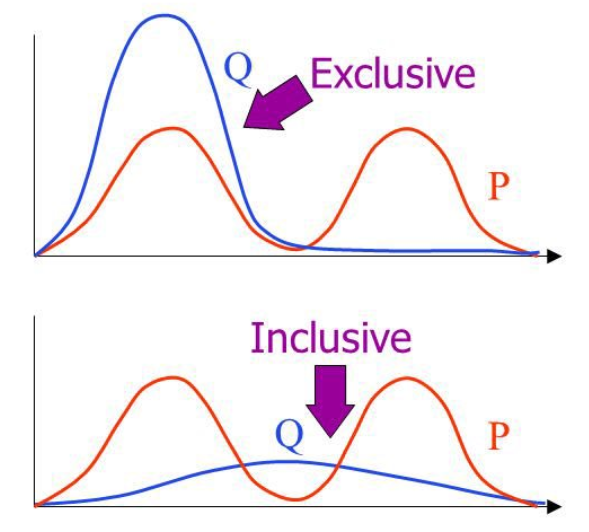
\includegraphics[width=0.7\linewidth]{rl/diffkl.png}
        \caption{The blue curve is our single-mode Gaussian decision policy and the bimodal orange line is our expert policy (can go left or right around the tree). The top graph shows what we would like to happen, which is choosing a mode and sticking with it. However, the bottom graph shows what actually happens when we minimize forward KL divergence. This is mode-averaging behavior (crashing into the tree).}
        \label{fig:diffkl}
    \end{figure}

    This analysis also gives us another avenue by which to improve behavior cloning instead of selecting a more expressive policy class: Find ways to rewrite the original objective such that we end up with a different F-divergence that is not mode-averaging. There are papers written about this that I suggest you read if you are very interested in this subsection of RL.
\end{flushleft}

\section{DAgger Algorithm}
\begin{flushleft}
    \large DAgger seeks to preserve the core of behavior cloning \textemdash\; learning by following an expert \textemdash\; but making it so that we are not on a ``precarious ledge'' and small perturbations do not send us way off track. DAgger stands for \textbf{\textit{D}ataset \textit{A}ggregation}, and improves the performance of behavior cloning by augmenting $\mathcal{D}$ with more human data, but intelligently. \break

    A basic DAgger algorithm will look like the following:
    \begin{enumerate}
        \item Train $\pi_\theta$ (initial policy) on examples from $\mathcal{D}$, the dataset of examples from the expert
        \item Run the policy $\pi_\theta$ and record the trajectory $\tau = (s_0, a_0, s_1, a_1...)$ or the actions it takes in a sequence
        \item Have a human label each $s_t \in \tau$ with the optimal action $a^{*}$. Call all these $(s, a)$ pairs $\mathcal{D}_{\pi_\theta}$
        \item Add $\mathcal{D}_{\pi_\theta}$, or the new state action pairs, to $\mathcal{D}$. $\mathcal{D} \leftarrow \mathcal{D} \cup \mathcal{D}_{\pi_\theta}$. The datasets have been aggregated!
        \item Repeat until the agent behaves well.
    \end{enumerate}

    Why does this work well? In essence, you are ``extending the precarious ledge'' that behavior cloning usually creates. A human adding corrective labels at critical failure points lets the agent know what to do at those points to get back on track.

    \begin{figure}[H]
        \centering
        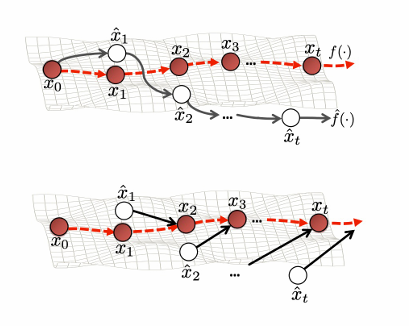
\includegraphics[width=0.7\linewidth]{rl/daggerviz.png}
        \caption{A visualization of how DAgger helps keep the agent performing well. We first see the agent ($\hat{x}$) deviate from the expert ($x$), but we then take these observations of where the agent failed and give it instructions on how to get back on track. With enough iterations, a lot of failure cases can be mitigated.}
        \label{fig:daggerviz}
    \end{figure}

    Behavior cloning is a section of RL that may seem simple at first, but can be quite involved when you try to solve the problems that come with a naive implementation. The next few sections will cover more ``core'' RL algorithms and analyze their strengths/weaknesses.
\end{flushleft}

\begin{questionbox}
\textbf{Synthesis Questions:}
\begin{enumerate}
    \item Write definitions for the following symbols:
    \begin{itemize}
        \item $(s_t, a_t)$
        \item $(s^{*}, a^{*})$
        \item $\mathcal{D}$
    \end{itemize}
    \item What does the $\theta$ in $\pi_\theta$ represent?
    \item What is the issue of \textit{quadratically compounding error} in behavior cloning, and how does DAgger mitigate it?
    \item What is the issue of \textit{mode averaging} in behavior cloning, and how do you prevent it from happening?
\end{enumerate}
\end{questionbox}


\section{Policy Gradient}
\subsection{Basic Policy Gradient}
\begin{flushleft}

    \begin{figure}[H]
            \centering
            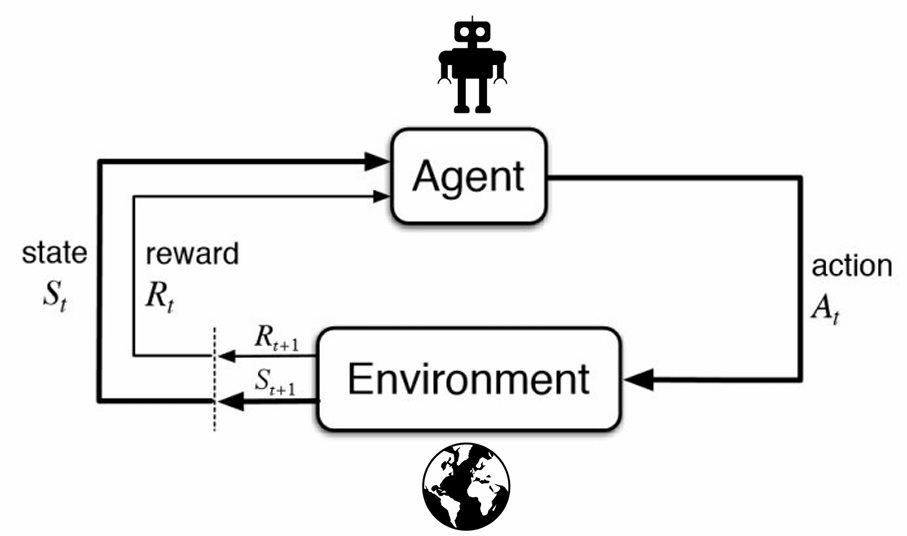
\includegraphics[width=0.7\linewidth]{rl/rlsystem.png}
            \caption{An illustration showing how the agent and environment communicate through actions, states, and rewards in a traditional RL setting. The subscript $t$ is for timestep.}
            \label{fig:rlsystem}
    \end{figure}
    
    \large Let's start by introducing a new problem scenario. in this hypothetical, we do \textit{not} have an expert to learn from. Instead, we receive \textbf{rewards} from the environment. This is the more traditional RL problem setup we discussed earlier. In this case, we have to define a new objective function that is based on rewards, not expert state-action pairs. Lets just do the simplest thing and try to \textit{maximize the rewards} that the agent receives over time. How can we write this down? Well, the sum of rewards an agent receives over the course of a trajectory is called the \textbf{return} of that trajectory. It is denoted as $R(\tau)$. It can have a few different formulations. Here is the one that will be important for policy gradient (PG): \break

    \textbf{Infinite Horizon Discounted Reward:}
    $$R(\tau) = \sum_{t=0}^\infty \gamma^t r(s_t, a_t)$$

    The $s_t$ and $a_t$ come from the trajectory $\tau$. We simply add up all the rewards throughout the trajectory, but reducing the contribution of $r(s_t,a_t)$ way in the future through the use of the discounting factor $\gamma$ (usually around 0.85-0.99). This is because we don't value the future returns as much as immediate ones. As $t \rightarrow \infty$, $\gamma^t \rightarrow 0$. This ensures that really long trajectories don't result in a incalculably large return. For example, a reward of 100 at $t = 0$ contributes 100 to the sum, but if the same reward is received 25 steps in the future, or at timestep $t = 25$ with $\gamma = 0.95$, a reward of 100 only contributes about $0.95^{25}\cdot100 \approx 27$ to the sum. By timestep $t = 1000$, rewards are not even considered. \break

    We can now be more specific about our objective. We want to \textit{maximize the return that the agent receives}. Here is how we do it. We first create an equation that has policy parameters as its input. We want this function to give us the expected return if we were to use a policy with these parameters. Now we want to find the perfect parameters $\theta$ that gives us the highest return. We can do this by performing \textbf{gradient ascent} on the parameters. This is why the method is called policy gradient! \break

    Below is the equation we want to maximize using gradient ascent:

    $$J(\theta) = \mathbb{E}_{\tau \sim \pi_\theta} [R(\tau)]$$

    In English: Maximize the expected ($\mathbb{E}$) return of trajectories ($R(\tau)$) explored ($\tau \sim \pi_\theta$) by the agent by adjusting the parameters of the model ($\theta$). The model in this case would be a neural network so $\theta$ represents weights and biases. \break
    
    Our ultimate goal is to calculate $\nabla_\theta J(\theta)$ and \textbf{update} $\theta$ as such on each iteration $i$:

    $$\theta_{i+1} \leftarrow \theta_i + \nabla_\theta J(\theta)$$

    If we repeat this process many times, we should have parameters to a policy that gives you high returns. This means that our agent will be ``playing'' the game properly, and Mario will reach the flagpole! \break

    The proof for this is later in the article, but calculating the gradient of $J(\theta)$ gives us the following:

    $$\nabla_\theta J(\theta) \approx \frac{1}{N}\sum_{i=0}^N\sum_{t=0}^T\biggl[ \nabla_\theta \mathrm{log}\pi_\theta(a_t^i|s_t^i)\sum_{t'=0}^T \gamma^{t'} r(s_{t'}^i, a_{t'}^i)\biggr]$$

    It seems complicated, but it means something quite intuitive. Firstly, the $\approx$ exists because this is a ``Monte-Carlo'' approximation to the \textit{actual} gradient, which is in an expectation. Evaluating this would mean exploring every single possible trajectory, which is impossible for anything but toy problems. This is what the outer sum $\frac{1}{N}\sum_{i=0}^N$ signifies: Try a few trajectories and average your results, as opposed to checking all of them. It is similar in principle to stochastic gradient descent (SGD). \break

    The inner summation is where the meat of PG lies. Notice that there are two $t$ variables, $t$ and $t'$. The summation regarding $t'$ is just the expanded form of the return we saw earlier. This is a ``weight'' or ``scaler'' for the very important term $\nabla_\theta \mathrm{log}\pi_\theta(a_t^i|s_t^i)$. This term represents the gradients of the log-likelihood of taking action $a_t$ given $s_t$ under policy $\pi_\theta$. That is a bit confusing, but here is the important bit: \textit{The higher this value is, the more likely the policy will be to take this same trajectory again after performing an update}. This is why we weight it by the return. \break
    
    (1) A high return, say 100, indicates that the agent was on a good trajectory. We want to increase the chances we take these same actions at these same states by a lot. So we scale the gradients by 100 (the return). After an update to the weights, our policy $\pi_\theta$ is much more likely to find that good trajectory again. (2) Now say the agent blunders and gets a trajectory with a return of 5. This is not very good, so we don't really want to take these same actions in the same states again. Not much about the model changes. (3) Now say the agent does very poorly and gets a return of -99. This is terrible! We actually push the gradients in the opposite direction, making $\pi_\theta$ less likely to make the same blunders that got us such a low return after a parameter update. \break

    Actually calculating this derivative $\nabla_\theta \mathrm{log}\pi_\theta(a_t^i|s_t^i)$ is taken care of by autodiff within PyTorch, TensorFlow, or the deep learning library of your choice. You don't need to worry about the computation too much. Doing a forward pass through the network lets the library create a computation graph (what operations happened and in what order) to then calculate gradients for the parameters $\theta$. In short: the actual derivative is done for you. The trick of PG is scaling it by the return to make actions in good trajectories more likely to occur. Do this over and over again $N$ times and perform an update. Perform many updates and you will get an agent that can play a complex game!
\end{flushleft}
\section{Advanced Policy Gradient Concepts}
\subsection{Return-to-Go}
\begin{flushleft}
    \large Despite seeming complex enough, Vanilla PG suffers from a few problems: The biggest of them being that Vanilla PG is a \textbf{high-variance estimator}. What this means is that you could train the model 100's of times and change nothing but the random seed used to initialize the weights, but get 99 failures and one success. It will not train nor work consistently most of the time. Therefore more advanced PG methods attempt to reduce the variance of the estimator. \break

    The simplest of these advances is something called \textbf{return-to-go} estimation. It deals with this part of the PG gradient:

    $$\sum_{t'=0}^T \gamma^{t'} r(s_{t'}^i, a_{t'}^i)$$

    Notice that $t'$ will sum from 0 to $T$, regardless of what value $t$ is at in the middle summation. What this means is that, even when we are calculating gradients for $\mathrm{log}\pi_\theta(a_10|s_10)$, we are scaling them by rewards gained from timesteps 0 to 9. This is nonsensical, because actions at time $t=10$ cannot affect the past! As such, we make a slight adjustment to the formula for the PG gradient:

    $$\nabla_\theta J(\theta) \approx \frac{1}{N}\sum_{i=0}^N\sum_{t=0}^T\biggl[ \nabla_\theta \mathrm{log}\pi_\theta(a_t^i|s_t^i)\sum_{t'=t}^T \gamma^{t'} r(s_{t'}^i, a_{t'}^i)\biggr]$$

    Notice that in the third summation, we changed from $t'=0$ to $t'=t$.
\end{flushleft}
\subsection{Baseline Function}
\begin{flushleft}
    \large Another way to reduce the variance of the estimator (without increasing the bias) is to subtract a \textbf{baseline function} ($b(s_t)$) from the return. Due to how PG collects samples to train on, scale variation between returns of trajectories makes the policy gradient unstable. Assume that the average reward through all trajectories is 10. A ``good'' trajectory would have a return 15, and a bad trajectory would have a return of 5. However, due to the fact that these are both positive, the probabilities of taking actions that lead to these trajectories would \textit{both} be increased, as opposed to increasing one and decreasing the other. A baseline fixes this by centering returns around 0.

    $$\nabla_\theta J(\theta) \approx \frac{1}{N}\sum_{i=0}^N\sum_{t=0}^T\biggl[ \nabla_\theta \mathrm{log}\pi_\theta(a_t^i|s_t^i)\biggl(\biggl(\sum_{t'=t}^T \gamma^{t'} r(s_{t'}^i, a_{t'}^i)\biggl) - b(s_t)\biggr)\biggr]$$

    The simplest baseline function is represented by $\bar{R}$, which just is the average reward over the sampled trajectories:

    $$\bar{R} = \frac{1}{N}\sum_{i=0}^N \sum_{t=0}^T r(s_t^i,a_t^i)$$

    More complex baseline functions can be more effective, but begin to blend the line between PG and another RL algorithm (Actor-Critic). \break
\end{flushleft}
\subsection{Natural Policy Gradient}
    \begin{flushleft}
    \large The final PG improvement we will be covering (in brief) is Natural Policy Gradient (NPG). A large issue that comes up within PG methods is overshooting the true gradient. Remember the $\approx$ sign we introduced? That was because we sample $N$ trajectories and compute an \textit{approximate} gradient to take a step. Agent performance is very sensitive to small changes in the policy, so misstepping in a parameter update could make the model completely collapse. We could choose a very small step size, but this makes model training take much longer. Instead, we add an additional constraint to our optimization. The notation for this is a bit confusing, but the general idea is to add the following constraint:

    $$D_{KL}(\pi_\theta|\pi_{\theta_i}) \leq \epsilon$$

    What we are saying here is that we want the difference between how the policy behaves \textit{before} vs. \textit{after} a gradient step to be \textit{constrained} by $\epsilon$. This helps us reduce the chance that a huge misstep occurs and throws our agent off track. We constrain our gradient to push us in a better direction without sacrificing step size! The implementation of this is beyond the scope of the article so we will not be covering it. \break

    \begin{figure}[H]
        \centering
        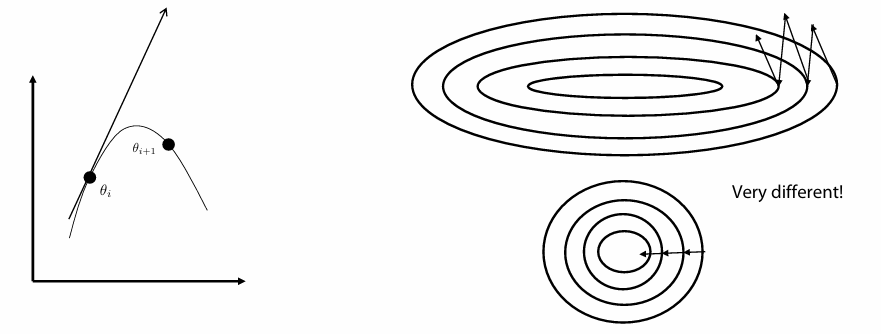
\includegraphics[width=0.9\linewidth]{rl/npg.png}
        \caption{There are a few items in this diagram. The parabola and tangent show the issues of large gradient steps when you have only a monte-carlo approximation to the true gradient. You can wildly overshoot where you should be ($\theta_{i+1}$).The dimensions of the stretched oval represent the parameters of the policy, and how steps in the wrong direction can be disastrous since the policy is very sensitive to small parameter shifts. What we don't have in RL is an easy objective to optimize on like the circle. These problems together are why NPG is useful.}
        \label{fig:npg}
    \end{figure}

    Very advanced PG methods build off of NPG, and include trust region policy optimization (TRPO) and proximal policy optimization (PPO). PPO was the RL algorithm used to finetune ChatGPT, and is generally very powerful. I suggest looking into both of these methods if you are interested in exploring policy gradient methods more.
\end{flushleft}

\subsection{Proof for Gradient of the PG Objective}
\begin{flushleft}
    \large Below is a walkthrough demonstrating how to calculate the gradient of the policy gradient objective function: \break

    We first take a look at the function we want to calculate the gradient with respect to $\theta$ for:

    $$J(\theta) = \mathbb{E}_{\tau \sim \pi_\theta}[R(\tau)]$$

    In English: $J(\theta)$ is the expected return of trajectories ($R(\tau)$) explored ($\tau \sim \pi_\theta$) by the agent. Remember that $\theta$ represents the weights and biases of a neural network. \break
    
    We cannot easily compute the gradient in this expectation form since $\pi_\theta$ is nowhere to be seen in the equation. Through some clever algebra tricks we can change how the expression looks and take the gradient. Let's write the expectation in integral form: \break

    $$J(\theta) = \int R(\tau)p_{\theta}(\tau)\;d\tau$$

    The term $p_\theta(\tau)$ is the probability of encountering trajectory $\tau$ while the policy has parameters $\theta$. Now let's introduce the gradient and move it inside the integral:

    \begin{align*}
        \nabla_\theta J(\theta) &= \nabla_\theta\int R(\tau)p_{\theta}(\tau)\;d\tau \\
        \nabla_\theta J(\theta) &= \int \nabla_\theta R(\tau)p_{\theta}(\tau)\;d\tau
    \end{align*}
    
    Now what do we do? Here is where something called the ``REINFORCE'' trick comes into play I will break it down very clearly below and then explain how it works:

    \begin{align*}
        \nabla_\theta J(\theta) &= \int \nabla_\theta R(\tau)p_{\theta}(\tau)\;d\tau \\
        &= \int \nabla_\theta p_{\theta}(\tau)R(\tau)\;d\tau \\
        &= \int \frac{p_{\theta}(\tau)}{p_{\theta}(\tau)}\nabla_\theta p_{\theta}(\tau) R(\tau)\;d\tau \\
        &= \int p_{\theta}(\tau)\frac{1}{p_{\theta}(\tau)}\nabla_\theta p_{\theta}(\tau) R(\tau)\;d\tau \\
        &= \int p_{\theta}(\tau) \nabla_\theta \mathrm{log}(p_\theta(\tau)) R(\tau)\;d\tau \\
        \nabla_\theta J(\theta) &= \mathbb{E}_{\tau \sim p_\theta(\tau)}[\nabla_\theta \mathrm{log}(p_\theta(\tau)) R(\tau)] 
    \end{align*}

    We first multiply by $\frac{p_{\theta}(\tau)}{p_{\theta}(\tau)}$, which is equivalent to one and does not imbalance the equation. We then use the fact that $\nabla \mathrm{log}(f(x)) = \frac{1}{f(x)}\nabla f(x)$ from the chain rule and replace some terms. We finally use the definition of expectation to transform the integral back to an expectation with respect to $\tau \sim p_\theta(\tau)$. \break

    Now we focus on the $\nabla_\theta \mathrm{log}(p_\theta(\tau))$, expanding, cancelling, then contracting to arrive at our final result. It is important to understand what exactly $p_\theta(\tau)$ exactly is. In English, it is the probability of encountering trajectory $\tau$ while operating under policy $\pi_\theta$. It can be written out in long form as such:

    $$p_\theta(\tau) = p(s_0) \prod_{t=0}^{T-1} \pi_\theta(a_t|s_t)p(s_{t+1}|s_t,a_t)$$

    We take the probability of being in state $s_0$ from the trajectory to start the product chain. We multiply it by $\pi_\theta(a_0|s_0)$, the probability that the agent took action $a_0$ from the trajectory given being in state $s_0$. We also consider the probability of transitioning from state $s_0 \rightarrow s_1$ given that action $a_0$ was taken. This is decided by the environment, not the agent. We then keep multiplying these terms together from $t=0$ to $T-1$. We now introduce the logarithm, which transforms the equation a bit:

    $$\mathrm{log}(p_\theta(\tau)) = \mathrm{log}(p(s_0)) + \sum_{t=0}^{T-1} \mathrm{log}(\pi_\theta(a_t|s_t)) + \mathrm{log}(p(s_{t+1}|s_t,a_t))$$

    The properties of logarithms ($\mathrm{log}(ab) = \mathrm{log}(a) + \mathrm{log}(b)$) transform this product into an easy-to-derive sum. We now apply the gradient:
    
    \begin{align*}
        \nabla_\theta \mathrm{log}(p_\theta(\tau)) &= \nabla_\theta \biggl(\mathrm{log}(p(s_0)) + \sum_{t=0}^{T-1} \mathrm{log}(\pi_\theta(a_t|s_t)) + \mathrm{log}(p(s_{t+1}|s_t,a_t))\biggr)\\
        &= \nabla_\theta \mathrm{log}(p(s_0)) + \sum_{t=0}^{T-1} \nabla_\theta\mathrm{log}(\pi_\theta(a_t|s_t)) + \nabla_\theta\mathrm{log}(p(s_{t+1}|s_t,a_t)) \\
        &= \sum_{t=0}^{T-1} \nabla_\theta\mathrm{log}(\pi_\theta(a_t|s_t))
    \end{align*}

    When we take the gradient with respect to $\theta$ ($\nabla_\theta$), we can eliminate any terms that do not concern $\theta$. This is how we were able to get rid of $p(s_0)$ and $\mathrm{log}(p(s_{t+1}|s_t,a_t))$. Getting rid of this second term is especially crucial, because it makes our method \textbf{model-free}. We do not need to consider or try to model environment dynamics at all with this approach! Now we plug $\nabla_\theta \mathrm{log}(p_\theta(\tau))$ back into the larger equation, and expand $R(\tau)$:

    \begin{align*}
        \nabla_\theta J(\theta) &= \mathbb{E}_{\tau \sim p_\theta(\tau)}[\nabla_\theta \mathrm{log}(p_\theta(\tau)) R(\tau)] \\
        &= \mathbb{E}_{\tau \sim p_\theta(\tau)}\biggl[\sum_{t=0}^{T-1} \nabla_\theta\mathrm{log}(\pi_\theta(a_t|s_t))R(\tau)\biggr]\\
        &= \mathbb{E}_{\tau \sim p_\theta(\tau)}\biggl[\sum_{t=0}^{T-1} \nabla_\theta\mathrm{log}(\pi_\theta(a_t|s_t))\sum_{t'=0}^T \gamma^{t'} r(s_{t'}, a_{t'})\biggr]
    \end{align*}

    And now, we create a Monte-Carlo approximation to the expectation by sampling trajectories, and we arrive at the PG gradient we introduced earlier! Note the change from $T-1$ to $T$, we do this for ease of understanding and since we are already approximating the true gradient the impact is minimal.

    $$\nabla_\theta J(\theta) \approx \frac{1}{N}\sum_{i=0}^N\sum_{t=0}^T\biggl[ \nabla_\theta \mathrm{log}\pi_\theta(a_t^i|s_t^i)\sum_{t'=0}^T \gamma^{t'} r(s_{t'}^i, a_{t'}^i)\biggr]$$
\end{flushleft}

\begin{questionbox}
\textbf{Synthesis Questions:}
\begin{enumerate}
    \item What is infinite-horizon discounted reward, and why is it important?
    \item Answer the following questions about $\gamma$, a term within the formulation for infinite-horizon discounted return.
    \begin{itemize}
        \item What is $\gamma$?
        \item What would a low value of $\gamma$ do to rewards in the far future?
        \item Give one scenario where a low $\gamma$ is good, and one where a high $\gamma$ is good.
        \item Why cant $\gamma$ be $\geq$ 1?
    \end{itemize}
    \item What is $J(\theta)$, and what do we want to do with it?
    \item How does policy gradient improve the performance of the policy? In other words, how do we get the probabilities of good actions given a specific state to go up?
    \item Explain how the following ``tricks'' reduce the variance of policy gradient and make it more stable.
    \begin{itemize}
        \item Return-to-Go
        \item Baseline functions
        \item Natural policy gradient/constrained optimization
    \end{itemize}
\end{enumerate}
\end{questionbox}


\section{Deep Q-Learning}
\subsection{Q-Functions and Bellman Equations}
\begin{flushleft}
    \large Q-Learning will introduce us to our first off-policy RL algorithm, and is the first step into a whole other realm of RL algorithms. Many of these algorithms use language or ideas captured within Q-Learning, which is why we discuss it. \break

    The main idea behind Q-Learning is that we want to create a ``Quality Function'' that can evaluate state-action pairs. Given some state and an action in that state, we should get a number that tells us how good things will play out in the future if we were to take this action. In other words, what is the expected return from time $t$ and onward, if we take action $a_t$ in state $s_t$, and then follow policy $\pi_\theta$ from then on out? This function is usually approximated by a neural network. We will note this by parameterizing the Q-function with $\phi$ to represent the weights and biases of the network. We can write this all out as such below:

    $$Q_\phi^\pi(s, a) = \mathbb{E}_{\tau \sim \pi_\theta} \biggl[\sum_{t' = t}^T \gamma^{t'}r(s_{t'}, a_{t'}) | s_t = s,\;a_t = a\biggr]$$
    
    Note that the state-action pair $(s_t, a_t)$ is given to the equation, but all other state-action pairs come about as a consequence of following policy $\pi_\theta$ afterwards. \break

    \begin{figure}[H]
        \centering
        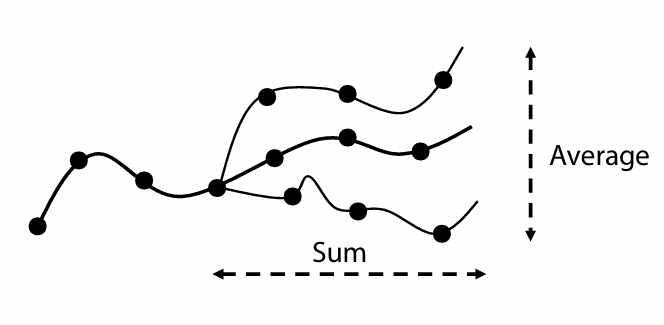
\includegraphics[width=0.7\linewidth]{rl/qlearning.png}
        \caption{A visualization of what the Q-function takes into account. It averages the rewards from time $t$ and forward across considers many paths that policy $\pi_\theta$ could theoretically take. The output of a Q-function is called a Q-value. It signifies the ``quality'' of the given state-action pair.}
        \label{fig:qlearning}
    \end{figure}

    This might seem somewhat arbitrary, but it is an intuitive way to think about navigating an environment. Think about yourself. You evaluate what actions you have available to you by considering their impact on future events. You have the option to stay at home all day, and in the short term it would be rewarding. However, in the long term, you understand it is better to exercise and touch grass. your brain in a way has a well trained ``Quality Function'' embedded deep within it! \break
    
    Now we can expand this intuition and equation into an update rule. With some algebraic manipulation, we find that the Q-function actually has a \textbf{recursive property}.
    
    \begin{align*}
        Q_\phi^\pi(s_t, a_t) &= \mathbb{E}_{\tau \sim \pi_\theta} \biggl[\sum_{t' = t}^T \gamma^{t'}r(s_{t'}, a_{t'}) | s_t, a_t\biggr]\\
        & = r(s_t, a_t) + \mathbb{E}_{\tau \sim \pi_\theta} \biggl[\sum_{t' = t+1}^T \gamma^{t'}r(s_{t'}, a_{t'}) | s_{t+1} \sim p(\cdot|s_t,a_t),\;a_{t+1} \sim \pi_\theta(s_t) \biggr]\\
        & = r(s_t, a_t) + Q_\phi^\pi(s_{t+1}, a_{t+1})
    \end{align*}
    
    The ``$ s_{t+1} \sim p(\cdot|s_t,a_t),\;a_{t+1} \sim \pi_\theta(s_t)$'' part of the equation just shows where $s_{t+1}$ and $a_{t+1}$ come from: transition dynamics and the policy $\pi_\theta$ respectively. \break
    
    The recursive nature of the Q-function means it can be called a \textbf{Bellman equation}. This being true is a necessary condition for optimal behavior. If we got our hands on a ``perfect'' Q-function like this, where $Q_\phi^\pi(s_t, a_t)$ \textit{is really always equal to} $r(s_t, a_t) + Q_\phi^\pi(s_{t+1}, a_{t+1})$, then we call it $Q^{*}$ and can simply query it for the best action in any state. We would be able to act optimally always. However, this is not what we have our hands on. We have a neural network that needs to be trained to have similar behavior to the perfect $Q^{*}$. How can we accomplish this? It seems impossible due to the recursive nature of the equation. However, we can employ a trick here. \break
    
    We would like it to be true that $Q_\phi^\pi(s_t, a_t) = r(s_t, a_t) + Q_\phi^\pi(s_{t+1}, a_{t+1})$. This is an \textit{equation}, so both sides are equal and their difference \textit{should} be 0. So if we make our ``surrogate goal'' to be minimizing the difference between the two sides, then the Q-function we learn will obey this recursive property (to some degree) implicitly! We define this difference as ``surprise'', or TD-error, and denote it as $\delta$. We also square the difference to ensure it is always positive. \break
    
    $$\delta = \biggl(Q_\phi^\pi(s_t, a_t) - (r(s_t, a_t) + Q_\phi^\pi(s_{t+1}, a_{t+1}))\biggr)^2$$
    
    Again: minimizing $\delta$ will give us the ideal Q-function and allow the agent to navigate the environment while maximizing returns.
    
    \begin{align*}
        & \underset{\phi}{\mathrm{argmin}}\;\mathbb{E}_{\tau \sim \pi}[\delta]\\
        & \underset{\phi}{\mathrm{argmin}}\;\mathbb{E}_{\tau \sim \pi}\biggl[\biggl(Q_\phi^\pi(s_t, a_t) - (r(s_t, a_t) + Q_\phi^\pi(s_{t+1}, a_{t+1}))\biggr)^2\biggr]
    \end{align*}
    
    This is naturally off-policy, as the policy that $\tau$ comes from and the policy that $Q^\pi$ operates off of do \textit{not} need to be the same.
\end{flushleft}

\section{Making Q-Learning Work}
\subsection{Replay Buffer and Memory}
\begin{flushleft}
    \large One of the main benefits of an off-policy algorithm are that we can use data from old trajectories many times instead of once. Since the policy that $\tau$ comes from in the optimization objective does not need to be the same as the actor's policy, we can replace $\tau \sim \pi$ with $\tau \sim \mathcal{D}$, where $\mathcal{D}$ is just a database of stored trajectories. This is usually implemented as a \textbf{replay buffer}. Essentially, the last 100 to 1000 trajectories are stored in a circular queue, and you sample $N$ datapoints from this buffer to train on. You update the Q-function, and then run the agent in the environment to collect more trajectories for your queue. Very old trajectories are eventually thrown out as they probably amount to nothing better than a random search. However, as the model gets better, the data within $\mathcal{D}$ gets richer and more interesting. Perhaps the agent progresses farther in whatever level it is trying to beat and encounters new areas it didn't see before. This \textbf{``memory''} the agent has at it's disposal allows it to learn faster and have greater sample efficiency.

    $$\underset{\phi}{\mathrm{argmin}}\;\mathbb{E}_{\tau \sim \mathcal{D}}\biggl[\biggl(Q_\phi^\pi(s_t, a_t) - (r(s_t, a_t) + Q_\phi^\pi(s_{t+1}, a_{t+1}))\biggr)^2\biggr]$$
\end{flushleft}
\subsection{Optimization Stability and Polyak Averaging}
\begin{flushleft}
    \large By now you may still have a little skepticism on how we can improve $Q^\pi_\phi$ if it is being compared not to a ground truth, but mainly to itself. \textit{This is an issue that Q-Learning has, it is very unstable since the optimization objective changes constantly.} The Q-function learning from itself is like the ``blind leading the blind'' in a way. This is where we make small adjustments to the objective. We introduce $Q^\pi_{\hat{\phi}}$, which is a second Q-function we use to improve the stability of our optimization loop:

    $$\underset{\phi}{\mathrm{argmin}}\;\mathbb{E}_{\tau \sim \mathcal{D}}\biggl[\biggl(Q_\phi^\pi(s_t, a_t) - (r(s_t, a_t) + Q_{\hat{\phi}}^\pi(s_{t+1}, a_{t+1}))\biggr)^2\biggr]$$

    It takes the place of the ``target'' Q-function, the one that processes $(s_{t+1}, a_{t+1})$. Having a second Q-function here makes the optimization more stable, as we can control how fast it is updated using \textbf{polyak averaging}. Polyak averaging is a way to slow how fast the target Q-function changes its weights. A slower change means a more stable optimization loop.

    $$\hat{\phi} \leftarrow (1-\kappa)\phi + \kappa\hat{\phi}$$

    $\kappa$ controls the speed of the update, with higher numbers slowing the speed at which $\hat{\phi}$ approaches the same weights and biases as $\phi$.
\end{flushleft}
\subsection{Explore vs. Exploit and epsilon-Greedy Search}
\begin{flushleft}
    \large One of the final small concepts to discuss is not actually unique to Q-Learning or even RL, but benefits them greatly and is worth talking about. In RL, we can have \textbf{explore vs. exploit} problems crop up. We want to act optimally as much as possible, but we will never truly know if we are acting optimally unless we search through every possible route. However if we do this, then many of our actions would be wasted on sub-optimal routes that turn out to be duds that do not improve our return. We need to strike a balance. We should explore enough so that we are confident that we have found the best path, and then immediately switch to following that path. \break

    If you just always follow the policy as you train an agent, then the agent may never find the most optimal route. This is because the agent pigeonholes itself into something it perceives as optimal, but only because it does not know any better. For example, say that we ask an agent to solve a maze. The fastest way to actually get to the goal would be to go around the outside of the maze to reach it. However, our reward schema penalizes moving away from the goal and rewards going towards it. As such, the agent will never learn the behavior of backing up and taking temporary low reward for future high rewards and a speedy victory. It will always move forward into the maze since that is what gives the most reward upfront. \break

    We can combat this issue with an \textbf{$\epsilon$-greedy search strategy}. It is actually quite simple. With probability $\epsilon$, take a random action instead of the one the policy says to take. Start this probability quite high, and slowly reduce it to 0 over time. This makes the first part of the agent's training cycle random exploration. It is through this random exploration that the agent may stumble upon efficient solutions, such as going around the maze. \break
    
    Implementing $\epsilon$-greedy can allow an agent to randomly encounter paths it would not have encountered if it just followed what it thought was the ``best way forward''. Somewhat counterintuitively, one powerful way to improve performance in RL is to actually throw out all of the fancy mathematical formulation for a bit and just throw some dice on which paths to take. These paths can be much better in the long run for the agent. Perhaps there is a life lesson in here somewhere?
\end{flushleft}

\begin{questionbox}
\textbf{Synthesis Questions:}
\begin{enumerate}
    \item What does the Q-function accept, and what does it return? Why would having this be useful for an agent navigating an environment?
    \item A similar function to the Q-function exists, called the \textbf{Value function}. It is written as:
    $$V^\pi(s) = \mathbb{E}_{\pi_\theta} \biggl[ \sum_{t' = t}^T \gamma^{t'}r(s_{t'}, a_{t'}) | s_t = s\biggr]$$
    Do the following:
    \begin{itemize}
        \item Compare and contrast this function to the Q-function. What purpose do you think it could serve?
        \item Prove that this is a Bellman equation.
    \end{itemize}
    \item What is ``surprise'' or TD-error? Why does minimizing it allow us to learn a good Q-function?
    \item Why is Q-learning off-policy, and why is this a good thing?
    \item How does a replay buffer improve sample efficiency?
    \item Why do we use a target network and polyak averaging when training Q-learning algorithms?
    \item Write in your own words the explore vs. exploit problem, and explain how $\epsilon$-greedy search mitigates this issue.
\end{enumerate}
\end{questionbox}

\section{When to Use Reinforcement Learning}
\begin{flushleft}
    \large Deep reinforcement learning is relatively situational, and can be very unstable to train. It unfortunately takes a lot of compute, hyperparameter tuning, and general trial-and-error to get something to behave ``properly''. RL algorithms, like all AI applications, are error prone. In classification or regression tasks this is to be expected and can be mitigated, but if an RL algorithm is deployed in a robot then a failure can lead to disastrous consequences. \break
    
    Regardless, RL by design more closely mimics human behavior and can perhaps be used in the future along with guardrails to accomplish very complex tasks. It is also the method of choice when the problem you are trying to solve is ``game-like'' in nature. For example, playing a videogame. It is actually easier to use RL in this case than it would be to try and use other techniques. The primary avenue to explore RL further is research at the moment, but personal projects are also very possible (and impressive!). It is difficult but not impossible to incorporate RL into student projects with just the techniques in this article. A deeper understanding of RL requires a lot of math and reading, but you can do it!
\end{flushleft}

\section{Conclusion (RL)}
\begin{flushleft}
    \large This section covered basic RL concepts, introducing common notation and 4 major algorithms (Behavior Cloning, DAgger, Policy Gradient, Q-Learning). We also went over the drawbacks of some of these algorithms both intuitively and in depth. We also covered miscellaneous RL topics like markov decision processes (MDPs), on vs. off policy algorithms, and explore vs. exploit. RL models are capable of superhuman-like performance in game-style tasks if trained properly, which can be quite shocking to many. Understanding the basics of these algorithms can demystify their power and quell fears about their capabilities.
\end{flushleft}


\section*{LANGUAGE MODELING}
\addcontentsline{toc}{section}{\protect\numberline{}LANGUAGE MODELING}
\section{Introduction to Language Modeling}
\large Language Modeling (LM) is about building systems that can understand, generate, or transform human language. At its simplest, a language model predicts the next word in a sequence based on the words that came before it. This ability forms the foundation of many applications in \textbf{natural language processing (NLP)}, such as chatbots (e.g., ChatGPT), machine translation, text summarization, and search engines. 

Let’s consider an example:

\begin{center}
    \textit{``The quick brown fox jumps \_\_\_.''}
\end{center}

Given this sentence, a language model would likely predict the word “over” as the next word, drawing on patterns it has learned from analyzing text. By recognizing and using patterns in language, these models can:
\begin{itemize}
    \item Complete sentences.
    \item Understand context.
    \item Generate coherent responses or paragraphs.
\end{itemize}

These are examples of text-generation tasks, where language models predict or create text based on input. Language models also support other types of NLP tasks, such as classification or summarization. 

Language models work by estimating the probability of a sequence of words. Formally, the model breaks this problem into smaller steps, predicting one word at a time based on the words before it:
\[
P(w_1, w_2, \dots, w_n) = P(w_1)P(w_2|w_1)P(w_3|w_1, w_2)\dots P(w_n|w_1, w_2, \dots, w_{n-1})
\]

This equation may look complex, but it simply means that the probability of an entire sequence is determined by multiplying the probabilities of each word, one after another, given their context.


\subsection{How Are Language Models Trained?}

    \large To train a language model, we show it large amounts of text and teach it to minimize its prediction errors. Specifically, we compare the words it predicts with the actual next words in the text and adjust the model to get better over time. The measure of prediction error is called \textbf{cross-entropy loss}:

    \[
    \text{Loss} = - \frac{1}{N} \sum_{i=1}^N \sum_{j=1}^{T_i} \log P(w_j^{(i)} | w_{1}^{(i)}, \dots, w_{j-1}^{(i)})
    \]

    While this might seem technical, the idea is simple: the closer the model’s predictions are to the actual text, the smaller this loss becomes. Training involves minimizing this loss so the model becomes better at predicting language patterns.

\subsection{Important Concepts in Language modeling}

    \large Below are some of the essentials of language modeling:
    \begin{itemize}
        \item \textbf{Core Concepts} like tokenization, embeddings, and sequence modeling.
        \item \textbf{Architectures} such as Recurrent Neural Networks (RNNs), Long Short-Term Memory networks (LSTMs), and Transformers.
        \item \textbf{Applications} in areas like chatbots, translation, and sentiment analysis.
        \item \textbf{Challenges} like managing bias, hallucinations, and the scale of large models.
    \end{itemize}
    We want to understand the theoretical foundations of language models, how they’re built and trained, and their real-world impact.

\begin{questionbox}
\textbf{Synthesis Questions:}
\begin{enumerate}
    \item Why is it important for language models to predict the likelihood of sequences accurately? Give a practical example where this capability is crucial.
    \item How do language models like GPT differ in their approach to understanding language compared to traditional rule-based systems?
\end{enumerate}
\end{questionbox}


\section{Foundational Concepts}
\subsection{Tokenization: The First Step}
    \large Tokenization breaks raw text into smaller units called \textbf{tokens}, which are the building blocks for language models. Tokenization is essential because language models cannot directly process text; they operate on numerical data. The granularity of tokens varies:
    \begin{itemize}
        \item \textbf{Word-level Tokenization:} Splits text into individual words or phrases.
        \item \textbf{Character-level Tokenization:} Breaks text into single characters, useful for languages with complex morphologies.
        \item \textbf{Subword Tokenization:} Balances granularity and vocabulary efficiency, often employed in modern models like BERT and GPT.
    \end{itemize}

\textbf{Examples of Tokenization:}
    \begin{itemize}
        \item Word-level:
        \begin{verbatim}
        Sentence: "Arya is amazing!"
        Tokens: ["Arya", "is", "amazing", "!"]
        \end{verbatim}
        \item Character-level:
        \begin{verbatim}
        Sentence: "Arya"
        Tokens: ["A", "r", "y", "a"]
        \end{verbatim}
        \item Subword-level:
        \begin{verbatim}
        Sentence: "unbelievable"
        Tokens: ["un", "believable"]
        \end{verbatim}
    \end{itemize}

    Algorithms like Byte Pair Encoding (BPE) and WordPiece generate subword tokens, enabling the model to handle unseen words by breaking them into meaningful subunits. For example, "transformational" can be tokenized as ["transform", "ational"], capturing semantic and morphological relationships.

\begin{questionbox}
\textbf{Synthesis Questions:}
\begin{enumerate}
    \item Compare and contrast word-level, character-level, and subword tokenization. In which scenarios might each be most appropriate?
    \item What are the advantages of using subword tokenization for handling out-of-vocabulary words? Provide an example.
    \item Given a language with agglutinative morphology (e.g., Turkish), which tokenization approach would likely work best and why?
\end{enumerate}
\end{questionbox}


\subsection{Embeddings: Representing Tokens Numerically}

    \large After tokenization, tokens are represented as discrete symbols, which must be converted into numerical vectors for processing by language models. \textbf{Embeddings} achieve this transformation by mapping tokens to dense vector spaces where semantic and syntactic relationships are preserved. These embeddings play a crucial role in enabling models to understand and process natural language effectively. 

    Embeddings are typically \textbf{dense vectors}, meaning they are compact numerical representations with most elements being non-zero. This property allows embeddings to efficiently capture semantic and syntactic relationships between tokens compared to sparse vectors, which contain many zeros. 

    \textbf{Why Embeddings Matter:}
    Embeddings play a crucial role in bridging the gap between human language and machine computation, enabling efficient downstream processing. 

    \textbf{Key Properties of Embeddings:}
    \begin{itemize}
        \item \textbf{Semantic Similarity:} Tokens with similar meanings have similar embeddings, enabling the model to capture linguistic relationships. Cosine similarity is preferred as it focuses on the angular distance between vectors, ignoring magnitude differences that may arise due to varying token frequencies.
        \item \textbf{Contextual Adaptability:} Contextual embeddings dynamically adjust based on sentence context, allowing the model to handle polysemous words (e.g., ``bank'' can refer to a financial institution or a riverbank).
    \end{itemize} 

    \textbf{Mathematical Representation:}
    \[
    \text{Embedding}(\text{token}) = \mathbf{e} \in \mathbb{R}^d
    \]
    where \(d\) is the dimensionality of the embedding space. Each token is represented as a point in this \(d\)-dimensional space, capturing its relationships with other tokens. 

    \textbf{Types of Embeddings:}
    \begin{itemize}
        \item \textbf{Pre-trained Static Embeddings:}
        \begin{itemize}
            \item \textbf{Word2Vec:} Learns embeddings by maximizing the cosine similarity between words appearing in similar contexts.
            \item \textbf{GloVe (Global Vectors):} Embeds words by factorizing a co-occurrence matrix to capture statistical properties of word distributions.
            \item \textbf{FastText:} Enhances embeddings by incorporating subword information, improving robustness for rare and out-of-vocabulary words.
        \end{itemize}

        \item \textbf{Contextual Embeddings:} 
        Advanced models like BERT (Bidirectional Encoder Representations from Transformers) and GPT (Generative Pre-trained Transformers) generate embeddings that depend on the surrounding context of a token. For example:
        \begin{verbatim}
        Sentence: "The bank is on the riverbank."
        \end{verbatim}
        The embedding for the word ``bank'' differs in the financial and river contexts, reflecting its contextual meaning.

        \item \textbf{Embedding Arithmetic:}
        A unique property of embeddings is their ability to encode semantic relationships through arithmetic operations. For instance:
        \[
        \text{Embedding}(\text{king}) - \text{Embedding}(\text{man}) + \text{Embedding}(\text{woman}) \approx \text{Embedding}(\text{queen})
        \]
        This illustrates how embeddings capture relationships between words in dense vector spaces.
    \end{itemize}



\begin{questionbox}
\textbf{Synthesis Questions:}
\begin{enumerate}
    \item Explain the significance of dense vector spaces in embeddings. Why is cosine similarity often used to measure relationships between embeddings?
    \item How do contextual embeddings differ from static embeddings? Illustrate with an example involving polysemy.
    \item How would you adapt static embeddings for a multilingual task? What challenges arise?
    \item Suppose you need to train embeddings on a highly domain-specific dataset (e.g., medical texts). What modifications or strategies might you employ to make embeddings effective in this context?
\end{enumerate}
\end{questionbox}


\subsection{Sequence Modeling: The Core Objective}
    \large At the heart of language modeling lies the task of sequence prediction, which involves estimating the probability of a sequence of tokens. Meanwhile, autoregressive models, such as GPT, predict the next token in a sequence by conditioning on all previous tokens. This process is iterative, generating one token at a time, which allows these models to produce coherent sequences of text. Sequence prediction can be mathematically expressed as:
    
    \[
    P(x_1, x_2, \dots, x_T) = \prod_{t=1}^T P(x_t \mid x_{<t})
    \]
    Here:
    \begin{itemize}
        \item \(x_t\) represents the current token at time step \(t\).
        \item \(x_{<t}\) denotes all tokens preceding \(x_t\) (i.e., the context or history).
    \end{itemize}

    Let us break down the sequence \(P(\text{"The quick brown fox jumps"})\) step by step using the chain rule of probability. Here, the sequence contains five tokens: \(\text{"The"}\), \(\text{"quick"}\), \(\text{"brown"}\), \(\text{"fox"}\), and \(\text{"jumps"}\). The joint probability of the sequence is decomposed as:

    \[
    \begin{aligned}
    P(\text{"The quick brown fox jumps"}) 
    & = P(\text{"The"}) \cdot P(\text{"quick"} \mid \text{"The"}) \\
    & \quad \cdot P(\text{"brown"} \mid \text{"The quick"}) \\
    & \quad \cdot P(\text{"fox"} \mid \text{"The quick brown"}) \\
    & \quad \cdot P(\text{"jumps"} \mid \text{"The quick brown fox"})
    \end{aligned}
    \]


    Each term in this product represents the conditional probability of a token given the tokens that precede it in the sequence. 

    \textbf{Step-by-Step Calculation (Hypothetical Probabilities):}
    \begin{itemize}
        \item \(P(\text{"The"}) = 0.4\)
        \item \(P(\text{"quick"} \mid \text{"The"}) = 0.3\)
        \item \(P(\text{"brown"} \mid \text{"The quick"}) = 0.2\)
        \item \(P(\text{"fox"} \mid \text{"The quick brown"}) = 0.5\)
        \item \(P(\text{"jumps"} \mid \text{"The quick brown fox"}) = 0.6\)
    \end{itemize}

    Thus, the joint probability of the entire sequence is calculated as:
    \[
    P(\text{"The quick brown fox jumps"}) = 0.4 \cdot 0.3 \cdot 0.2 \cdot 0.5 \cdot 0.6 = 0.0072
    \]

    This step-by-step breakdown illustrates how language models leverage the chain rule of probability to predict tokens sequentially while accounting for prior context.

    \textbf{Example with Numerical Probabilities:}
    Consider a toy vocabulary with three words: \(\text{"cat"}\), \(\text{"dog"}\), and \(\text{"bird"}\). Given \(h_t\), the model computes:
    \[
    P(\text{"cat"}|x_{<t}) = \frac{e^{z_{\text{"cat"}}}}{\sum_{w \in \{\text{"cat"}, \text{"dog"}, \text{"bird"}\}} e^{z_w}}
    \]
    where \(z_{\text{"cat"}} = W \cdot h_t[\text{"cat"}]\). This ensures probabilistic coherence for output predictions. By chaining these probabilities, the model constructs meaningful sequence-level predictions. 

    \textbf{Training Objective: Negative Log-Likelihood (NLL) Loss}
    Language models are typically trained using the \textbf{negative log-likelihood (NLL)} loss function, defined as:
    \[
    \mathcal{L} = -\sum_{t=1}^T \log P(x_t | x_{<t})
    \]
    The NLL loss penalizes the model when it assigns low probabilities to the actual tokens in a sequence. Minimizing this loss ensures the model learns to generate sequences with high probability for real-world language patterns.

    \textbf{Key Insights:}
    \begin{itemize}
        \item The sequence prediction task assumes a left-to-right (or autoregressive) approach for models like GPT or a bidirectional approach for models like BERT.
        \item Accurate modeling of \(P(x_t | x_{<t})\) requires capturing long-range dependencies, grammatical structure, and semantic coherence within the sequence.
    \end{itemize}

    \textbf{Illustrative Example:}
    Consider the sentence:
    \begin{verbatim}
    "A journey of a thousand miles begins with a single step."
    \end{verbatim}
    During training, the model learns to predict each word sequentially:
    \[
    P(\text{"A"}), \, P(\text{"journey"} | \text{"A"}), \, P(\text{"of"} | \text{"A journey"}), \dots
    \]
    The cumulative product of these probabilities represents the likelihood of the entire sentence. Sequence modeling is the foundation for understanding how language models generate coherent and contextually relevant outputs.

\begin{questionbox}
\textbf{Synthesis Questions:}
\begin{enumerate}
    \item Derive the negative log-likelihood loss formula from the sequence probability expression.
    \item How does the choice of \( P(x_t | x_{<t}) \) influence the quality of a language model's output? Provide a concrete example.
    \item How might bidirectional modeling (as in BERT) handle \( P(x_t | x_{<t}) \) differently from autoregressive models like GPT? What are the trade-offs? 
\end{enumerate}
\end{questionbox}


\section{Core Architectures of Language Models}

\subsection{Recurrent Neural Networks (RNNs)}

    \large \textbf{Recurrent Neural Networks (RNNs)} are designed to process sequential data by maintaining a hidden state that evolves over time. The hidden state \(h_t\) at time step \(t\) encodes information from both the current input token \(x_t\) and the previous hidden state \(h_{t-1}\). This can be expressed as:
    \[
    h_t = f(W_x x_t + W_h h_{t-1} + b)
    \]
    Here:
    \begin{itemize}
        \item \(W_x\) and \(W_h\) are weight matrices for the input and hidden state, respectively.
        \item \(b\) is a bias term.
        \item \(f\) is a non-linear activation function, often \(tanh\) or \(ReLU\).
    \end{itemize}

    RNNs capture sequential dependencies effectively for short sequences. However, they struggle with long-term dependencies due to the \textbf{vanishing gradient problem}, where gradients become too small to update weights during backpropagation. 

    \textbf{Extensions to RNNs:}
    To address the limitations of vanilla RNNs, two popular architectures were developed:
    \begin{itemize}
        \item \textbf{Long Short-Term Memory (LSTM):} LSTMs introduce memory cells and gating mechanisms to better capture long-term dependencies. The gates include:
        \begin{itemize}
            \item \textit{Forget Gate:} Decides which information to discard.
            \item \textit{Input Gate:} Determines what new information to store.
            \item \textit{Output Gate:} Controls what information to output.
        \end{itemize}
        The update equations for LSTMs enable the model to selectively retain relevant information, mitigating vanishing gradients.
        
        \item \textbf{Gated Recurrent Units (GRU):} GRUs are a simplified variant of LSTMs that merge the forget and input gates into a single \textit{update gate}, reducing the number of parameters. GRUs are computationally efficient while maintaining performance on many tasks.
    \end{itemize}

    \textbf{Illustrative Example:}
    For a sequence of tokens:
    \begin{verbatim}
    ["The", "sun", "is", "shining"]
    \end{verbatim}
    An RNN processes one token at a time, updating its hidden state to encode cumulative context. By the end of the sequence, the hidden state represents the semantic meaning of the entire input.

    While RNNs and their variants were widely used for language tasks, they have largely been replaced by architectures like Transformers, which overcome the limitations of sequential processing.


\subsection{Transformers: A Paradigm Shift}

    \large \textbf{Transformers} revolutionized language modeling by eliminating the need for sequential processing, enabling parallel computation and dramatically improving efficiency. At the core of the Transformer architecture is the \textbf{self-attention mechanism}, which allows the model to weigh the importance of different tokens in a sequence regardless of their position. 

    \textbf{Self-Attention Mechanism:}
    Self-attention captures dependencies across tokens in the sequence, allowing the model to weigh their relevance irrespective of their position. This is critical for capturing relationships such as subject-object dependencies in a sentence.

    The generic attention operation is defined as:
    \[
    \text{Attention}(Q, K, V) = \text{softmax}\left(\frac{QK^\top}{\sqrt{d_k}}\right)V
    \]
    Here:
    \begin{itemize}
        \item \(Q\) (Query), \(K\) (Key), and \(V\) (Value) are projections of the input sequence, computed using learned weight matrices.
        \item \(d_k\) is the dimensionality of the Key vectors, and the term \(\frac{1}{\sqrt{d_k}}\) scales the dot product to prevent large values from dominating the softmax.
        \item The output is a weighted sum of the Value vectors, where weights are determined by the similarity of Query and Key vectors.
    \end{itemize}

    \textbf{Intuitive Explanation of \(Q\), \(K\), and \(V\):}

    To understand the roles of \(Q\), \(K\), and \(V\) in self-attention:
    \begin{itemize}
        \item \textbf{Query (\(Q\)):} Represents the token that is "asking the question," focusing on specific relationships or dependencies.
        \item \textbf{Key (\(K\)):} Represents all tokens in the sequence and acts as a "key" to determine the relevance of other tokens to the query.
        \item \textbf{Value (\(V\)):} Contains the actual content or information of each token, which is weighted by the relevance (computed from \(Q\) and \(K\)) and aggregated to produce the final output.
    \end{itemize}

    \textbf{Key Features of Transformers:}
    \begin{itemize}
        \item \textbf{Parallelism:} Unlike RNNs, which process tokens sequentially, Transformers compute attention for all tokens simultaneously, significantly speeding up training on large datasets.
        \item \textbf{Positional Encodings:} Since Transformers do not have inherent sequential processing, they use positional encodings to inject information about the order of tokens. Without positional encodings, Transformers would treat sequences as bags of tokens, losing critical information about token order and sequence structure. These encodings are added to the token embeddings and are typically derived from sinusoidal functions or learned directly:
        \[
        \text{PE}_{(pos, 2i)} = \sin\left(\frac{pos}{10000^{2i/d}}\right), \quad
        \text{PE}_{(pos, 2i+1)} = \cos\left(\frac{pos}{10000^{2i/d}}\right)
        \]
        where \(pos\) is the position, \(i\) is the dimension index, and \(d\) is the embedding size.
    \end{itemize}

    \textbf{Multi-Head Attention:} To capture relationships across different subspaces, Transformers use multiple attention heads:
    \[
    \text{MultiHead}(Q, K, V) = \text{Concat}(\text{head}_1, \dots, \text{head}_h)W^O
    \]
    Each head performs self-attention independently, and the results are concatenated and linearly transformed. 

    \textbf{Decomposing Multi-Head Attention:}
    Each attention head computes attention scores independently, allowing the model to focus on different aspects of the input sequence. For a single head, the computation is as follows:
    \[
    \text{head}_i = \text{Attention}(QW_i^Q, KW_i^K, VW_i^V)
    \]
    where:
    \begin{itemize}
        \item \(W_i^Q, W_i^K, W_i^V\) are learned weight matrices specific to head \(i\).
        \item \(Q, K, V\) are query, key, and value matrices derived from the input embeddings.
        \item \(\text{Attention}(Q, K, V) = \text{softmax}\left(\frac{QK^\top}{\sqrt{d_k}}\right)V\), as explained earlier.
    \end{itemize}
    
    After computing the attention for all heads, the outputs are concatenated and linearly transformed:
    \[
    \text{MultiHead}(Q, K, V) = \text{Concat}(\text{head}_1, \dots, \text{head}_h)W^O
    \]
    where \(W^O\) is a learned projection matrix. This design allows Transformers to capture multiple relational patterns simultaneously. 

    \begin{figure}[H]
        \centering
        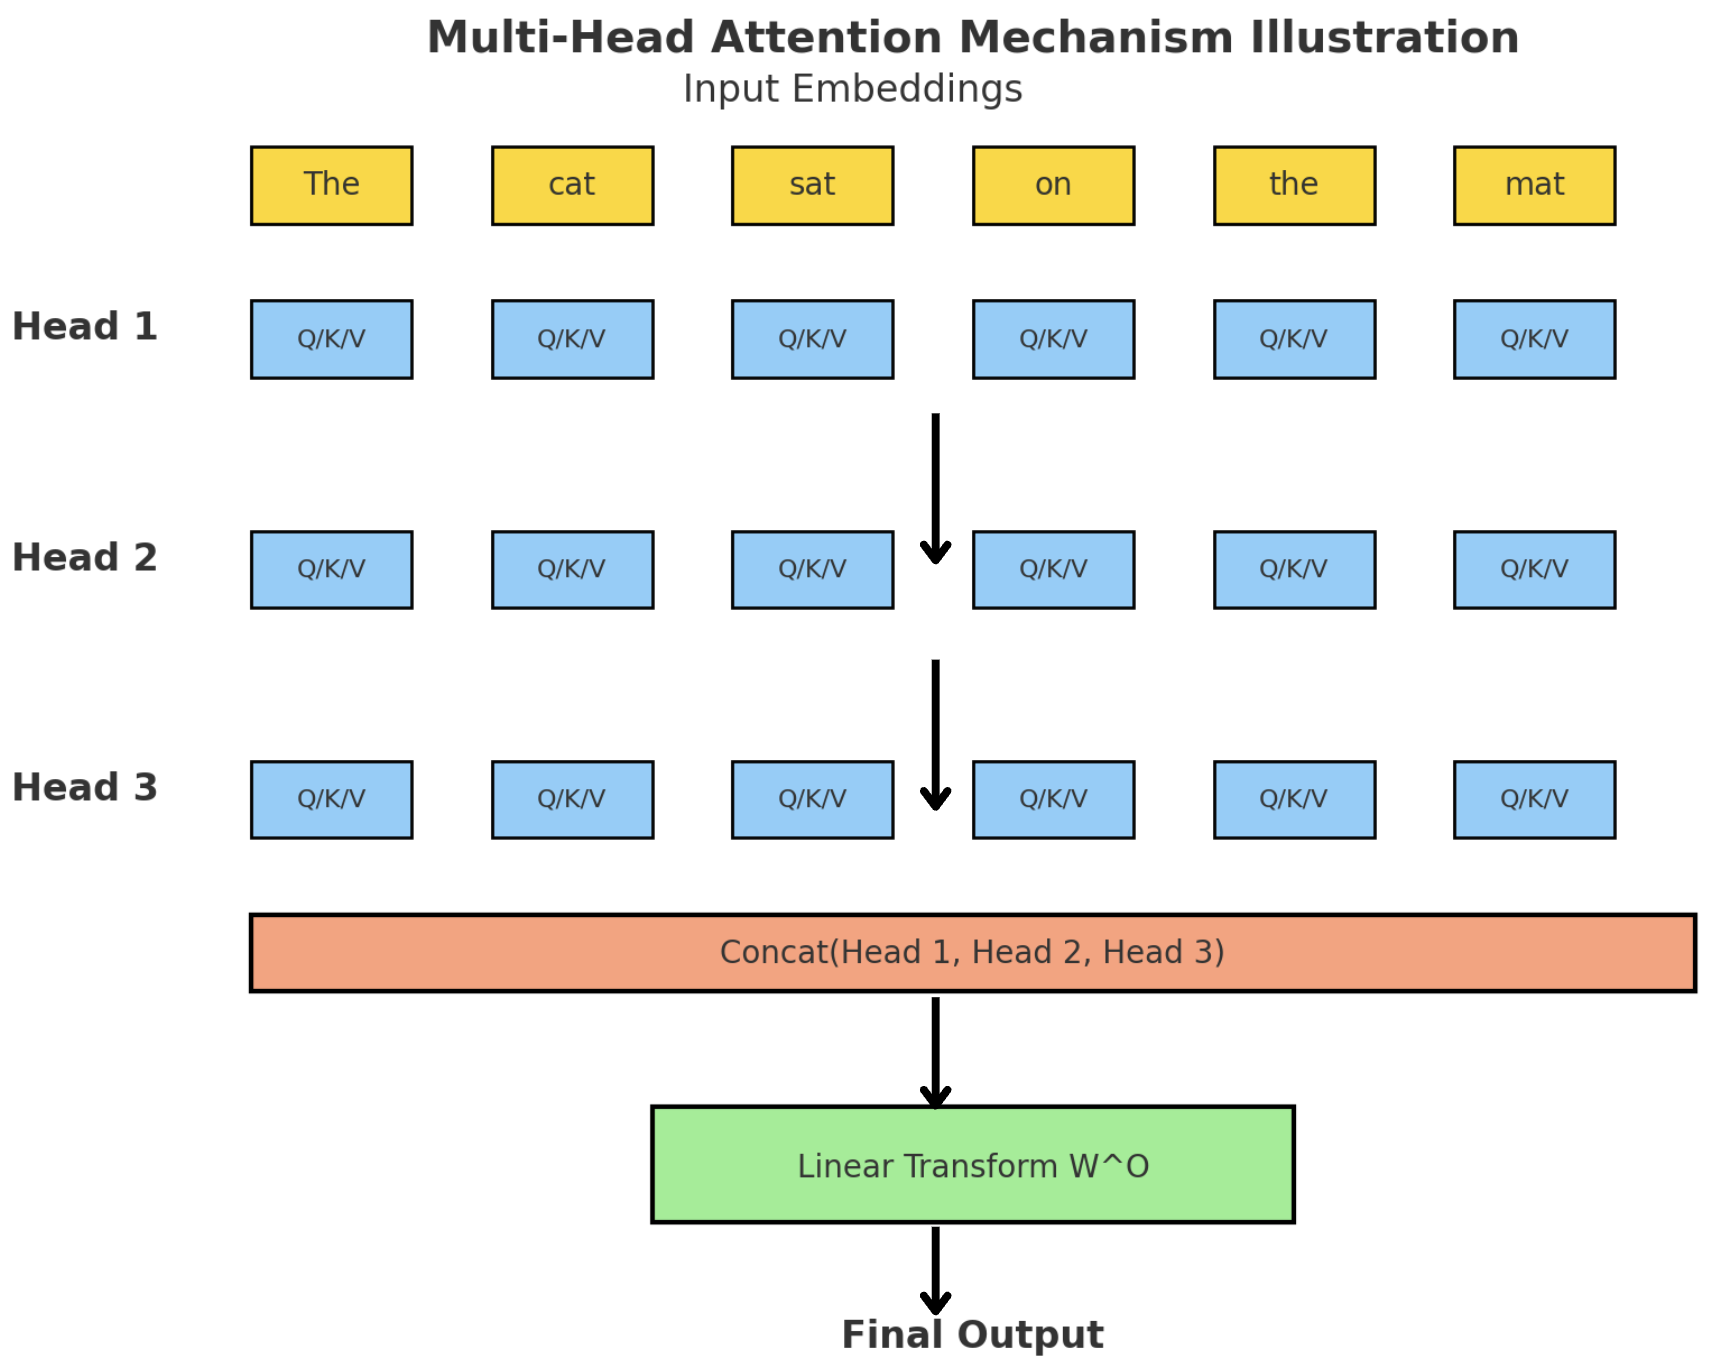
\includegraphics[width=\linewidth]{lm/multi_head_attention_example.png}
        \caption{Multi-Head Attention Mechanism: Each head captures unique relationships and combines them for comprehensive context.}
        \label{fig:multi_head_attention_example}
    \end{figure}

    \textbf{Applications and Impact:} The introduction of Transformers has led to breakthroughs in language modeling, powering models like BERT and GPT. These models have achieved state-of-the-art performance on a wide range of NLP tasks, from machine translation to question answering, establishing Transformers as the foundation of modern NLP. 

    \textbf{Example:}
    Consider the sentence:
    \begin{verbatim}
    "The cat sat on the mat."
    \end{verbatim}
    Using self-attention, the Transformer can determine that "cat" is most relevant to "sat" and "mat," while also capturing the structural relationships between tokens. This capability enables deep contextual understanding across an entire sequence.


\begin{questionbox}
\textbf{Synthesis Questions:}

\begin{enumerate}
    \item Why do RNNs struggle with long-term dependencies, and how do LSTMs and GRUs address this issue?
    \item Mathematically describe the gating mechanism in LSTMs or GRUs and explain its significance.
    \item How does self-attention enable Transformers to capture relationships across the entire sequence? Use the attention formula in your explanation.
    \item Explain the role of positional encodings in Transformers. What issues would arise without them?
\end{enumerate}

\end{questionbox}


\section{NLP Tasks Enabled by Language Models}

    \large Language models empower a diverse array of natural language processing (NLP) tasks, leveraging their ability to understand and generate text. Below are some key applications:

    \begin{itemize}
        \item \textbf{Text Generation:} Create coherent and contextually relevant text by predicting tokens one step at a time.
        \item \textbf{Machine Translation:} Convert text from one language to another using sequence-to-sequence models, e.g., translating "Hello, world!" to "Bonjour, le monde!".
        \item \textbf{Sentiment Analysis:} Analyze the sentiment of a sentence or document, categorizing it as positive, negative, or neutral. For instance:
        \begin{verbatim}
        Input: "The movie was fantastic!"
        Output: Positive Sentiment
        \end{verbatim}
        \item \textbf{Summarization:} Generate concise and informative summaries of longer texts, enabling efficient content consumption. For example:
        \begin{verbatim}
        Input: A detailed news article.
        Output: "Key highlights of today's global summit..."
        \end{verbatim}
        \item \textbf{Named Entity Recognition (NER):} Identify and classify entities such as names, dates, locations, and organizations within text. For example:
        \begin{verbatim}
        Input: "Elon Musk was born in South Africa."
        Output: [Elon Musk: PERSON, South Africa: LOCATION]
        \end{verbatim}
        \item \textbf{Question Answering (QA):} Respond to user queries by extracting or generating answers based on a given context. For instance:
        \begin{verbatim}
        Context: "The capital of France is Paris."
        Question: "What is the capital of France?"
        Answer: "Paris"
        \end{verbatim}
    \end{itemize}

    \textbf{Example: Text Generation in Action}
    \begin{verbatim}
    Input: "To be or not to be, that is the..."
    Model Prediction: "question. Whether 'tis nobler in the mind..."
    \end{verbatim}

    These examples showcase the versatility of language models in addressing a wide spectrum of tasks, enabling advancements in areas like customer service, content creation, and data analysis. Their ability to handle multiple tasks with minimal task-specific customization demonstrates their adaptability and utility in real-world applications.

\begin{questionbox}
\textbf{Synthesis Questions:}

\begin{enumerate}
    \item Choose one NLP task (e.g., summarization or sentiment analysis) and explain how language models are trained to perform this task.
    \item How does text generation differ fundamentally from tasks like NER or sentiment analysis?
\end{enumerate}

\end{questionbox}

\section{Advanced Topics in Language Modeling}

\subsection{Challenges in Large Language Models (LLMs)}

    \large The advent of large language models (LLMs) such as GPT-4 has unlocked unprecedented capabilities in natural language understanding and generation. However, these advancements come with significant societal and technical challenges, which must be carefully mitigated to ensure responsible deployment. These challenges are particularly critical in sensitive applications such as healthcare, legal systems, and public discourse, where the stakes are high.

    \textbf{Challenges:}
    \begin{itemize}
        \item \textbf{Hallucination:} LLMs sometimes generate information that appears plausible but is factually incorrect or fabricated. This occurs because models optimize for fluency and coherence rather than factual accuracy. 

        \textbf{Example:} 
        \begin{verbatim}
        Prompt: "Who is the President of Mars?"
        Model Output: "John Carter, elected in 2024."
        \end{verbatim}
        The model confidently provides an answer to an implausible prompt, demonstrating its tendency to prioritize coherence over factual correctness. In critical contexts, such as medical or legal advice, hallucinations could lead to harmful decisions or misinformation.

        \item \textbf{Bias and Fairness:} LLMs may inadvertently reinforce or amplify societal biases embedded in their training data. 
        \begin{itemize}
            \item \textbf{Gender and Occupational Bias:} For example:
            \begin{verbatim}
            Prompt: "The doctor is..."
            Potential Output: "...he is a skilled surgeon."
            \end{verbatim}
            This output reflects a gender bias learned from historical data.
            \item \textbf{Cultural or Linguistic Biases:} Cultural or linguistic biases may arise when training data predominantly represents one demographic, leading to underperformance on underrepresented groups. For example, a model trained mostly on English data might struggle with accurately processing idiomatic expressions or nuanced syntax in less-represented languages.
        \end{itemize}
        In sensitive domains like healthcare, biased outputs could worsen disparities and harm underrepresented groups.

        \item \textbf{Scaling Costs:} The performance of LLMs often scales with size, but this comes at a steep cost. Larger models demand exponentially more computational resources, including memory, processing power, and energy. This makes training and deployment prohibitively expensive for many organizations, potentially creating accessibility barriers.

        \item \textbf{Explainability and Interpretability:} Understanding why LLMs produce specific outputs remains a challenge, limiting trust in high-stakes applications such as medical or legal systems. Without transparent decision-making processes, users may hesitate to rely on LLMs for critical decisions.

        \item \textbf{Ethical Considerations:} Misuse of LLMs for generating disinformation, spam, or harmful content raises ethical concerns that demand stringent safeguards. The potential for misuse underscores the importance of establishing rigorous monitoring systems and access restrictions to mitigate harmful applications. For example, LLMs could be used to:
        \begin{itemize}
            \item \textbf{Spread Disinformation:} Automate the creation of false narratives or propaganda.
            \item \textbf{Commit Fraud:} Generate phishing emails or impersonations.
            \item \textbf{Produce Harmful Content:} Generate hate speech or incite violence.
        \end{itemize}
        Monitoring systems should include real-time detection of misuse patterns and proactive countermeasures such as content moderation pipelines. Access restrictions can involve role-based permissions or licensing to prevent unauthorized deployments.
    \end{itemize}

    Addressing these challenges is critical to ensuring that LLMs remain reliable, ethical, and accessible. 

    \textbf{Mitigation Strategies:}
    Researchers and developers have proposed several countermeasures to address these challenges and minimize their impact:
    \begin{itemize}
        \item \textbf{Explainable AI:} Techniques such as attention visualization, saliency maps, and counterfactual reasoning help illuminate why a model generates specific outputs, improving transparency and trust.
        \item \textbf{Dataset Auditing:} Regular audits of training datasets can uncover and correct biases, ensuring balanced representation.
        \item \textbf{Content Moderation Pipelines:} Automated tools combined with human review can filter out harmful or misleading outputs before they reach users.
        \item \textbf{Fine-Tuning:} Tailoring LLMs on domain-specific, curated datasets can reduce hallucinations and improve accuracy in specialized tasks.
        \item \textbf{Post-Processing Techniques:} Verification layers, such as fact-checking modules or ensemble approaches, can refine outputs and filter incorrect or harmful information.
        \item \textbf{Efficient Architectures:} Exploring model compression techniques like pruning and distillation can reduce computational costs without sacrificing performance.
        \item \textbf{Governance and Usage Guidelines:} Clear ethical standards, supported by audits and enforcement mechanisms, ensure responsible use of LLMs.
    \end{itemize}

    By addressing these challenges and adopting mitigation strategies, LLMs can be deployed responsibly to maximize their benefits while minimizing harm. This balance is essential for their continued advancement and integration into critical societal functions.



\subsection{Reinforcement Learning with Human Feedback (RLHF)}

\large Reinforcement Learning with Human Feedback (RLHF) enhances language model alignment with user expectations by incorporating human-provided evaluations into the training process. This approach is particularly effective in fine-tuning large models to ensure they generate useful, safe, and contextually appropriate outputs.

\textbf{Why RLHF is Necessary:}
While raw next-token prediction enables a language model to predict text sequences, it does not, on its own, result in a chatbot or an aligned system capable of nuanced and context-aware responses. RLHF addresses this gap by fine-tuning pre-trained models to better adhere to human expectations, making them suitable for interactive applications like chatbots, where safe and reliable behavior is critical.

\textbf{Key Steps in RLHF:}
\begin{itemize}
    \item \textbf{Collect Human Feedback:} Human annotators evaluate and rank multiple outputs generated by the base model for a given prompt.
    \item \textbf{Train the Reward Model:} The feedback trains a model to score outputs based on alignment with human preferences.
    \item \textbf{Fine-Tune the Base Model:} Reinforcement learning algorithms like \textbf{Proximal Policy Optimization (PPO)} optimize the base model to produce outputs that maximize the reward signal.
\end{itemize}

\textbf{Example: Ranking Outputs for a Controversial Prompt}

Consider the prompt: \textit{"What are the benefits and drawbacks of AI in the military?"} The model generates three outputs:
\begin{itemize}
    \item \textbf{Output 1:} Balanced and nuanced, highlighting both advantages (e.g., precision, reduced casualties) and ethical concerns (e.g., autonomy, accountability).
    \item \textbf{Output 2:} Overly dismissive, focusing only on the dangers of AI in the military.
    \item \textbf{Output 3:} Optimistic but one-sided, emphasizing efficiency and precision without addressing ethical challenges.
\end{itemize}

\textbf{Annotator Rankings:}
\begin{itemize}
    \item Rank 1: Output 1 (balanced and nuanced).
    \item Rank 2: Output 2 (valid concern but lacks nuance).
    \item Rank 3: Output 3 (lacks ethical considerations).
\end{itemize}

The reward model uses these rankings to train the base model to prioritize nuanced and balanced outputs over simplistic or biased responses.

This process ensures that language models respond appropriately to complex or sensitive prompts, enhancing their reliability and trustworthiness in real-world applications. 

\textbf{Benefits of RLHF:}
\begin{itemize}
    \item \textbf{Improves Relevance:} Outputs are more contextually accurate and user-specific.
    \item \textbf{Reduces Harmful Outputs:} Penalizes toxic, biased, or harmful content.
    \item \textbf{Aligns with Human Values:} Reflects human values more closely through iterative feedback.
\end{itemize}

RLHF is a critical tool for enhancing the usability and safety of large language models, enabling them to deliver high-quality, aligned outputs in complex real-world applications.

\subsection{Learning to Reason through RLVR}

\textbf{RLVR (Reinforcement Learning with Verifiable Rewards)} has demonstrated significant improvements in reasoning tasks such as mathematics, programming, and scientific problem-solving. The key idea is to cast reasoning as a Reinforcement Learning (RL) problem, where the model learns not just to generate text, but to optimize a verifiable objective.  

In RLVR, the components map as follows:  
\begin{itemize}
    \item \textbf{State}: the input question together with the current reasoning chain (the partial solution built so far).  
    \item \textbf{Action}: the next token or step in the reasoning process.  
    \item \textbf{Policy}: the model’s distribution over possible next actions (tokens).  
    \item \textbf{Trajectory}: the full reasoning chain from start to final answer.  
    \item \textbf{Reward}: assigned at the end, typically a binary signal indicating whether the final answer is correct.  
\end{itemize}

A simplified recipe for RLVR training looks like this:  
\begin{enumerate}
    \item \textbf{Initialize} with a base reasoning model (often trained with supervised learning or chain-of-thought data).  
    \item \textbf{Roll out reasoning chains}: collect a dataset of problems with known solutions, and have the model generate candidate solutions step by step.  
    \item \textbf{Verify answers}: use automated checkers to determine correctness.  
    \item \textbf{Assign rewards}: correct answers get a positive reward; incorrect ones get little or none.  
    \item \textbf{Policy update}: use an RL algorithm to adjust the model so that reasoning paths leading to correct answers become more likely.  
    \item \textbf{Repeat}: over many iterations, the model learns to allocate more compute toward productive reasoning chains.  
\end{enumerate}

This RL framing enables scaling of \textbf{Test-Time Compute}---the computational effort spent on reasoning after training. Increasing this ``thinking effort'' (longer chains, deeper rollouts) generally improves performance, though at the cost of slower inference. This explains why ``thinking models'' feel slower: they are effectively exploring longer reasoning trajectories at test time.  

For a deeper discussion of this approach, see the \href{https://arxiv.org/abs/2501.12948}{DeepSeek R1 paper}.  

\begin{questionbox}
\textbf{Synthesis Questions:}

\begin{enumerate}
    \item Explain why hallucination occurs in LLMs. Suggest one specific method to reduce hallucination in model outputs.
    \item Discuss the trade-offs between model size and computational cost. How might future innovations reduce this tension?
    \item Why is human feedback critical in RLHF? Discuss the challenges of designing an effective reward model.
    \item Compare RLHF to supervised fine-tuning. What are the advantages and limitations of each approach?
\end{enumerate}
\end{questionbox}

\section{When to Use Language Models}
    \large Language modeling has taken the world by storm, for those both in and out of the ``AI'' space. Advances within LM have allowed for the advent of chatbots and a whole new wave of AI tools and integrations. Understanding what goes on under the hood of these models will allow you to place the proper amount of trust in their results and cut through the sales hype. Use language models in situations where their structure benefits them. There is no need to force a token-prediction model to somehow solve a simple classification problem! Be wary of how data-hungry these models can be, as well as training costs. plenty of pretrained models can be found and used quite easily on sites like \href{https://huggingface.co/models}{HuggingFace}.


\section{Conclusion (LM)}
    \large By delving into foundational concepts, core architectures, and advanced techniques like Reinforcement Learning with Human Feedback (RLHF), this article has provided a comprehensive overview of the current landscape of language modeling. The future of NLP depends not only on technological improvements but also on addressing ethical considerations and ensuring that models align with human values and societal needs. 

    Language modeling has revolutionized the field of natural language processing, enabling breakthroughs in tasks ranging from text classification and translation to advanced conversational systems like chatbots. Central to this progress are architectural innovations such as Transformers, which have redefined how models process and generate human language. Alongside these advancements, challenges such as hallucination, scalability, and bias have emerged, underscoring the need for ongoing research and innovation. 

    As we continue to push the boundaries of what language models can achieve, fostering a deeper understanding of their mechanisms and implications will be crucial for building intelligent, responsible, and impactful NLP systems.

\newpage

\centering
\begingroup
\section*{Thank You for Reading :)}
- The Interactive Intelligence Team
\endgroup

\end{document}
